%_TODO(AA,blocking,py): figure out how to turn off bf for py keywords used as var names (sum, next, max, min, id, dir, iter)
%THL: next would be a hard one. It uses widely in linked list.
%_TODO(AA): add caption for top tips. alternately use section title for it.
%_TODO(AA,blocking): add disclaimer in python version of question saying that you cannot use the oneliner solution.
%_TODO(AA): see where we can make python helper functions inner functions - rule is do only when it's a closure, ie it need the enclosing scopes variables
%TODO(AA): check insertion-deletion.py against orderedcollection, similar for other data structure impls?
%THL: Cannot find insertion-deletion.py, what do you mean?
%_TODO(AA): where does intractability go if not in PSP?
%TODO(AA): increase tale spacing to 0.97. summary of nontechnical aspects also needs width fixed. check widths for patterns also.
%_TODO(AA): increase width of lstlisting line
%_TODO(AA): indentation of just one space for class, public in C++?
%_TODO(AA): org for new part (domain specific problems): design problems, language problems, OO design, databases and networking (?),
%_TODO(THL, blocking): All epigraphs spacing and distance are ruined in 7x10pt.
%_TODO(AA): check table widths for 7x10
%_TODO(AA): make patterns problems more self-contained
%TODO(AA): look for missing examples everywhere! should be in problem description
%_TODO(AA): check figures for 2.0 problems, e.g., the binary tree
%_TODO(AA): replace ObjectInputStream with just iterator!
%_TODO(AA): line spacing for tabular, e.g., patterns, seems too tight
%_TODO(AA): hardcoded textwidth in figures? (text width)
%_TODO(AA): baseconversion and interconverting string-integer both fail for Integer.MIN_VALUE
%TODO(AA): mention can do better cache layout wise, e.g., for painting in a matrix interviewer may ask about improvements from this perspective.
%TODO(AA): are we using increasing where nondecreasing is more appropriate?
%_TODO(AA): use height-balanced BST term. are we using balanced where height-balanced or perfect is more appropriate? cs pchalin comment
%_TODO(AA): one line functions in java - issue is clang wont remove, since @override precedes so we need to do manual
%_TODO(AA): py script to script clang-format
%_TODO(AA): replace compareTo with compare (for Integer and for Double)
%_TODO(AA): mention we do NOT do generics! (C++ and Java)
%_TODO(AA): mention we do NOT do templates in C++
%_TODO(AA): add java concurrency classes used
%_TODO(AA): tabular for classes used in java
%_TODO(AA): run spell on java chapter
%_TODO(AA,blocking): replace Deque with Queue where possible
%TODO(AA,future): use iterator in C++ like in Java for streaming input
% we use the Deque interface (in intro to stack, java specific)

%for building draft java:
% - use following commands to create watermark
%    \usepackage[printwatermark]{xwatermark}
%    \newwatermark[allpages,color=red!50,angle=45,scale=3,xpos=0,ypos=0]{DRAFT}
% - put notices on header, footer
%    \makeevenhead {myruled}{\thepage}{\textbf{DRAFT, DO NOT CIRCULATE}}{}
%    \makeoddhead  {myruled}{}{\textbf{DRAFT, DO NOT CIRCULATE}}{\thepage}
%    \makeevenfoot {myruled}{}{Feedback to http://bit.ly/epijavacomments}{}
%    \makeoddfoot  {myruled}{}{Feedback to http://bit.ly/epijavacomments}{}
% - indexsection, starindexsection, skullindexsection: add newpage at start
% - split on half of each chapter (Makefile has instructions)

%_TODO(AA, blocking): remove references to Stack references

%_TODO(THL): should we camelized the word "order" in C++ and Java function names?
%AA: should be PreOrder
%THL: I checked wiki and it seems that it is called "pre-order", and I am not sure what we should do here.
%AA: ok, i looked at some places, Preorder seems fine. (cormen uses all caps, wiki is Preorder, geeksforggeeks is Preorder)
% i also saw a preOrder() but that was lesser quality.
%_TODO(AA): pull 16 problems from study guide, make 4 scenarios.
%_TODO(THL,blocking): fix study guide
%_TODO(AA): remove commons dep added in Utils.java by haris (for ArrayStack), should be trivial
%_TODO(AA): look for println in include blocks of java. use scripts classes_used.py
%TODO(AA): demath the graph problems and ninja questions
%_TODO(AA): should we  be using & 1 as short for odd? appears in a few cc and h files
%_TODO(AA,blocking,java): make sure all programs are tested by mvn test
%THL: all places that use & 1 as checking even and odd are fixed.
%_TODO(AA): dongbo's comments in shared doc about ch 15 (or 16?)
%THL: chapter 15 in fact, and I have sent you an email about this.
%_TODO(THL): worst-case or worst-case?
%_TODO(AA, java release): java final best practice?
%_TODO(AA): change L1 type notation, remove terms where possible, otherwise use L1 (like knuth)
%_TODO(AA): Knuth uses $k$th to write kth. $(k-1)$th
%_TODO(AA): write to manber, kernighan, atwood, weinberger about view from above vs merge skylines. also mention his impact on us and if he'd like a copy of our book. ashish done.
%_TODO(AA): Send books to kernighan, atwood, weinberger, ashish, vineet.
%_TODO(AA,2.0): replace pointer by iterator.
%_TODO(AA,2.0): median/selection/randomized/k-th element, need to converge to one term
%_TODO(AA,2.0): diff spell outputs so count changes flag mistake
%TODO(2.0): remove *Helper function names
%TODO(AA,FUTURE): add test cases as per examples in the book
%_TODO(AA): contact google play books, fix hyperlink issue
%TODO(AA,2.0): do we use inclusive consistently? drop if possible
%http://english.stackexchange.com/questions/118402/when-is-between-inclusive-and-when-exclusive

%TODO(AA,2.0): leave it to them to decide how to handle? mention this in the editorial style writeup
% (which should be in intro, e.g.,  dont need to say "if the input is $32$, return null." in spec

%TODO(AA,2.0): option trick, say you wont interview at other places if you get a better offer
% confusing stuff around elimination
% brute force to main ds, out of table

%_TODO(AA): when talk of problems, solutions, ninjas, hints - discuss when you should talk about complexity. intro should mention how solutions
% are organized (approach to solving, possibly multiple solutions, code, complexity)

%_TODO(AA, 2.0): remove all uses of the term pointer, use reference or field
%_TODO(AA, 2.0): better problem titles
%_TODO(AA, 2.0): we are actually printing the output, not returning it. need to fix this across the ~10 problems which have this discrepancy
%_TODO(AA, 2.0): look for explicit references to functions, e.g., {\em next\_permutation}.
%_TODO(AA, 2.0): in solution section talk of editorial style we've tried for

%_TODO(AA): divide and conquer, reduce and conquer, decrease and conquer

%_TODO(THL): Check the indentation of Java files.

%_TODO(AA): variant of most common strings in a text file (in hash)
%_TODO(AA): check and add the two new concurrency solutions
%_TODO(AA): get feedback on DP and greedy

%_TODO(2.0): normalize use of texttt vs italic for API specification in \p
%THL: No idea what is this, just remove this.

%_TODO(AA): normalize use of concrete and small examples. say begin with small then more concrete

%_TODO(AA): recursion start needs rewording, add ds for div-and-conq
%_TODO(THL): Mention that coding style in this book follows Google C++ coding style (http://google-styleguide.googlecode.com/svn/trunk/cppguide.xml).
%_TODO(THL): Back cover - Change the word "concludes with a summary of the nontechnical aspects of interviewing" from concludes to some other word.
%_TODO(AA,THL): talk about how you know you are done. We should emphsize the greedy pattern (by attacking the constraint directly) in here. Besides, my friend asked me how to know there is a better answer (O(n) one), when you devised a O(nlogn) already? I felt that the key here is we eventually use a total ordering to solve this problem with just local constraint. This observation shall be able to be generalized to a FAQ item "How can I know there is a better solution even I already propsed good solution, which myself and the interviewer both think good". We can work on how to write part. Examples - local reordering (in patterns); longest x,x+1,x+2;developer bonus problem, etc.
%_TODO(AA,important): replace |L|, |S|, |s|, and |A| everywhere with n, m type notation
%_TODO: Unify the use of \enumerate.
%_TODO(AA): check we have defined height of tree, depth of node, using level consistently.
%_TODO(THL): concrete example or small example.
%_TODO(THL): greedy algorithm or greedy method.
%_TODO(THL): nonleaf or non-leaf?
%_TODO(THL): network or networking?
%TODO(Future): add longest shortest path in undirected unweighted graph?  THL: my friend told me an interesting question about how to make most vacations across countries assuming you only travel during weekends and there is no time zone difference, no time for traveling.


\documentclass[10pt,openany,twoside,letterpaper,extrafontsizes]{memoir}
% below is for expts, above is original
%\documentclass[9pt,openany,twosi,letterpaper,extrafontsizes,hidelinks]{memoir}
%\usepackage[showframe,showcrop,includehead,includefoot,paperheight=9in,paperwidth=6in,innermargin=0.90in,outermargin=0.6875in,top=0.5in,bottom=0.5in,headsep=0.20in]{geometry}

%\usepackage{pagegrid}
%\pagegridsetup{step=2mm}
%\pagegridsetup{firstcolor=white}

% for Proof
% following two relax is for the package {thmbox} which conflicts with memoir
\let\leftbar\relax
\let\endleftbar\relax
\usepackage{thmbox}
\usepackage{clock}
\usepackage{pgfplots} % for world_map.tex

\usepackage{CJKutf8} % for Chinese characters

\usepackage{memsty} % make memsty include before skak, if there is anything wrong, move memsty back to the place before \usepackage{titlepages}
\usepackage{skak} % for chessboard
% to fix name conflict between skak and memsty for this command
%\let\file\undefined % alternative is using the following line (relax)
%\let\file\relax
\usepackage{chessboard} % for chessboard

% Define variables that will be decided before compiling time.
\newif\ifCpp
\newif\ifJava
\newif\ifPython
\newif\ifscaleforSixNine

% Configs for epi includes from here
\newcommand{\introSpacing}{1.16}
\newcommand{\gettingReadySpacing}{1.23}
\newcommand{\strategiesSpacing}{1.25}
\newcommand{\conductingInterviewSpacing}{1.25}
\newcommand{\primTypesSpacing}{1.24}
\newcommand{\arraysSpacing}{1.24}
\newcommand{\stringsSpacing}{1.19}
\newcommand{\listsSpacing}{1.17}
\newcommand{\stacksQueuesSpacing}{1.24}
\newcommand{\binaryTreesSpacing}{1.2}
\newcommand{\heapsSpacing}{1.16}
\newcommand{\searchSpacing}{1.21}
\newcommand{\hashSpacing}{1.23}
\newcommand{\sortingSpacing}{1.2}
\newcommand{\bstSpacing}{1.2}
\newcommand{\recursionSpacing}{1.23}
\newcommand{\dpSpacing}{1.18}
\newcommand{\greedySpacing}{1.13}
\newcommand{\graphsSpacing}{1.2}
\newcommand{\parallelSpacing}{1.16}
\newcommand{\designProblemsSpacing}{1.22}
\newcommand{\languageQuestionsSpacing}{1.24}
\newcommand{\objectOrientedDesignSpacing}{1.22}
\newcommand{\commonToolsSpacing}{1.15}
\newcommand{\honorsSpacing}{1.23}
\newcommand{\notationSpacing}{1.25}
\Pythontrue%
\scaleforSixNinefalse%


\ifscaleforSixNine
%\usepackage[showframe,showcrop,includehead,includefoot,paperheight=9in,paperwidth=6in,innermargin=0.90in,outermargin=0.6875in,top=0.5in,bottom=0.5in,headsep=0.20in]{geometry}
%from tag for 1.5.9
\usepackage[includehead,includefoot,paperheight=9in,paperwidth=6in,innermargin=0.884in,outermargin=0.484in,top=0.3in,bottom=0.50in,headsep=0.10in]{geometry}
\else
\usepackage[includehead,includefoot,paperheight=10in,paperwidth=7in,innermargin=0.50in,outermargin=0.500in,top=0.12in,bottom=0.32in,headsep=0.20in]{geometry}
\fi

\newcommand{\scalefactor}{1.00}
% 0.7 is default for arg #1
\newcommand{\doscalesixnine}[1][0.78]{
\ifscaleforSixNine
\ifthenelse{\equal{#1}{}}
{
    \renewcommand{\scalefactor}{0.78}
}
{
    \renewcommand{\scalefactor}{#1}
}
\fi
}

\newcommand{\sixninepigraphwidth}[1]{
\ifscaleforSixNine
\setlength{\epigraphwidth}{#1\textwidth}
\fi
}

\newcommand{\epioffset}{0mm}
\newcommand{\sixninepioffset}[1]{
\ifscaleforSixNine
\renewcommand{\epioffset}{#1}
\fi
}
\newcommand{\sixninebluebox}[1]{
\ifscaleforSixNine
\renewcommand{\blueboxheight}{#1}
\fi
}

\newcommand{\sixnineEpi}[3]{
\ifscaleforSixNine
\renewcommand{\blueboxheight}{#1}
\setlength{\epigraphwidth}{#2\textwidth}
\renewcommand{\epioffset}{#3}
\fi
}

\ifCpp
\usepackage{titlepages}  % code of the example titlepages
\fi%ifCpp
\ifJava
\usepackage{titlepages-java}
\fi%ifJava
\ifPython
\usepackage{titlepages-python}
\fi%ifJava

\usepackage{textcomp} % for \textcent

\usepackage{nth} % for \nth


\usepackage{tikz-qtree}
\usetikzlibrary{calc} % for pathological-scheduler.tex
\usetikzlibrary{decorations} % for brace
\usetikzlibrary{decorations.pathreplacing}
\usetikzlibrary{patterns} % for brick patterns in the skyline rectangle
\usetikzlibrary{shapes} % for rounded rectangles
\usetikzlibrary{arrows} % for nice arrows
\newcommand{\batmanlogo}{%
  \protect%
  \tikz[scale=0.04]{%
  \protect%
  \pgfsetlinewidth{0.08pt}%
  \pgfpathmoveto{\pgfpoint{0}{2.7cm}}
  \pgfpathlineto{\pgfpoint{0.5cm}{2.7cm}}
  \pgfpathlineto{\pgfpoint{1cm}{3.25cm}}
  \pgfpathcurveto{\pgfpoint{1.2cm}{1.3cm}}{\pgfpoint{1.3cm}{1cm}}{\pgfpoint{2cm}{1cm}}
  \pgfpathcurveto{\pgfpoint{3cm}{1cm}}{\pgfpoint{3cm}{2.2cm}}{\pgfpoint{2cm}{3.1cm}}
  \pgfpatharcto{6cm}{3.3cm}{0}{0}{0}{\pgfpoint{3.2cm}{-2.8cm}}
  \pgfpathcurveto{\pgfpoint{4cm}{-2cm}}{\pgfpoint{4cm}{0}}{\pgfpoint{2.2cm}{-1.8cm}}
  \pgfpathcurveto{\pgfpoint{1.5cm}{-1cm}}{\pgfpoint{1cm}{-1cm}}{\pgfpoint{0cm}{-3.2cm}}
  \pgftransformcm{-1}{0}{0}{1}{\pgfpointorigin} % This is the coordinate change from x to -x
  \pgfpathcurveto{\pgfpoint{1cm}{-1cm}}{\pgfpoint{1.5cm}{-1cm}}{\pgfpoint{2.2cm}{-1.8cm}}
  \pgfpathcurveto{\pgfpoint{4cm}{0cm}}{\pgfpoint{4cm}{-2cm}}{\pgfpoint{3.2cm}{-2.8cm}}
  \pgfpatharcto{6cm}{3.3cm}{0}{0}{1}{\pgfpoint{2cm}{3.1cm}}
  \pgfpathcurveto{\pgfpoint{3cm}{2.2cm}}{\pgfpoint{3cm}{1cm}}{\pgfpoint{2cm}{1cm}}
  \pgfpathcurveto{\pgfpoint{1.3cm}{1cm}}{\pgfpoint{1.2cm}{1.3cm}}{\pgfpoint{1cm}{3.25cm}}
  \pgfpathlineto{\pgfpoint{0.5cm}{2.7cm}}
  \pgfpathclose
  \pgfusepath{fill,stroke}
  }%
}
%\end{tikzpicture}

% these are for fisherman
\usepackage{phaistos} % for \PHship icon
\usetikzlibrary{svg.path} % for \Dolphin
\usepackage{linearb} % one of the greedy goat figures
% this is for making starred problems
\usepackage{bbding}
% this is for making skull problems. replaced with bomb (fourier), since
% skull is type 3 bitmapped font
%\usepackage{skull}
%\usepackage{fourier}
% this is for making lightning
%\usepackage{ifsym}
% this is for making varstar
%\usepackage{mathabx}

\usepackage{savesym}
%\savesymbol{Lightning}
%\savesymbol{Sun}
%\usepackage[weather]{ifsym} % for clocks symbols in knapsack problem
%\restoresymbol{marvosym}{Lightning}
%\restoresymbol{marvosym}{Sun}

% use to get a page reference for \ref's by using \vref
\usepackage{varioref}
% redefine the "on page~xx" by "on Page~xx" in varioref
\renewcommand{\reftextfaraway}[1]{on Page~\pageref{#1}}
% redefine the "on pages~xx--yy" by "on Page~xx--yy" in varioref
\renewcommand{\reftextpagerange}[2]{on Pages~\pageref{#1}--\pageref{#2}}

% use to get background color of table
\usepackage{colortbl}

% for creating the glossary
\makeglossary

% For indexing
\newcommand{\myindex}[1]{%
\index[terms]{#1}%
}
\makeindex[terms] % for "Index of Terms"

% caption for figure and table
\newcommand{\mycaption}[1]{%
  \textsf{\textbf{\caption{\textnormal{\textsf{#1}}}} \stepcounter{figure_num}}%
}
\newcommand{\mysubbottom}[3]{%
  \subbottom[\textsf{#1}]{\label{#2}\input{#3} \stepcounter{figure_num}}%
}

%_TODO(BUILD): get the right font --- should match text
\captionnamefont{\small}
\captiontitlefont{\small}

\usepackage{xcolor}
\definecolor{very-light-gray}{gray}{0.97}
\definecolor{light-gray}{gray}{0.95}
\definecolor{dark-gray}{gray}{0.50}
\usepackage{colortbl}

\usepackage{soul}

% for notations
\usepackage{longtable}

\usepackage{stmaryrd}
\usepackage{enumitem}
\usepackage{ifthen}

%AA: use this to look for labels that are not referenced
%\usepackage{refcheck}

% AA: need the \makeatletter for the macros to test undefined properly; restore with \makeatother
\makeatletter
\newcommand{\myvrefrangenospacebase}[3]{
  \vrefrange{#1}{#2}{#3}%
}
\newcommand{\myvrefrangenospace}[3]{
\@ifundefined{r@#1}{
    \ref{#1} and \ref{#2}{#3}%
} {
  \@ifundefined{r@#2}{
      \ref{#1} and \ref{#2}{#3}%
   } {
        \myvrefrangenospacebase{#1}{#2}{#3}
     }
   }
}

\newcommand{\myvrefrangebase}[2]{%
  \vrefrange{#1}{#2}%
}
\newcommand{\myvrefrange}[2]{%
\@ifundefined{r@#1}{
    \ref{#1} and \ref{#2}%
} {
  \@ifundefined{r@#2}{
      \ref{#1} and \ref{#2}%
   } {
        \myvrefrangebase{#1}{#2}%
     }
  }
}
\makeatother
\newcommand{\myrefrange}[2]{%
  \ref{#1}--\ref{#2}%
}

%\usepackage{graphicx,type1cm,eso-pic,color}
%\makeatletter
%          \AddToShipoutPicture{
%            \setlength{\@tempdimb}{.50\paperwidth}
%            \setlength{\@tempdimc}{.50\paperheight}
%            \setlength{\unitlength}{1pt}
%            \put(\strip@pt\@tempdimb,\strip@pt\@tempdimc){
%
%        \makebox(0,0){\rotatebox{55}{\textcolor[gray]{0.95}
%        {\fontsize{4cm}{4cm}\selectfont{DRAFT}}}}
%            }
%
%        }
%\makeatother

% \makeatletter
%           \AddToShipoutPicture{
%             \setlength{\@tempdimb}{.50\paperwidth}
%             \setlength{\@tempdimc}{.50\paperheight}
%             \setlength{\unitlength}{1pt}
%             \put(\strip@pt\@tempdimb,\strip@pt\@tempdimc){
%
%         \makebox(0,0){\rotatebox{55}{\textcolor[gray]{0.95}
%         {\fontsize{4cm}{4cm}\selectfont{DRAFT}}}}
%             }
%
%         }
% \makeatother

\newcommand\mathvisiblespace[1][.5em]{%
  \makebox[#1]{%
    \kern.07em
    \vrule height.3ex
    \hrulefill
    \vrule height.3ex
    \kern.07em
  }% <-- don't forget this one!
}

\usepackage{amssymb} % for \checkmark symbol
\usepackage[black-square]{QED}
%\let\checkmark\relax

\listfiles
\usepackage{comment}
\usepackage{graphics}
\usepackage{listings}
\usepackage{totcount}
\usepackage{printlen}
\uselengthunit{in}

% for list of problem statuses
\usepackage{todonotes}

% for epigraph
\usepackage{epigraph}
% AA: trying to make epigraphs left-right justified, i think
% the version of epigraph i have is old, since flushleftright is
% not the documented way, they say to use epinormal or some such thing
\renewcommand{\textflush}{flushleftright}
\renewcommand{\epigraphsize}{\footnotesize}
\setlength{\epigraphrule}{1pt}
\renewcommand{\epigraphrule}{0.5pt}
\newcommand\myepigraph[3]{%
\vspace{#3}%
\epigraph{\textit{#1}}{#2}%
}

\newcommand{\spc}{\textvisiblespace}

% For tip table
\newcommand{\tiptablewidth}{0.97}
\newcommand{\tiprowspacing}{1.2}
\newcommand{\tiphskip}{0.1in}
\newcommand{\tipboxcolor}{gray}
\newcommand{\tipcaption}[1]{\mycaption{Top Tips for {#1}}}

\newcommand{\exI}[1]{%
[Problem~\ref{#1}]%
}
\renewcommand{\exI}[1]{\mbox{}}

\newcommand{\exII}[2]{%
[Problems~\ref{#1} and \ref{#2}]%
}
\renewcommand{\exII}[2]{\mbox{}}

\newcommand{\exIII}[3]{%
[Problems~\ref{#1}, \ref{#2}, and \ref{#3}]%
}
\renewcommand{\exIII}[3]{\mbox{}}

%\newcommand{\principleExample}[1]{Problem~\ref{#1}}
\newcommand{\principleExample}[1]{}

\usepackage{colortbl}


\usepackage{memlays}     % extra layout diagrams
\usepackage{dpfloat}     % floats on facing pages
\usepackage{fonttable}[2009/04/01]   % font tables

%\renewcommand\leftmark[1]{{ \textbf{\thechapter #1 } }}
%\renewcommand\leftmark[1]{{ \texttt{\thechapter #1 } }}

%\copypagestyle{epiheadings}{myheadings}
%\nouppercasemarks
%\makeevenhead{epiheadings}{{\thepage}}{}{\small{\chaptername~\thechapter}:~\chaptermark}
%\input{svnversion}

\makepagestyle{myruled}
    \makeheadrule {myruled}{\textwidth}{0.0pt}
    %\makefootrule {myruled}{\textwidth}{0.4pt}{\footruleskip}
    %\makeevenhead {myruled}{\thepage}{}{}
    %\makeoddhead  {myruled}{}{}{\thepage}
    %\makeevenhead {myruled}{\thepage}{}{\small\bfseries\itshape\rightmark}
    %\makeoddhead  {myruled}{\small\bfseries\itshape\rightmark}{}{\thepage}
    \makeevenfoot {myruled}{}{\thepage}{}
    \makeoddfoot  {myruled}{}{\thepage}{}
    \makeatletter % because of \@chapapp
%epilight-no-replace EpiLightHeader
\makepsmarks  {myruled}{
\nouppercaseheads
%TODO(FUTURE): periods after number on top heading, e.g., 3.2. Lazy initialization, looks ugly
%AA: ugly?
%\createmark       {chapter} {both} {shownumber}{\@chapapp\ }{. \ }
%\createmark      {chapter} {both} {shownumber}{\@chapapp\ }{. \ }
%\createmark      {chapter} {right} {shownumber}{\@chapapp\ }{. \ }
%\createmark      {section} {right}{shownumber}{FOOBAR} {. \ }
%\createmark      {subsection} {right}{shownumber}{} {. \ }
%\createmark      {subsubsection}{right}{shownumber}{} {. \ }
}
\pagestyle{myruled}

% font experiments for the code style
%\usepackage{inconsolata}
%\usepackage{beramono}
% Note: the pxfonts (monospaced typewriter fonts with support for boldface)
% must come after memsty, otherwise the font is overridden
%\usepackage{courier}
% Note(typography): maybe revisit choice of font below, subject to
% constraints above
% for the code style:
\usepackage{pxfonts}

%%%% Change section heading styles
%\memmansecheads

%%%% Use the built-in division styling
\headstyles{memman}

%%% ToC down to subsections
%\settocdepth{subsection}
%%% to sections
\settocdepth{section}
%%% Numbering down to subsections as well
\setsecnumdepth{subsection}
% to sections
% \setsecnumdepth{section}

%%%% extra index for first lines
%\makeindex[lines]

%_TODO(BUILD): reset to right version number
% change version number here before release for reviews
%\newcommand{\VersionNumber}{{Version 2.1.0}}

\tightlists

\midsloppy
\raggedbottom

\chapterstyle{default}
% AA: trying different page styles
%\usepackage{daleif3}
%\usepackage{VZ43}
%\newcommand{\blueboxheight}{10}
\newcommand{\blueboxheight}{10}
\usepackage{BlueBox}


%\usepackage[showframe,showcrop,includehead,includefoot,paperheight=9in,paperwidth=6in,innermargin=0.90in,outermargin=0.6875in,top=0.5in,bottom=0.5in,headsep=0.20in]{geometry}

%epilight-replace hypersetupcolorlink
%\hypersetup{
%  colorlinks=true,
%  urlcolor=blue
%}

\DisemulatePackage{setspace}
\usepackage{setspace}

\savesymbol{Cross}
\usepackage{marvosym} % for \CoffeeCup and \Gentsroom icons
\restoresymbol{bbding}{Cross}
\usepackage{hieroglf} % for \HF icon
\usepackage[clock]{ifsym} % for clocks symbols in knapsack problem

\newcommand{\vs}{%
\vspace{2mm}%
\noindent%
}

\newcommand{\thline}{\begin{center}\linethickness{0.5mm}\color{gray}\line(1,0){300}\end{center}}

\newcommand{\EPIlinespacing}{1.16}
\newcommand{\linespacingreg}{1.16}
\newcommand{\linespacingmore}{1.19}
\newcommand{\linespacingmoremore}{1.20}
\newcommand{\linespacingless}{1.13}
\newcommand{\linespacinglessless}{1.12}

\ifscaleforSixNine
\renewcommand{\EPIlinespacing}{1.25}
\renewcommand{\linespacingreg}{1.25}
\renewcommand{\linespacingmore}{1.28}
\renewcommand{\linespacingmoremore}{1.29}
\renewcommand{\linespacingless}{1.22}
\renewcommand{\linespacinglessless}{1.21}
\fi

\renewcommand{\baselinestretch}{\EPIlinespacing} % decides the line spacing between lines


% showframe, shocrop for guides
% this should be the spacing we used for CS AFI print version
%\usepackage[includehead,includefoot,paperheight=9in,paperwidth=6in,innermargin=0.90in,outermargin=0.6875in,top=0.5in,bottom=0.5in,headsep=0.20in]{geometry}

%This is what AA used for the first proof of EPI:
%\usepackage[showframe,showcrop,includehead,includefoot,paperheight=9in,paperwidth=6in,innermargin=0.90in,outermargin=0.5in,top=0.5in,bottom=0.5in,headsep=0.20in]{geometry}

%\usepackage[includehead,includefoot,paperheight=9in,paperwidth=6in,innermargin=0.90in,outermargin=0.5in,top=0.5in,bottom=0.15in,headsep=0.20in]{geometry}
%consider using this to place all page numbers at bottom
% http://tex.stackexchange.com/questions/74632/memoir-changes-page-number-from-bottom-to-top-right-in-pages-with-heading
% AA: i'm thinking to remove page number on chapter start, keep upper right for non chapters
% AA: subtracting 0.016 for inner and outermargin to get 80 char size. logic is that 80 chars are about half a char over the 4.6 in we'd
% get with a 0.9 and 0.5 inner margin

% initial 7x10
%\usepackage[includehead,includefoot,paperheight=10in,paperwidth=7in,innermargin=1.000in,outermargin=0.600in,top=0.4in,bottom=0.60in,headsep=0.20in]{geometry}
% second 7x10 try
%\usepackage[includehead,includefoot,paperheight=10in,paperwidth=7in,innermargin=0.50in,outermargin=0.500in,top=0.12in,bottom=0.32in,headsep=0.20in]{geometry}
%can add 5mm outer, 7mm up and down, 3mm inner
% is 0.2, 0.28, 0.12

% for first 7x10 i used this:
% \usepackage[includehead,includefoot,paperheight=10in,paperwidth=7in,innermargin=1.000in,outermargin=0.600in,top=0.4in,bottom=0.60in,headsep=0.20in]{geometry}
% min Spacing was 1.20 and we can reduce on it.
% can add 5mm outer, 7mm up and down, 3mm inner

\usepackage{titlesec}

\usepackage{lscape}
%\usepackage{cleveref}

%use for extracting the question number from a ref
\usepackage{xstring}
\makeatletter
\newcommand{\qref}[1]{
\edef\temp{\ref{#1}}
\StrBehind{\temp}{.}
}
\makeatother

%to changed indentation for enum/itemize lists
\usepackage{enumitem}
\usepackage{float} % for fixing the position of a picture


%http://tex.stackexchange.com/questions/4206/is-there-a-way-to-have-latex-detect-forward-references
%\newwrite\refs
%\openout\refs=\jobname.refs
%\makeatletter
%\renewcommand\@setref[3]{%
%        \ifx#1\relax
%                \write\refs{'#3' \thepage\space undefined}%
%                \protect \G@refundefinedtrue
%                \nfss@text{\reset@font\bfseries ??}%
%                \@latex@warning{Reference `#3' on page \thepage\space
%                                undefined}%
%        \else
%                \write\refs{'#3' \thepage\space
%                            \expandafter\@secondoftwo#1}%
%                \expandafter#2#1\null
%        \fi
%}
\makeatother

% to make footnotes without marking text
%http://tex.stackexchange.com/questions/30720/footnote-without-a-marker
\newcommand\blfootnote[1]{%
  \begingroup
    \renewcommand\thefootnote{}\footnote{#1}%
    \addtocounter{footnote}{-1}%
  \endgroup
}

%\usepackage[T1]{fontenc}
%\usepackage{charter}
\begin{document}


\frontmatter

\thispagestyle{empty}
%epilight-skip-begin
\titleGMforEPI
%epilight-skip-end
%epilight-replace title-addition

\newpage

\thispagestyle{empty}
\noindent
\textbf{Adnan Aziz} is a Research Scientist at Facebook, where his team develops the technology that powers everything from check-ins to Facebook Pages.
Formerly, he was a professor at the Department of Electrical and Computer Engineering at The University of Texas at Austin, where he conducted research and taught classes in applied algorithms.
% He has won a number of awards for his teaching and research on applied algorithms.
He received his Ph.D. from The University of California at Berkeley;
his undergraduate degree is from Indian Institutes of Technology Kanpur.
He has worked at Google, Qualcomm, IBM, and several software startups.
When not designing algorithms, he plays with his children, Laila, Imran, and Omar.
\vs

\noindent
\textbf{Tsung-Hsien Lee} is a Senior Software Engineer at Uber working on self-driving cars.
Previously, he worked as a Software Engineer at Google and as Software Engineer Intern at Facebook.
He received both his M.S.~and undergraduate degrees from National Tsing Hua University.
He has a passion for designing and implementing algorithms.
He likes to apply algorithms to every aspect of his life.
He takes special pride in helping to organize Google Code Jam 2014 and 2015.
\vs

\noindent
\textbf{Amit Prakash} is a co-founder and CTO of ThoughtSpot, a Silicon Valley startup.
Previously, he was a Member of the Technical Staff at Google, where he worked primarily on machine learning problems that arise in the context of online advertising.
Before that he worked at Microsoft in the web search team.
He received his Ph.D. from The University of Texas at Austin;
his undergraduate degree is from Indian Institutes of Technology Kanpur.
When he is not improving business intelligence, he indulges in his passion for puzzles, movies, travel, and adventures with Nidhi and Aanya.

\vfill
\noindent
\ifCpp
\textbf{Elements of Programming Interviews: The Insiders' Guide}\\
\fi
\ifJava
\textbf{Elements of Programming Interviews in Java: The Insiders' Guide}\\
\fi
\ifPython
\textbf{Elements of Programming Interviews in Python: The Insiders' Guide}\\
\fi
by Adnan Aziz, Tsung-Hsien Lee, and Amit Prakash

\vs
\noindent
Copyright \copyright{ }\the\year{ }Adnan Aziz, Tsung-Hsien Lee, and Amit Prakash.  All rights reserved.

\vs
\noindent
No part of this publication may be reproduced, stored in a retrieval system, or transmitted, in any form, or by any means, electronic, mechanical, photocopying, recording, or otherwise, without the prior consent of the authors.

\vs
\noindent
The views and opinions expressed in this work are those of the authors and do not necessarily reflect the official policy or position of their employers.

\vs
\noindent
We typeset this book using \LaTeX~and the Memoir class. We used TikZ to draw figures.
Allan Ytac created the cover, based on a design brief we provided.

\vs
\noindent
The companion website for the book includes contact information and a list of known errors for each version of the book.
If you come across an error or an improvement, please let us know.

%\vs
%\noindent
%\VersionNumber
%
\vs
\noindent Website: \textsf{http://elementsofprogramminginterviews.com}

%epilight-replace epilight-license

% CS: oct 2012 isbn
%\noindent \texttt{ISBN:1479274836} \\
%\noindent \texttt{EAN-13:9781479274833}

%epilight-skip-begin
\clearpage

\thispagestyle{empty}
\begin{center}
\Large
\mbox{ }
\vfill
{\em To my father, Ishrat Aziz, \\ for giving me my lifelong love of learning}\\
\vspace{0.3in}
Adnan Aziz \\
\vfill
{\em To my parents, Hsien-Kuo Lee and Tseng-Hsia Li, \\ for the everlasting support and love they give me} \\
\vspace{0.3in}
Tsung-Hsien Lee \\
\vfill
{\em To my parents, Manju Shree and Arun Prakash, \\ the most loving parents I can imagine} \\
\vspace{0.3in}
Amit Prakash \\
\vfill
\end{center}

\clearpage
\hfill
%epilight-skip-end

\thispagestyle{empty}
\cleardoublepage

\pagestyle{myruled}

\newcounter{fig_num}
\setcounter{fig_num}{1}

\newcounter{tbl_num}
\setcounter{tbl_num}{1}

% to get pdflatex to stop complaining about these already
% begin defined, define these here and renew it elsewhere
\newcounter{queuesize}
\newcounter{tos}

%\setupshorttoc

% AA: since we're only using the short TC, let's not
% call it Short contents, which is the default
%\renewcommand*{\contentsname}{Organization}
%\renewcommand*{\contentsname}{Table of Contents}
%\tableofcontents

\clearpage

\newcounter{prob_num}
\setcounter{prob_num}{0}
\newcounter{figure_num}
\setcounter{figure_num}{0}
\newcounter{variant_num}
\setcounter{variant_num}{0}

\newcommand*{\indexsection}[1]{%
\stepcounter{prob_num}%
\renewcommand{\thesection}{\arabic{chapter}.\arabic{section}}%
\section{#1}%
}%

% http://tex.stackexchange.com/questions/59658/use-of-tikzpicture-matrix-in-align-or-gather-environment/59660#comment126261_59660
\newcommand{\ninjablackcolor}{black!100}
\newcommand{\ninjablacknoop}{}
\newcommand{\ninjablackbase}[1]{%
\protect\tikz[baseline=-0.6ex,scale=#1]{%
\protect \draw[color=\ninjablackcolor] (0,0) circle (12ex);%
\protect \begin{scope}%
\protect   \draw[color=\ninjablackcolor] (0,0) circle (12ex);%
\protect   %\clip (0,0) ellipse (12ex and 8ex);%
\protect   \fill[\ninjablackcolor] (0,0) circle (12ex);%
\protect \end{scope}%
\protect \fill[white] (-1ex,2ex) ellipse (10ex and 4ex);%
%\clip (-2ex,1ex) ellipse (9ex and 5ex); %
% eyes
\protect \draw[fill=black] (1.6ex,2ex) circle (1.5ex);%
\protect \draw[fill=white, white] (1.3ex,2ex) circle (0.5ex);%
\protect \draw[fill=black] (-6.7ex,2ex) circle (1.5ex);%
\protect \draw[fill=white, white] (-7.0ex,2ex) circle (0.5ex);%
%does not show up properly inline and especially in section title
%bandages
%\protect \draw[line width=0ex, fill=\ninjablackcolor, rotate around={-40:(10ex,3ex)}] (8.6ex, 5ex) rectangle (18.6ex, 4ex);%
\protect \fill[\ninjablackcolor, rotate around={-40:(10ex,3ex)}] (8.6ex, 5ex) rectangle (18.6ex, 4ex);%
\protect \fill[\ninjablackcolor, rotate around={28:(11.6ex,1ex)}] (11.6ex, 1.2ex) rectangle (17.9ex, 2ex);%
\protect \fill[\ninjablackcolor] (10ex,5ex) .. controls +(170:7ex) and +(20:8ex) ..(15ex,4ex);%
%\protect \draw[fill=black, rotate around={-40:(1.8,0)}] (1.4ex, 0.8ex) rectangle (2.8ex, 0.6ex); %
%\protect \draw[fill=black, rotate around={20:(2,0)}] (2.1, 0.5) rectangle (3.0, 0.3); %
%\protect \draw[line width=2ex] (2.0,0.78) .. controls +(170:0.7) and +(20:0.5) ..(2.7,0.75); %
}%
\!}% removing a bit of whitespace at end

\newcommand{\ninjawhitecolor}{black!50}
\newcommand{\ninjawhitenoop}{}
\newcommand{\ninjawhitebase}[1]{%
\protect\tikz[baseline=-0.6ex,scale=#1]{%
%\protect \draw[thick] (0,0) circle (12ex); %
\protect \begin{scope}%
%\protect   \draw[thin] (0,0) circle (12ex); %
\protect   %\clip (0,0) ellipse (12ex and 8ex);%
\protect   \fill[color=\ninjawhitecolor] (0,0) circle (12ex);%
\protect \end{scope}%
%\protect \draw[] (-1ex,2ex) ellipse (10ex and 4ex); %
%\protect \draw[fill=white] (-1ex,2ex) ellipse (10ex and 4ex); %
\protect \fill[white] (-1ex,2ex) ellipse (10ex and 4ex);%
\protect %\clip (-2ex,1ex) ellipse (9ex and 5ex); %
\protect % eyes
\protect \draw[fill=black!90] (1.4ex,2ex) circle (1.5ex);%
\protect \draw[fill=white, white] (1.1ex,2ex) circle (0.5ex);%
\protect \draw[fill=black!90] (-6.9ex,2ex) circle (1.5ex);%
\protect \draw[fill=white, white] (-7.2ex,2ex) circle (0.5ex);%
%\protect \draw[fill=black!90] (1.4ex,2ex) circle (1.5ex);%
%\protect \draw[fill=white, white] (1.1ex,2ex) circle (0.5ex);%
%\protect \draw[fill=black!90] (-6.9ex,2ex) circle (1.5ex);%
%\protect \draw[fill=white, white] (-7.1ex,2ex) circle (0.5ex);%
%does not show up properly inline and especially in section title
%bandages
\protect \fill[\ninjawhitecolor, rotate around={-40:(10ex,3ex)}] (8.6ex, 5ex) rectangle (18.6ex, 4ex);%
\protect \fill[\ninjawhitecolor, rotate around={28:(11.6ex,1ex)}] (11.6ex, 1.2ex) rectangle (17.9ex, 2ex);%
\protect \fill[\ninjawhitecolor] (10ex,5ex) .. controls +(170:7ex) and +(20:8ex) ..(15ex,4ex);%
%\protect \draw[fill=black!20, black!20, rotate around={-40:(10ex,3ex)}] (8.6ex, 5ex) rectangle (18.6ex, 4ex);%
%\protect \draw[fill=black!20, black!20, rotate around={28:(11.6ex,1ex)}] (11.6ex, 1.2ex) rectangle (17.9ex, 2ex);%
%\protect \draw[thick, black!20] (10ex,5ex) .. controls +(170:7ex) and +(20:8ex) ..(15ex,4ex);%
}%
\!}% removing a bit of whitespace at end


\DeclareRobustCommand{\ninjablack}[1]{\texorpdfstring{\ninjablackbase{#1}}{Replacement}}
\DeclareRobustCommand{\ninjawhite}[1]{\texorpdfstring{\ninjawhitebase{#1}}{Replacement}}


\newcommand*{\starindexsection}[1]{%
\stepcounter{prob_num}%
%\renewcommand{\thesection}{{\tiny $\bigstar$} \arabic{chapter}.\arabic{section}}%
  \section{#1 \hspace{0.05in}{%
  \ninjawhite{0.08}%
  }%
  }%
%\renewcommand{\thesection}{\arabic{chapter}.\arabic{section}}%
}

\newcommand*{\skullindexsection}[1]{%
\stepcounter{prob_num}%
%\renewcommand{\thesection}{{\small $\bomb$} \arabic{chapter}.\arabic{section}}%
\section{#1 \hspace{0.05in}{\ninjablack{0.08}}}%
%\renewcommand{\thesection}{\arabic{chapter}.\arabic{section}}%
%\renewcommand{\thesection}{\arabic{chapter}.\arabic{section}}
}%


\setupparasubsecs
%\setupmaintoc
\renewcommand*{\contentsname}{Table of Contents}
% how to keep toc/org appearing in toc?
% some ideas from
% from http://groups.google.com/group/latexusersgroup/browse_thread/thread/bd838529e4f3d629
%\refstepcounter{chapter}%
%  \chapter*{\thesection \quad SECTION TITLE}

% to remove the self reference use this:
\renewcommand{\blueboxheight}{6}
\begin{KeepFromToc}
\thispagestyle{empty}
\clearpage\pagenumbering{roman}
\tableofcontents
\thispagestyle{empty}
\end{KeepFromToc}
\renewcommand{\blueboxheight}{10}

% to keep some sections from toc: http://tex.stackexchange.com/questions/164274/excluding-subsection-from-toc-and-keep-the-references
\let\oldaddcontentsline\addcontentsline
\newcommand{\stoptocentries}{\renewcommand{\addcontentsline}[3]{}}
\newcommand{\starttocentries}{\let\addcontentsline\oldaddcontentsline}

\setlength{\unitlength}{1pt}



\clearpage

% code to try and generate list of problems
% http://web.image.ufl.edu/help/latex/latex_indexes.shtml
%\titleformat{\section}{\bfseries}{\thesection}{1em}{}

\makeatletter



\makeatother

%AA 9/18/2013 - trying to avoid extra vert space at start of page
\newcommand{\oldds}[1]{%
\vspace{0.2in}%
{%
\large{\noindent\textbf{#1}}%
}%
\vspace{0.1in}%
}
\newcommand{\ds}[1]{%
\subsubsection*{\textbf{\large #1}}
}

% turn on arabic numbering of pages, section numbering
\mainmatter
\newpage
\pagenumbering{arabic}

% macros for list.
\ifx\listnode\undefined
\newcommand{\listnode}[4]{
\draw (#1+1,#2+0.5) node {{\footnotesize {$#3$}}};
\draw[text=black!60] (#1+1.0,#2-0.5) node {{\scriptsize \texttt{#4}}};
\draw[very thick] (#1,#2) rectangle (#1+3.0,#2+1.0);
\draw[black] (#1+2.0, #2) -- (#1+2.0, #2+1.0);
}
\fi

\ifx\listnodeend\undefined
\newcommand{\listnodeend}[4]{
\listnode{#1}{#2}{#3}{#4}
\draw (#1 + 2.0 + 0.2, #2+0.2) -- (#1+2.0+0.8, #2+0.8);
\draw (#1 + 2.0 + 0.2, #2+0.8) -- (#1+2.0+0.8, #2+0.2);
}
\fi

\ifx\listnodearrow\undefined
\newcommand{\listnodearrow}[5]{
\listnode{#1}{#2}{#3}{#4}{#5}
\draw[fill=black] (#1+2.5,#2+0.5) circle (0.1);
\draw[very thick,arrows={-latex}] (#1+2.5,#2+0.50) -- (#1+#5,#2+0.50);
}
\fi

\ifx\listhead\undefined
\newcommand{\listhead}[4]{
\draw (#1+0.50,#2+0.50) node {{\footnotesize {$#3$}}};
\draw[very thick] (#1,#2) rectangle (#1+1.0,#2+1.0);
\draw[very thick,arrows={-latex}] (#1+1.0,#2+0.50) -- (#1+#4,#2+0.50);
}
\fi


\newcommand{\partpadding}{{\mbox{\hspace{0.1in}}}}
%epilight-skip-begin

\renewcommand{\blueboxheight}{8}
\setlength{\epigraphwidth}{0.52\textwidth}
\renewcommand{\epioffset}{-26.4mm}
\sixnineEpi{8}{0.5}{-23.4mm}
\addcontentsline{toc}{chapter}{Introduction}
\chapter*{Introduction}
\markboth{}{\small\itshape Introduction}

\myepigraph{%
It's not that I'm so smart, it's just that I stay with problems longer.
}{
---~\textsc{A.~Einstein}
}{\epioffset}
% (THL): sadly I cannot find when he said the quote...

%_TODO(AA): replace with Einstein quote
%\myepigraph{%
%And it ought to be remembered that there is nothing more difficult to take in hand, more perilous to conduct, or more uncertain in its success, than to take the lead in the introduction of a new order of things.%
%}{%
%---~\textsc{N.~Machiavelli}, 1513%
%}{\epioffset}

\begin{Spacing}{\introSpacing}

% Welcome to Elements of Programming Interviews (EPI)!
% We are glad you chose us to help you achieve your professional goals, and
% look forward to exploring algorithms, data structures, and system design with you.

\noindent
Elements of Programming Interviews (EPI) aims to help engineers interviewing for software development positions.
The primary focus of EPI is data structures, algorithms, system design, and problem solving. The material is largely presented through questions.
%The problems are well-motivated, challenging, and fun to solve.
%We sincerely hope that reading EPI will be enjoyable and improve your development skills.
%Our end goal is to make you a better engineer as well as prepare you for interviews.

\ds{An interview problem}

\noindent
\newcommand{\stockfigure}{1}%
Let's begin with Figure~\stockfigure~below.
It depicts movements in the share price of a company over 40 days.
Specifically, for each day, the chart shows the daily high and low, and the price at the opening bell (denoted by the white square).
Suppose you were asked in an interview to design an algorithm that determines the maximum profit that could have been made by buying and then selling a single share over a given day range, subject to the \myindex{constraint}constraint that the buy and the sell have to take place at the start of the day.
(This algorithm may be needed to backtest a trading strategy.)

\begin{figure}[b]
\centering
\doscalesixnine
%\usepackage{tikz,ifthen,calc}
%\usetikzlibrary{shapes,arrows}
%\usepackage{intcalc} % for parity checks on sums of defined vars
%\usepackage{xifthen} % for parity checks on sums of defined vars
%\usepackage{xcolor}
%\definecolor{light-gray}{gray}{0.95}
%\usetikzlibrary{trees}

\newcommand{\numdays}{40}
\newcommand{\eps}{0.1}

\newcommand{\stockquote}[5]{
  \draw[] (#1,#2) -- (#1,#5);
  \draw[fill=black] (#1,#2) circle (0.05);
  \draw[fill=black] (#1,#5) circle (0.05);
  % \draw[fill=black] (#1-\eps, #3-\eps) rectangle (#1+\eps, #3+\eps);
  \draw[fill=white] (#1-\eps, #4-\eps) rectangle (#1+\eps, #4+\eps);
  % \draw (#1,#3) node {#5};
}

%\newcommand{\interval}[4]{\draw (#1,#3) -- node[align=center,above] {#4} (#2,#3);
%                          \leftbracket{#1}{#3}; \rightbracket{#2}{#3}; }
\begin{tikzpicture}[scale=0.32*\scalefactor]
\draw[arrows={-latex},thin] (0,0) -- (3+\numdays,0);


\foreach \i in {0,...,\numdays} {
%  \node at (0.0+\i,-0.5) {\tiny \i};
  \draw[thin,fill=gray] (0.0+\i,0.0) circle (0.04);
  \ifthenelse{0 = \intcalcMod{\i}{5} }{
    \draw[thin,fill=black] (\i,0.0) circle (0.12);
    \draw (\i,-1) node {\footnotesize Day \i};
  }
}

% day, low, UNUSED, middle, high
\newcommand{\stockdata}{
{0/4.98/5.21/5.24/5.59},
{1/4.98/5.29/5.55/6.58},
{2/4.96/5.22/5.28/6.04},
{3/5.1/5.2/5.81/6.91},
{4/5.91/5.14/7.00/7.45},
{5/4.66/5.43/5.85/6.14},
{6/4.43/5.58/5.98/6.10},
{7/4.51/5.65/5.32/6.00},
{8/5.08/5.74/5.8/5.92},
{9/5.5/5.55/5.68/6},
{10/5.43/5.71/6.09/6.18},
{11/5.98/6.3/6.46/6.64},
{12/5.97/6.42/6.5/6.65},
{13/6.33/6.35/6.97/7.3},
{14/6.99/7.03/7.50/7.39},
{15/6.7/7.01/7.51/7.99},
{16/6.57/7.18/7.58/7.79},
{17/6.72/7.56/7.6/7.88},
{18/7.82/7.24/8.18/8.90},
{19/7.22/7.6/7.71/8.63},
{20/7.36/7.66/7.89/8.53},
{21/7.36/8.06/8.08/8.14},
{22/7.48/7.68/8.16/8.3},
{23/7.84/7.92/8.08/8.61},
{24/7.45/8.25/8.52/9.02},
{25/7.64/8.2/8.84/9.37},
{26/8.04/8.41/8.76/9.16},
{27/6.77/8.61/7.12/7.86},
{28/8.23/8.58/8.69/9.08},
{29/8.3/8.41/8.75/9.47},
{30/8.55/8.71/8.84/9.69},
{31/8.68/9.14/9.36/9.83},
{32/8.31/9.34/9.68/10.32},
{33/8.52/9.36/9.79/10.76},
{34/8.73/9.34/9.43/11.17},
{35/9.14/9.16/9.22/11.05},
{36/8.87/9.11/9.74/11.26},
{37/7.0/7.2/7.4/7.5},
{38/6/6.47/6.85/7.6},
{39/4.3/4.41/4.9/5.5},
{40/4.0/4.28/4.32/5.3}}

\foreach \i/ \low/ \up/ \start/ \end in  \stockdata{
  \stockquote{\i}{\low}{\up}{\start}{\end};
}

\end{tikzpicture}

%\mycaption{ \label{stock-quotes-fig} Share price as a function of time.}
\renewcommand{\stockfigure}{1}
\legend{\textsf{\textbf{\textnormal{\textbf{Figure~\stockfigure: }\textsf{Share price as a function of time.}}}}}
\end{figure}

You may want to stop reading now, and attempt this problem on your own.

\label{max-difference-intro} % for referring to this as the problem
First clarify the problem. For example, you should ask for the input format.
Let's say  the input consists of three \myindex{array}arrays $L,H,$ and $S$, of nonnegative floating point numbers, representing the low, high, and starting prices for each day.
The \myindex{constraint}constraint that the purchase and sale have to take place at the start of the day means that it suffices to consider $S$.
You may be tempted to simply return the difference of the minimum and maximum elements in \myindex{array} $S$.
If you try a few test cases, you will see that the minimum can occur after the maximum, which violates the requirement in the problem statement---you have to buy before you can sell.

At this point, a brute-force algorithm would be appropriate.
For each pair of indices $i$ and $j > i$, if $S[j] - S[i]$ is greater than the largest difference seen so far, update the largest difference to $S[j] - S[i]$.
You should be able to code this algorithm using a pair of nested for-loops and test it in a matter of a few minutes.
You should also derive its \myindex{time complexity|textbf}time complexity as a function of the length $n$ of the input \myindex{array}array.
The outer loop is invoked $n-1$ times, and the $i$th iteration processes $n-1-i$ elements.
Processing an element entails computing a difference, performing a compare, and possibly updating a variable, all of which take constant time.
Hence, the run time is proportional to $\sum_{i=0}^{n-2}(n-1-i) = \frac{(n-1)(n)}{2}$, i.e., the time complexity of the brute-force algorithm is $\mathcal{O}{(n^2)}$.
You should also consider the \myindex{space complexity|textbf}space complexity, i.e., how much memory your algorithm uses.
The \myindex{array}array itself takes memory proportional to $n$, and the additional memory used by the brute-force algorithm is a constant independent of $n$---a couple of iterators and one floating point variable.

Once you have a working algorithm, try to improve upon it. Specifically,
an $\mathcal{O}(n^2)$ algorithm is usually not acceptable when faced with large \myindex{array}arrays.
You may have heard of an algorithm design pattern called \myindex{divide-and-conquer}divide-and-conquer.
It yields the following algorithm for this problem. Split
$S$ into two \myindex{subarray}subarrays, $S[0,\lfloor{\frac{n}{2}}\rfloor]$
and $S[\lfloor{\frac{n}{2}}\rfloor + 1,n-1]$;
compute the best result for the first and second \myindex{subarray}subarrays; and combine
these results. In the combine step we take the better of the results for
the two \myindex{subarray}subarrays. However, we also need to consider the case where the
optimum buy and sell take place in separate \myindex{subarray}subarrays. When this is the case, the
buy must be in the first \myindex{subarray}subarray, and the sell in the second \myindex{subarray}subarray, since
the buy must happen before the sell. If the optimum buy and sell are in
different \myindex{subarray}subarrays, the optimum buy price is the minimum price
in the first \myindex{subarray}subarray, and the optimum sell price is in the maximum price
in the second \myindex{subarray}subarray. We can compute these prices in $\mathcal{O}(n)$ time
with a single pass over each \myindex{subarray}subarray. Therefore, the time complexity $T(n)$
for the \myindex{divide-and-conquer}divide-and-conquer algorithm
satisfies the recurrence relation $T(n) = 2 T(\frac{n}{2}) + \mathcal{O}(n)$,
which solves to $\mathcal{O}(n \log n)$.

The \myindex{divide-and-conquer}divide-and-conquer algorithm is elegant and fast. Its
implementation entails some corner cases, e.g., an empty \myindex{subarray}subarray,
\myindex{subarray}subarrays of length one, and
an \myindex{array}array in which the price decreases monotonically,
but it can still be written and tested by a good developer in $20\mbox{--}30$ minutes.


\label{max-difference-intro-solution} % for referring to this as the solution
Looking carefully at the combine step of the \myindex{divide-and-conquer}divide-and-conquer algorithm,
you may have a flash of insight. Specifically, you may notice that
the maximum profit that can be made by selling on a specific
day is determined by the minimum of the stock prices over the previous days.
Since the maximum profit corresponds to selling on {\em some} day, the following algorithm
correctly computes the maximum profit. Iterate through $S$,
keeping track of the minimum element $m$ seen thus far.
If the difference of the current element and $m$ is greater than the maximum
profit recorded so far, update the maximum profit. This algorithm
performs a constant amount of work per \myindex{array}array element, leading to an
$\mathcal{O}(n)$ time complexity. It uses two float-valued variables
(the minimum element and the maximum profit recorded so far)
and an iterator, i.e., \myindex{$\mathcal{O}(1)$ space}$\mathcal{O}(1)$ additional space. It is considerably
simpler to implement than the \myindex{divide-and-conquer}divide-and-conquer algorithm---a few minutes should suffice to write and test it.
Working code is presented in Solution~\vref{solution-max-difference}.
% The algorithm design principles we used above are described in Chapter~\ref{patterns}.

If in a $45\mbox{--}60$ minutes interview, you can develop the algorithm described above,
implement and test it, and analyze its complexity,
you would have had a very successful interview. In particular, you
would have demonstrated to your interviewer that you possess several key skills:
\renewcommand{\labelitemi}{$-$}
\renewcommand{\labelitemii}{\mbox{\small $\bullet$}}
\begin{itemize}
\item The ability to rigorously formulate real-world problems.
\item The skills to solve problems and design algorithms.
\item The tools to go from an algorithm to a tested program.
\item The analytical techniques required to determine the computational complexity of your solution.
\end{itemize}

\ds{Book organization}

\noindent
Interviewing successfully is about more than being able to intelligently
select data structures and design algorithms quickly.
For example, you also need to know how to identify suitable companies, pitch yourself,
ask for help when you are stuck on an interview problem, and convey your enthusiasm.
These aspects of interviewing are the subject of
Chapters~\ref{chapter-getting-ready}--\ref{chapter-conducting-an-interview}, and are
summarized in Table~\vref{tbl-art-interviewing}.

Chapter~\ref{chapter-getting-ready} is specifically concerned with
preparation. Chapter~\ref{chap-strategies} discusses how you
should conduct yourself at the interview itself. Chapter~\ref{chapter-conducting-an-interview}
describes interviewing from the interviewer's perspective. The latter
is important for candidates too, because of the insights it offers into the
decision making process.
%Chapter~\ref{patterns} reviews problem solving.
%and is the single most important chapter.

Since not everyone will have the time to work through EPI in its entirety,
we have prepared a study guide (Table~\vref{tbl-study-guide}) to problems you
should solve, based on the amount of time you have available.

The problem chapters are organized as follows.
Chapters~\ref{primitive-types}--\ref{binary-search-tree} are concerned with basic data structures, such as \myindex{array}arrays
and \myindex{BST}binary search trees, and basic algorithms, such as \myindex{binary search}binary search and \myindex{quicksort}quicksort. In our experience, this is the material
that most interview questions are based on.
Chapters~\ref{recursion}--\ref{chap-graphs}
cover advanced algorithm design principles, such as
\myindex{DP}dynamic programming and heuristics, as
well as graphs. Chapter~\ref{parallel-chap} focuses on parallel
programming.
%Chapters~\ref{prob-chap}--\ref{discrete-mathematics}
%study probability and discrete mathematics;
%Many of the problems in Chapters~\ref{prob-chap}--\ref{discrete-mathematics} are conceptual.
%candidates for positions in finance companies should pay special attention to them.

%_TODO(AA): move boilerplate of second paragraph from library review to here
Each chapter begins with an introduction followed by problems.
The introduction itself consists of a brief review of basic concepts and terminology,
followed by a boot camp. Each boot camp is (1.)~a straightforward, illustrative example
that illustrates the essence of the chapter without being too challenging; and~(2.)~top tips for
the subject matter, presented in tabular format. For chapters where the programming language
includes features that are relevant,
we present these features in list form.
This list is ordered with basic usage coming first, followed by subtler aspects.
Basic usage is demonstrated using methods calls with concrete arguments, e.g.,
\ifCpp
\texttt{binary\_search(A.begin(), A.end(), 42)}.
\fi%ifCpp
\ifJava
\texttt{Arrays.asList(1,2,4,8)}.
\fi%ifJava
\ifPython
\texttt{D = collections.OrderedDict({(1,2), (3,4)})}.
\fi%ifPython
Subtler aspects of the library, such as ways to reduce code length, underappreciated features,
and potential pitfalls, appear later in the list.
Broadly speaking, the problems are ordered by subtopic, with more commonly asked problems appearing first.
Chapter~\ref{chap-ninja} consists of a collection of more challenging problems.

Domain-specific knowledge is covered in Chapters~\ref{chap-design},\ref{language-questions},\ref{chap-oo},
and~\ref{chap-tools}, which are concerned with system design, programming language concepts,
object-oriented programming, and commonly used tools. Keep in mind that some companies do not
ask these questions---you should investigate the topics
asked by companies you are interviewing at before investing too much time in them.
These problems are more likely to be asked of architects, senior developers and specialists.

%_TODO(THL): Since we are simplifying the notation, following part probably needs fix.
The notation, specifically the symbols we use for describing algorithms, e.g., $\sum_{i=0}^{n-1}i^2, [a,b),
\langle 2,3,5,7\rangle, A[i,j], \lceil x \rceil, (1011)_2, n!, \{x \,|\, x^2 > 2\}$, etc., is
summarized starting \vpageref{notation-start}.
It should be familiar to anyone with a technical undergraduate degree, but we still
request you to review it carefully before getting into the book, and whenever
you have doubts about the meaning of a symbol.
Terms, e.g., \myindex{BFS}BFS and \myindex{dequeue}dequeue, are indexed starting \vpageref{terms-begin}.

% from http://tex.stackexchange.com/questions/94699/absolutely-definitely-preventing-page-break
\newenvironment{absolutelynopagebreak}
  {\par\nobreak\vfill\penalty0\vfilneg
   \vtop\bgroup}
  {\par\xdef\tpd{\the\prevdepth}\egroup
   \prevdepth=\tpd}


%fixing bad break
%\newpage
%\begin{absolutelynopagebreak}
\ds{The EPI editorial style}

\noindent
Solutions
are based on basic concepts, such as \myindex{array}arrays,
\myindex{hash table}hash tables, and \myindex{binary search}binary search, used
in clever ways. Some solutions use relatively advanced machinery,
e.g., \myindex{Dijkstra's algorithm}\myindex{shortest path!Dijkstra's algorithm for}Dijkstra's
shortest path algorithm.  You will encounter such
problems in an interview only if you
have a graduate degree or
claim specialized knowledge.
%\end{absolutelynopagebreak}

Most solutions include code snippets.
%_TODO(AA): make sure we have the right references for the language review for both C++ and Java,
% and wording is paralle. Use C++ for Java material in C++ language review.
\ifCpp
Please read Section~\vref{language-review}
to familiarize yourself with the C++ and C++11 constructs and  practices
used in this book.
%These are in C++, and use C++11 features.
%_TODO(AA, 1.5.3): also some general C++ style choices are to be there
% eg why pass by reference instead of as a pointer (ans. avoid looking at definition of function)
% why vector instead of array?
% argument order (inputs to outputs)
% tuples vs types
% idx_ variable names
% maybe more var naming (verb, noun decomposition)
%We also give a guide to reading C++ programs for Java developers.
\fi%ifCpp
\ifJava
Please read Section~\vref{language-review}
to familiarize yourself with the Java constructs and  practices
used in this book.
\fi%ifJava
\ifPython
Please read Section~\vref{language-review}
to familiarize yourself with the Python constructs and  practices
used in this book.
\fi%ifPython
Source code, which includes randomized and directed test cases, can be found at
the book website.
Domain specific problems are conceptual and not meant to be coded; a
few algorithm design problems are also in this spirit.

%At the end of many solutions we outline variants---problems whose formulation or solution is
%similar to the solved problem.
%You should use the variants for practice, and to test your understanding of the solution.
% We classify such problems as variants and $\epsilon$-variants.
% A variant is a problem whose formulation or solution is similar to the solved problem.
% An $\epsilon$-variant is a problem whose solution differs
% slightly, if at all, from the given solution.

%\ds{The EPI editorial style}

%In this section, we describe our approach to presenting problems and solutions, and
%establish our programming practices.

One of our key design goals for EPI was to make
learning easier by establishing a uniform
way in which to describe problems and solutions.
We refer to our exposition style as the EPI Editorial Style.

%_TODO(THL): Let's split following into two parts: problems and solutions.
%\noindent \textbf{Problem style} \\
\noindent\textbf{Problems} are specified as follows:
\begin{enumerate}[label=(\arabic*.), ref=(\arabic*.)]
\item We establish \textbf{context}, e.g., a real-world scenario, an example, etc.
%_TODO(THL): For illegal input, do you think it is good to mention that they should clarify this with interviewer?
\item We \textbf{state the problem} to be solved. Unlike a textbook, but as is true for an interview, we do
%_TODO(AA): should we say input format itself is not specified, e.g., for sudoku solver? cli vs file vs create in program?
%THL: I think we most of time specify the input format, which is what like in real interview.
not give formal specifications, e.g., we do not specify the detailed input format
or say what to do on illegal inputs.
As a general rule, avoid writing code that parses input.
See~Page~\pageref{valid-inputs} for an elaboration.
%You are expected in an interview to identify these issues, and make assumptions. (Usually,
%it is best to keep things simple, e.g., do not add complex error handling logic.)
\item We give a \textbf{short hint}---you should read this only if you get stuck. (The hint is similar to what an interviewer
will give you if you do not make progress.)
\end{enumerate}

%\noindent \textbf{Solution style} \\
\noindent\textbf{Solutions} are developed as follows:
\begin{enumerate}[label=(\arabic*.), ref=(\arabic*.)]
%_TODO(THL): How about "a simple brute-force approach"?
\item We begin a \textbf{simple brute-force solution}.
\item We then \textbf{analyze} the brute-force approach and try to get \textbf{intuition} for why
it is \textbf{inefficient} and where we can \textbf{improve upon it}, possibly by looking at concrete examples, related algorithms, etc.
\item Based on these insights, we develop a \textbf{more efficient} algorithm, and describe it in prose.
\item We \textbf{apply} the program to a concrete input.
\item We give \textbf{code} for the key steps.
%(Complete programs are available from the companion website.)
\item We analyze time and space \textbf{complexity}.
\item We outline \textbf{variants}---problems whose
formulation or solution is similar to the solved problem.  Use
variants for practice, and to test your understanding of the solution.
\end{enumerate}
%We recommend you solve problems in an interview in a similar fashion.

Note that exceptions exists to this style---for example a brute-force solution may not be meaningful, e.g., if it entails enumerating all double-precision floating point numbers in some range.
%TODO(AA,future): this will keep getting diminished...
%THL: I think for people who can stand still there are good enough.
For the chapters at the end of the book, which correspond to more advanced topics, such as Dynamic Programming, and Graph Algorithms, we use more parsimonious presentations, e.g.,
we forgo examples of applying the derived algorithm to a concrete example.

% Approximately a fifth of the questions in EPI
% have a white ninja (\ninjawhite{0.08}) or
% black ninja (\ninjablack{0.08}) designation. White ninja problems are more challenging, and are meant
% for applicants from whom the bar is higher, e.g., graduate students and tech leads.
% Black ninja problems are exceptionally difficult, and
% are suitable for testing a candidate's response to stress,
% as described \vpageref{stress-interview}.
% Questions without a ninja label should be solvable within an hour-long interview and,
% in some cases, take substantially less time.

%Often, your interviewer will give you a brief suggestion
%on how to proceed with a problem if you get stuck.
%We provide hints in this style~\vpageref{hint-part}.
%_TODO(blocking): above reference is missing.


%You can practice with friends or by yourself; in either case, be sure to time yourself.
\ds{Level and prerequisites}

\noindent
We expect readers to be familiar
with data structures and algorithms taught at the undergraduate level.
The chapters on \myindex{concurrency}concurrency and system design require knowledge of
locks, distributed systems, \myindex{operating system|see{OS}}operating systems (\myindex{OS|textbf}OS), and insight into commonly used applications.
%The chapters on meta-algorithms, graphs, \myindex{intractability}intractability, probability,
%and discrete mathematics are more advanced.
Some of the material in the later chapters, specifically
dynamic programming, graphs, and \myindex{greedy algorithm}greedy algorithms,
is more advanced and geared towards candidates with graduate degrees or specialized knowledge.

The review at the start of each chapter is not
meant to be comprehensive and if you are not familiar with the material,
you should first study it in an algorithms textbook.
There are dozens of such texts and our preference is to master one or two good books rather
than superficially sample many.
\textit{Algorithms} by Dasgupta, {\em et al.}~is succinct and
beautifully written; \textit{Introduction
to Algorithms} by Cormen, {\em et al.}~is an amazing reference.

\ds{Reader engagement}

Many of the best ideas in EPI came from readers like you. The study guide, ninja notation, and hints, are a few examples of many
improvements that were brought about by our readers.
The companion website, \textsf{elementsofprogramminginterviews.com}, includes a Stack Overflow-style
discussion forum, and links to our social media presence. It also has links blog postings, code, and bug reports.
You can always communicate with us directly---our contact information is on the website.

%Please fill out the EPI registration form, \textsf{bit.ly/epireg}, to
%get updates on interviewing trends, good practice problems, links to our blog posts,
%and advance information on the EPI roadmap.

\end{Spacing}

%epilight-skip-end


\def\S{{Section}}

% reduce repetitive typing
% command for every new problem

% tex stackexchange 35368 has good discussion about
% extra space introduced via macros
\newcommand{\p}[1]{%
  \vs% \renewcommand{\thesection}{\arabic{chapter}.\arabic{section}}%
  \noindent%
  %\noindent \textbf{Problem~\ref{#1}}$\colon$%
  %\noindent {\textbf{Problem:}}%
}
\newcommand{\pnovs}[1]{%
\noindent%
}
\regtotcounter{prob_num}

\newcommand{\solutionlabel}{parity} %first problem
% comamnd for every new solution
\newcommand{\ansbegin}[1]{
  \setcounter{variantnumber}{1} \renewcommand{\solutionlabel}{#1}
  %\vspace{2mm}
  %{\noindent \textbf{Solution~\ref{#1}}:}}
  \noindent {\textbf{Solution:}}}

\newcommand{\ansend}{\vspace{2mm}}

% AA: changed for share version
% \newcommand{\s}[1]{ \noindent{\em Source:}~{#1} }
\newcommand{\s}[1]{}

\newcommand{\hint}[2]{%
\blfootnote{\ref{#1}~#2}
}


% AA: had to make tiny changes here to avoid extra space after hint number when
% hint is more than one line
\newcommand{\autohint}[2]{%
\small%
%\renewcommand{\solutionlabel}{#1}%
\vs%
%\noindent{\textbf{Hint:}~{#2}}%
\noindent{\em Hint:}~#2%
\vs%
\normalsize%
}


% use for having variants only in problems, not in solutions
%new counter, step counter, set counter
\newcounter{variantnumber}
\setcounter{variantnumber}{1}
%\newcommand{\variants}[1]{%
%  %\vspace{0.2in}%
%  % note: if we write ...}}:~#1 we get  too much space, text in { xxx} has
%  %more leading space than just {xxx}
%  % putting the extra space in front of #1 should protect against usage
%  % like \varaint{This is a variant} coming out with no space from colon
%  %\noindent \textbf{Variant \arabic{chapter}.\arabic{section}.\arabic{variantnumber}}$\colon$~{#1}%
%  {#1}%
%  \stepcounter{variantnumber}%
%  \stepcounter{variant_num}%
%  %\mbox{ } \\
%}
\newcommand{\variant}[1]{%
  \vspace{2mm}%
  %\noindent \textbf{Variant \arabic{chapter}.\arabic{section}.\arabic{variantnumber}}$\colon$~{#1}%
  %\small%
  \noindent\textbf{Variant:}~{#1}%
  \stepcounter{variantnumber}%
  \stepcounter{variant_num}%
  \normalsize %
  %\mbox{ } \\
}
\newcommand{\evariant}[1]{%
  {#1}%
  \stepcounter{variantnumber}%
  \stepcounter{variant_num}%
}

%\newcommand{\evariants}[1]{%
%  {#1}%
%  \stepcounter{variantnumber}%
%  \stepcounter{variant_num}%
%}

% AA: changed for share version
%\newcommand{\n}[1]{ \noindent{\em Notes:}~{#1} }
\newcommand{\n}[1]{}
\newcommand{\remark}[1]{\noindent \textbf{Remark}$\colon$}

\newcommand{\status}[2][In progress]{}
\newcommand{\insertref}[1]{\todo[color=green!40]{#1}}
\newcommand{\explainindetail}[1]{\todo[color=blue!40]{#1}}

% http://stackoverflow.com/questions/2785260/hide-an-entry-from-toc-in-latex
\newcommand{\nocontentsline}[3]{}
\newcommand{\tocless}[2]{\bgroup\let\addcontentsline=\nocontentsline#1{#2}\egroup}


%\lstset{numbers=left, numberstyle=\scriptsize}
%\lstset{linewidth=4.32in}
\lstset{linewidth=\textwidth}
\lstset{xleftmargin=0.00in}
%_TODO(AA): adjust for 2.0? looks strange for bootcamp, e.g., BinarySearch
%\lstset{xrightmargin=0.50in}
%for 1.6 experimentation
\lstset{xrightmargin=0.00in}
%\lstset{frame=tlrb}
\lstset{frame=tb}
\lstset{framexleftmargin=0mm}
\lstset{rulesepcolor=\color{gray}}
\lstset{rulecolor=\color{gray}}
%\lstset{fillcolor=\color{very-light-gray}}
\lstset{fillcolor=\color{white}}
%\lstset{numbers=left}
\lstset{stringstyle=\ttfamily}
\lstset{showstringspaces=false}
%\lstset{numbersep=5pt}
%\lstset{stepnumber=1}
%\lstset{stepnumber=4}
%\lstset{firstnumber=1}
\lstset{tabsize=4}
\lstset{keywordstyle=\color{black}\bfseries}
\lstset{breakatwhitespace=true}
%\lstset{numberstyle=\tiny\color{black}}
%\lstset{columns=fullflexible}
\lstset{columns=fixed} % for monospace in it
\lstset{breaklines=true}
%\lstset{basicstyle=\scriptsize}
\lstset{basicstyle=\footnotesize\ttfamily}
%_TODO: commented this out because the gray printing from createspace looks ugly (banded)
%\lstset{backgroundcolor=\color{light-gray}}
\lstset{backgroundcolor=\color{white}}

%_:TODO(AA): python code for codeselect.awk  and for generating title for code


%epilight-skip-begin

%\input{interviewpart}
\part{\partpadding The Interview}
  %\makeevenhead {myruled}{\thepage}{}{\small\itshape\bfseries\leftmark}
  %\makeoddhead  {myruled}{\small\itshape\bfseries\rightmark}{}{\thepage}

\renewcommand{\blueboxheight}{8}
\setlength{\epigraphwidth}{0.50\textwidth}
\renewcommand{\epioffset}{-26.4mm}
\sixnineEpi{8}{0.5}{-23.4mm}
\chapter{Getting Ready}
\myepigraph{%
Before everything else, getting ready is the secret of success.%
}
{%
---~\textsc{H.~Ford}%
}{\epioffset}
\label{chapter-getting-ready}

\begin{Spacing}{\gettingReadySpacing}

\noindent
The most important part of interview preparation is knowing the
material and practicing problem solving. However, the nontechnical
aspects of interviewing are also very important, and often overlooked.
%Many things can go wrong in an interview and it is
%important to have a strategy to deal with them.
Chapters~\ref{chapter-getting-ready}--\ref{chapter-conducting-an-interview} are concerned
with the nontechnical aspects of interviewing, ranging from r\'{e}sum\'{e} preparation
to how hiring decisions are made.
These aspects of interviewing are summarized in Table~\vref{tbl-art-interviewing}

%\begin{landscape}
\begin{table}[htb]
\renewcommand{\labelitemii}{{\footnotesize$\diamond$}}
\mycaption{ \label{tbl-art-interviewing} A summary of nontechnical aspects of interviewing
}
% to remove leading space before lists
\setlist{nolistsep}
\small
%\begin{tabular}{p{0.23\columnwidth}p{0.23\columnwidth}p{0.23\columnwidth}p{0.23\columnwidth}}
\begin{tabular}{|@{\hskip 0.1in}p{0.46\columnwidth}@{\hskip 0.1in}p{0.46\columnwidth}|} \hline
%\multicolumn{2}{c}{\textbf{Organization}} \\
%\rowcolor[gray]{.8} {\textbf{The interview lifecycle}}
%			    & {\textbf{Approaching the problem}}
%			    & {\textbf{Presenting the solution}}
%			    & {\textbf{General advice}} \\
\newcommand{\summarytblindent}{0.17in}
\newcommand{\summarytblindenttwo}{0.12in}
\begin{tabular}[t]{@{}p{0.46\columnwidth}}
\renewcommand{\reftextfaraway}[1]{Page~\pageref{#1}}
{\textbf{The Interview Lifecycle, \vpageref{interview-lifecycle}}}
\begin{itemize}[leftmargin=0.17in]
\item Identify companies, contacts
\item R\'{e}sum\'{e} preparation
\begin{itemize}[leftmargin=0.12in]
\item Basic principles
\item Website with links to projects
\item LinkedIn profile \& recommendations
\end{itemize}
\item R\'{e}sum\'{e} submission
\item Mock interview practice
\item Phone/campus screening
\item On-site interview
\item Negotiating an offer
\end{itemize}
%R\'{e}sum\'{e} preparation~\vpageref{resume-writing} \\
%Website with links to projects, LinkedIn profile and recommendations \\
%R\'{e}sum\'{e} submission~\vpageref{resume-submission} \\
%Mock interviews \\
%Phone/campus screening interview \\
%On-site interview \\
%Negotiating an offer
\end{tabular}
&
\begin{tabular}[t]{@{}p{0.46\columnwidth}}
{\textbf{At the Interview, \vpageref{starting-out}}}
\begin{itemize}[leftmargin=0.17in]
\item Don't solve the wrong problem
\item Get specs \& requirements
\item Construct sample input/output
\item Work on concrete examples first
\item Spell out the brute-force solution
\item Think out loud
\item Apply patterns
% \item Validate your answer % for estimation problems
\item Assume valid inputs
\item Test for corner-cases
\item Use proper syntax
\item Manage the whiteboard
%item Select variable names carefully
\item Be aware of memory management
\item Get function signatures right
\end{itemize}
\end{tabular}
 \\
\begin{tabular}[t]{@{}p{0.46\columnwidth}}
{\textbf{General Advice, \vpageref{general-advice}}}
\begin{itemize}[leftmargin=0.17in]
\item Know the company \& interviewers
\item Communicate clearly
\item Be passionate
\item Be honest
\item Stay positive
\item Don't apologize
\item Leave perks and money out
\item Be well-groomed
\item Mind your body language
\item Be ready for a stress interview
\item Learn from bad outcomes
\item Negotiate the best offer
%\begin{itemize}
%\item don't expect any feedback
%\item learn from bad outcomes
%\item fact: interviewer likely knows very little about you
%\end{itemize}
%\item Summarize-Steps-Satisfactory outcome % SAR idea
% \begin{itemize}
% \item Product line \& technology stack
% \item Consumer-focused, e.g., Google, will invest in training an
%      exceptionally talented candidate
% \item Enterprise-focused, e.g., IBM, looks for
% familiarity with processes
%  \item Startups, e.g., Palantir, look for creative \& enterpreunial
%  who know their stack
% \end{itemize}
\end{itemize}
\end{tabular}
&
\begin{tabular}[t]{@{}p{0.46\columnwidth}}
{\textbf{Conducting an Interview, \vpageref{chapter-conducting-an-interview}}}
\begin{itemize}[leftmargin=0.17in]
\item Don't be indecisive
\item Create a brand ambassador
\item Coordinate with other interviewers
\begin{itemize}[leftmargin=0.12in]
  \item know what to test on
  \item look for patterns of mistakes
\end{itemize}
\item Characteristics of a good problem:
\begin{itemize}[leftmargin=0.12in]
  \item no single point of failure
  \item has multiple solutions
  \item covers multiple areas
  \item is calibrated on colleagues
  \item does not require unnecessary domain knowledge
\end{itemize}
\item Control the conversation
\begin{itemize}[leftmargin=0.12in]
  \item draw out quiet candidates
  \item manage verbose/overconfident candidates  %better wording?
\end{itemize}
\item Use a process for recording \& scoring
\item Determine what training is needed
\item Apply the litmus test
\end{itemize}
\end{tabular}
\\ \hline
\end{tabular}
\end{table}
%\end{landscape}

\ds{Study guide}

\noindent
Ideally, you would prepare for an interview
by solving all the problems in EPI. This is doable over 12~months
if you solve a problem a day, where solving entails writing a
program and getting it to work on some test cases.

Since different candidates
have different time constraints, we have outlined several
study scenarios, and recommended a subset of problems for each scenario.
This information is summarized in Table~\vref{tbl-study-guide}.
The preparation scenarios we consider are Hackathon (a weekend entirely devoted to preparation),
finals cram (one week, 3--4 hours per day), term project (four weeks, 1.5--2.5 hours
per day), and algorithms class (3--4 months, 1~hour per day).

A large majority of the interview questions
at Google, Amazon, Microsoft, and similar companies
are drawn from the topics in Chapters~\ref{primitive-types}--\ref{binary-search-tree}.
Exercise common sense when using Table~\ref{tbl-study-guide},
e.g., if you are interviewing for a position with a financial
firm, do more problems related to probability.

Although an interviewer may occasionally ask a question directly from EPI,
you should not base your preparation on memorizing solutions.
Rote learning will likely lead to your giving a perfect solution
to the wrong problem.

Chapter~\ref{chap-ninja} contains a diverse collection of challenging questions.
Use them to hone your problem solving skills, but go to them only after you have made major
inroads into the earlier chapters.
If you have a graduate degree, or claim specialized
knowledge, you should definitely solve some problems
from Chapter~\ref{chap-ninja}.


%_TODO(THL): Update this table due to chapters split, and 2epi.
\begin{table}[htb]
\centering
\mycaption{
\label{tbl-study-guide}
%_TODO(AA): should we include some of the psp chapter
% examples, e.g., for nonconstructible change and for twitter array reorder?
First review Tables~\vref{psp-ds},\vref{psp-algo},
and~\vref{psp-analysis}.
For each chapter, first read its introductory text.
Use textbooks for reference only.
Unless a problem is italicized, it entails writing code.
%For a Hackathon, write and test code for the problems
%in the column labeled {\em C0}, and
%pseudo-code for the problems in the column labeled {\em C1}.
For Scenario~$i$, write and test code for the problems
in Columns~$0$~to~$i-1$, and pseudo-code for the problems in Column~$i$.
}
%Note: @{} suppresses leading space
\small
\begin{tabular}{@{}l@{\hskip 0.15in}@{}l@{\hskip 0.15in}@{}l@{\hskip 0.15in}@{}l}
%  \multicolumn{4}{c}{{\textbf{Table 1: Study Guide.}}} \\
%  \multicolumn{4}{@{}p{1.00\columnwidth}}{ } \\
%\rowcolor[gray]{.8} {\textbf{Hackathon }} & {\textbf{Finals cram }} & {\textbf{Major lab }} &{\textbf{Algorithms class}} \\
\rowcolor[gray]{.8}{\textbf{Scenario 1}} & {\textbf{Scenario 2}} & {\textbf{Scenario 3}} & {\textbf{Scenario 4}} \\
\rowcolor[gray]{.8}{\textbf{Hackathon}} & {\textbf{Finals cram}} & {\textbf{Term project}} & {\textbf{Algorithms class}} \\
\rowcolor[gray]{.8}{\textbf{3 days}} & {\textbf{7 days}} & {\textbf{1 month}} & {\textbf{4 months}} \\
% Hackathon
\multicolumn{1}{@{}l}{
\begin{tabular}[t]{@{}l@{\hskip 0.15in}l}
\textbf{C0} & \textbf{C1} \\
\ref{parity}& \ref{power-function} \\
\ref{dnf}, \ref{max-difference} & \ref{sampling-1}, \ref{spiral-matrix} \\
\ref{atoi} & \ref{convertbase}, \ref{replace-remove} \\
\ref{list-merge} & \ref{rev-sublist}, \ref{cycle} \\
\ref{stack-max} & \ref{levelorder-queue} \\
\ref{balanced-b-tree?} & \ref{binary-tree-lca-1} \\
\ref{merge-sorted-arrays} & \ref{closest-stars} \\
\ref{bin-search} & \ref{int-sqrt}, \ref{kth-element} \\
\ref{anonymous-letter} & \ref{nearest-repeat}, \ref{isbn-lru} \\
\ref{intersection} & \ref{in-place-mergesort} \\
\ref{is-bst} & \ref{bst-next}, \ref{bst-k-largest} \\
\ref{hanoi} & \ref{n-queens-2} \\
\ref{score-combinations} & \ref{min-edit-distance} \\
\ref{3-sum} & \ref{gassing-up} \\
\ref{maze} &  \ref{string-dictionary} \\
\ref{interleave-threads} & \ref{rw-1}\\
\emph{\ref{mileage-run-design}} & \emph{\ref{adwords}} \\
% \ref{parity} & \ref{swap-bits}, \myrefrange{powerset}{atoi} \\
% \ref{dnf} & \ref{sudoku-checker}, \ref{phone-mnemonic}\\
% \ref{list-merge} & \ref{cycle}, \ref{overlapping-lists} \\
% \ref{stack-max} & \ref{inorder-stack}, \ref{hanoi}, \ref{levelorder-queue} \\
% \ref{inorder-const-space} & \ref{rebuild-b-tree}, \myrefrange{binary-tree-lca-1}{binary-tree-lca-2} \\
% \ref{merge-sorted-arrays} & \ref{app-sort}, \ref{online-median} \\
% \ref{next-bin-search} & \ref{bin-search-equal}, \ref{kth-element} \\
% \ref{anonymous-letter} & \ref{hash-dictionary}, \ref{anagrams} \\
% \ref{intersection} & \ref{var-sort}, \ref{point-covering-1} \\
% \ref{is-bst} & \ref{bst-next}, \ref{traversal-BST} \\
% \ref{min-edit-distance} & \ref{tree-diam}, \ref{point-covering} \\
% \ref{maze} & \ref{team-photo-2}, {\em \ref{quickest-route}} \\
% \ref{01knapsack} & \ref{sudoku-solver}, \ref{collatz} \\
% \ref{rw-1} & \ref{servlet-with-caching}, \ref{producer-consumer} \\
% {\em \ref{mosaic}} & {\em \ref{spell-check}}, \ref{unix-tail}  \\
% %\ref{sampling-2} & \ref{perm-2}, \ref{hist-1}  \\
% %\ref{500-doors} & {\em \ref{top3}}, {\em \ref{hershey}}
\end{tabular}
}
& % Final exam cram
\begin{tabular}[t]{@{}l}
\textbf{C2} \\
\ref{reverse-digits} \\
\ref{big-int-increment}, \ref{sudoku-checker} \\
\ref{check-palindrome}, \ref{reverse-words} \\
\ref{overlapping-lists}, \ref{list-remove-kth-last} \\
\ref{expr-eval}, \ref{circular-buffer} \\
\ref{symmetric-b-tree}, \ref{rebuild-b-tree} \\
\ref{app-sort} \\
\ref{cyclically-sorted}, \ref{missing-small-ram} \\
\ref{palindrome-permutation}, \ref{nearest-repeat} \\
\ref{calendar} \\
\ref{bst-lca-1}, \emph{\ref{most-visited-pages}} \\
\ref{permutations-1} \\
\ref{num-of-ways}, \ref{01knapsack} \\
\ref{majority} \\
\ref{paint} \\
\emph{\ref{timer}} \\
\emph{\ref{rec-system}}
% \myrefrange{convertbase}{excel-encoding} \\
% \ref{max-difference}, \ref{bignumber} \\
% \myrefrange{overlapping-lists-2}{even-odd-merge} \ref{reverse-list}  \\
% \ref{circular-buffer}, \ref{queue-from-two-stacks} \\
% \ref{unbalanced-nodes}, \ref{recover-from-preorder} \\
% \ref{updown-array}, \ref{closest-stars}\\
% \ref{bin-search}, \ref{sqrt} \\
% \ref{palindrome-permutation}, \ref{smallest-subarray-containing-set} \\
% {\em \ref{good-sort}}, \ref{calendar} \\
% \ref{bst-first-occurrence}, \ref{bst-from-array} \\
% \ref{array-inversions}, \ref{word-breaking}, \ref{huffman-coding} \\
% \ref{wiring}, \ref{toe} \\
% \ref{three-jugs}, \ref{computing-exponents} \\
% \myrefrange{async-replies}{timer} \\
% {\em \ref{adwords}}, {\em \ref{file-copy}} \\
% %\ref{sampling-1},  \ref{sampling-3} \\
% %{\em \myrefrange{coins-1}{chomp-1}}
\end{tabular}
&  % Lab
\begin{tabular}[t]{@{}l}
\textbf{C3} \\
\ref{rev-bits}, \ref{intersect-rect} \\
\ref{delete-dup-array-1}, \ref{primes-natural} \\
\ref{phone-mnemonic}, \ref{look-and-say} \\
\ref{even-odd-merge} \\
\ref{check-parens-matched}, \ref{queue-from-two-stacks} \\
\ref{inorder-const-space} \\
\ref{online-median} \\
\ref{sqrt}, \ref{dup-miss} \\
\ref{binary-tree-lca-2}, \ref{smallest-subarray-containing-set} \\
\ref{union-of-intervals}, \ref{mergesort-list} \\
\ref{traversal-BST}, \ref{bst-from-array} \\
\ref{powerset}, \ref{sudoku-solver} \\
\ref{string-in-array}, \ref{word-breaking} \\
\ref{max-water-vertical-lines} \\
\ref{enclosed-0s} \\
\emph{\ref{collatz-parallel}} \\
\emph{\ref{spell-check}}
% \ref{rev-bits}, \myrefrange{primes-natural}{intersect-rect} \\
% \ref{spiral-matrix}, \ref{reverse-words}, \ref{replace-remove} \\
% \myrefrange{delete-list}{list-remove-kth-last} \\
% \ref{jump-traverse}, \ref{sunset-views}, \ref{moving-window} \\
% \ref{search-b-tree-inorder}, \ref{leafs-2-linked-list} \\
% \myrefrange{stack-and-queue-from-heap}{closest-stars} \\
% \ref{cyclically-sorted},  \ref{missing-small-ram} \\
% {\em \ref{plagiarism}}, \ref{smallest-subarray-seq-containing-set} \\
% \ref{team-photo-1}, \ref{num-char-sentence} \\
% \ref{bst-k-largest}, \ref{min-distance-arrays} \\
% \ref{string-in-array}, \ref{score-combinations} \\
% \ref{tc}, \ref{sp-min-edge} \\
% \ref{elec-college}, \ref{operators-string} \\
% \ref{thread-pools}, \ref{rw-2} \\
% {\em \ref{search-engine}}, {\em \ref{stemming}}, {\em \ref{copyright}} \\
% %\ref{perm-1}, \ref{rand-1} \\
% %{\em \myrefrange{mailbox}{gassing-up}}
\end{tabular}
&%Algo class
\begin{tabular}[t]{@{}l}
\textbf{C4} \\
\ref{palindrome-decimal-integer}\\
\ref{bignumber}, \ref{perm}, \ref{sampling-3}\\
\ref{roman-decimal}, \ref{snake-string}  \\
\ref{palindrome-linked-list} \\
\ref{unix-directory} \\
\ref{recover-from-preorder}, \ref{bin-tree-hook-complete} \\
\ref{stack-and-queue-from-heap} \\
\ref{matrix-search}, \ref{min-max} \\
\ref{virus-scan} \\
\ref{counting-sort} \\
\ref{surd}, \ref{delete-BST} \\
\ref{gen-parens-matched}, \ref{gray-code} \\
\ref{longest-nondecreasing} \\
\ref{skyline} \\
\ref{sp-min-edge} \\
\emph{\ref{big-sort}} \\
\emph{\ref{stemming}}
%{\em \ref{dice-completion}}, {\em \ref{optimum-bidding}} \\
%{\em \myrefrange{chomp-2}{chomp-3}},  {\em \ref{tournament} }
\end{tabular}
\end{tabular}

\end{table}



%\begin{absolutelynopagebreak}
\ds{The interview lifecycle}
\label{interview-lifecycle}

\noindent
Generally speaking, interviewing takes place in the following steps:
%\end{absolutelynopagebreak}
\begin{enumerate}[label=(\arabic*.), ref=(\arabic*.)]
\item Identify companies that you are interested in, and, ideally, find people you
know at these companies.
\item Prepare your r\'{e}sum\'{e} using the guidelines \vpageref{resume-writing},
and submit it via a personal contact (preferred),
or through an online submission process or a campus career fair.
\item Perform an initial phone screening, which often consists of a
question-answer session over the phone or video chat with an engineer. You may be asked
to submit code via a shared document
or an online coding site such as \textsf{ideone.com}, \textsf{collabedit.com}, or \textsf{coderpad.io}.
Don't take the screening casually---it can be extremely challenging.
\item Go for an on-site interview---this consists of a series of
one-on-one interviews with engineers and managers, and a conversation with your Human Resources (HR) contact.
\item Receive offers---these are usually a starting point for negotiations.
\end{enumerate}

Note that there may be variations---e.g., a company may contact you, or you may submit via
your college's career placement center.
%In addition, we will later discuss reasons why
%it may be advantageous to apply to some companies
%that you may  not be interested in.
The screening may involve a homework assignment to be done before or after the conversation.
The on-site interview may be conducted over a
video chat session. Most on-sites are half a day, but others may last the entire day.
For anything involving interaction over a \myindex{network}network, be absolutely
sure to work out logistics (a quiet place to talk with a landline rather than
a mobile, familiarity with the coding website and chat software, etc.) well in advance.

We recommend that you interview at as many places as you can without it taking
away from your job or classes. The experience will help you feel more comfortable
with interviewing
and you may discover you really like a company that you did not know much about.

\ds{The r\'{e}sum\'{e}}
\label{resume-writing}

\noindent
It always astonishes us to see candidates who've
worked hard for at least four years in school, and often many
more in the workplace, spend $30$ minutes jotting down random factoids
about themselves and calling the result a r\'{e}sum\'{e}.

A r\'{e}sum\'{e} needs to address HR staff, the individuals interviewing you, and the hiring manager.
The HR staff, who typically first review your r\'{e}sum\'{e}, look for keywords,
so you need to be sure you have those covered.
The people interviewing you and the hiring manager need to know what you've done that makes you special,
so you need to differentiate yourself.

Here are some key points to keep in mind when writing a r\'{e}sum\'{e}:
%_TODO: format problem, we use \itemize here which only has one item for each them. Can we modify it such that we can use \begin{itemize} in the top level.
\begin{enumerate}[label=(\arabic*.), ref=(\arabic*.)]
  \item Have a clear statement of your objective; in particular, make sure that you tailor your r\'{e}sum\'{e} for a given employer.
For example: My outstanding ability is developing solutions
to computationally challenging problems; communicating them in written and oral form; and working
with teams to implement them. I would like to apply these abilities at XYZ.''

\item The most important points---the ones that differentiate you from everyone else---should come
first. People reading your r\'{e}sum\'{e} proceed in sequential order, so you
want to impress them with what makes you special early on. (Maintaining a logical flow,
though desirable, is secondary compared to this principle.)
As a consequence, you should not list your programming languages, coursework, etc.~early
on, since these are likely common to everyone. You should list significant class projects
(this also helps with keywords for HR.), as well as talks/papers you've presented, and even
standardized test scores, if truly exceptional.
\item The r\'{e}sum\'{e} should be of a high-quality: no spelling mistakes;
consistent spacings, capitalizations, numberings; and correct grammar and punctuation.
Use few fonts. \myindex{Portable Document Format|see{PDF}}Portable Document Format (\myindex{PDF|textbf}PDF) is preferred, since it renders well
across platforms.
\item Include contact information, a LinkedIn profile, and, ideally, a \myindex{URL}URL to a personal homepage
with examples of your work. These samples may be class projects, a thesis, and
links to companies and products you've worked on. Include design documents as well
as a link to your version control repository.
\item  If you can work at the company without requiring any special processing
(e.g., if you have a Green Card, and are applying for a job in the US), make a
note of that.
\item Have friends review your r\'{e}sum\'{e}; they are certain to find
problems with it that you missed. It is better to
get something written up quickly, and then refine it based on feedback.
\item A r\'{e}sum\'{e} does not have to be one page long---two pages
are perfectly appropriate. (Over two pages is probably not a good idea.)
\item As a rule, we prefer not to see a list of hobbies/extracurricular activities
(e.g., ``reading books'', ``watching TV'', ``organizing tea party activities'')
unless they are really different (e.g., ``Olympic rower'') and not controversial.
\end{enumerate}
Whenever possible, have a friend or professional acquaintance at the company
\label{resume-submission}
route your r\'{e}sum\'{e} to the appropriate manager/HR contact---the odds of it
reaching the right hands are much higher.
At one company whose practices we are familiar with, a r\'{e}sum\'{e} submitted through a contact is
$50$ times more likely to result in a hire than one submitted online. Don't worry
about wasting your contact's time---employees often receive a referral bonus, and
being responsible for bringing in stars is also viewed positively.

\ds{Mock interviews}

\noindent
Mock interviews are a great way of preparing for an interview.
Get a friend to ask you questions (from EPI
or any other source) and solve them on a whiteboard, with pen and paper, or on a shared
document. Have your friend
take notes and give you feedback, both positive and negative.
Make  a video recording of the interview.
You will cringe as you watch it,
but it is better to learn of your mannerisms beforehand.
Ask your friend to give hints when you get stuck.
In addition to sharpening your problem solving and presentation skills,
the experience will help reduce anxiety at the actual interview setting.
If you cannot find a friend, you can still
go through the same process, recording yourself.

\ds{Data structures, algorithms, and logic}

We summarize the data structures, algorithms, and logical principles
used in this book in Tables~\vref{psp-ds},\vref{psp-algo},
and~\vref{psp-analysis}, and highly encourage you to review them.
Don't be overly concerned if some of the
concepts are new to you, as we will do a bootcamp review for data structures
and algorithms at the start of the corresponding chapters.
%_TODO(AA): is this a reasonable claim?
Logical principles are applied throughout the book, and we explain a
principle in detail when we first use it.
You can also look for the highlighted page in the index to
learn more about a term.


\newcommand{\patternrowspacing}{1.5}
\renewcommand{\arraystretch}{\patternrowspacing}
\begin{table}[htb]
\mycaption{\label{psp-ds}Data structures
%A \myindex{data structure|textbf}data structure is a particular way
%of storing and organizing related data items so that they can be manipulated efficiently.
%%TODO(AA): is this a reasonable way to cover combinations of data structures?
%Usually, the correct selection of a data structure (or multiple
%data structure) is key to designing a good algorithm.
}
\begin{tabular}{p{0.28\columnwidth}p{0.64\columnwidth}}
\rowcolor[gray]{.8} {\textbf{Data structure}} & {\textbf{Key points}}  \\
%\hline
Primitive types
& Know how \texttt{int}, \texttt{char}, \texttt{double}, etc.~are represented in memory and the primitive operations on them.
\principleExample{parity}
\\
Arrays \myindex{array} &
Fast access for element at an index, slow lookups (unless sorted) and insertions.
Be comfortable with notions of iteration, resizing, partitioning, merging, etc.
\principleExample{dnf}
\\
Strings \myindex{string} &
Know how \myindex{string}strings are represented in memory.
Understand basic operators such as comparison, copying, \myindex{matching!of strings}\myindex{string matching}matching, joining, splitting, etc.
\principleExample{look-and-say}
\\
Lists\myindex{list}
& Understand trade-offs with respect to \myindex{array}arrays.
Be comfortable with iteration, insertion, and \myindex{deletion!from linked list}deletion within \myindex{singly linked list}singly and \myindex{doubly linked list|seealso{linked list}}\myindex{doubly linked list}doubly linked lists.
Know how to implement a list with dynamic allocation, and with \myindex{array}arrays.
\principleExample{reorder-list}
\\
Stacks\myindex{stack} and \myindex{queue}queues
& Recognize where last-in first-out (stack) and first-in first-out (queue)
semantics are applicable.
Know \myindex{array}array and \myindex{linked list}linked list implementations.
\principleExample{expr-eval}
\\
%_TODO(THL): reader's bug report "There is a mention of first-in last-out semantics which seems to be an implicit description of Queues. I'm under the impression that you guys meant first-in first-out."  We could sepcifiy the stacks and queues in a different way.
Binary trees\myindex{binary tree}
& Use for representing hierarchical data.
Know about \myindex{depth!of a node in a binary tree}depth, \myindex{height!of a binary tree}\myindex{binary tree!height of}height,
\myindex{leaf}leaves, search path, traversal sequences,
successor/predecessor operations.
\principleExample{tree-lock}
\\
Heaps\myindex{heap}
& Key benefit: $\mathcal{O}(1)$ lookup find-max, $\mathcal{O}(\log n)$ insertion,
and $\mathcal{O}(\log n)$ \myindex{deletion!from heaps}\myindex{max-heap!deletion from}deletion of max.
Node and \myindex{array}array representations. \myindex{min-heap}Min-heap variant.
\principleExample{merge-sorted-arrays}
\\
Hash tables\myindex{hash table}
&Key benefit: $\mathcal{O}(1)$ insertions, \myindex{deletion!from hash tables}\myindex{hash table!deletion from}deletions and \myindex{hash table!lookup of}lookups. Key disadvantages: not suitable
for order-related queries; need for resizing; poor worst-case performance.
Understand implementation using \myindex{array}array of buckets and collision chains.
Know \myindex{hash function}hash functions for integers, \myindex{string}strings, objects.
%Understand importance of equals function.
%Variants such as \myindex{Bloom filter}Bloom filters.
\principleExample{palindrome-permutation}
\\
Binary search trees\myindex{BST}\myindex{binary tree|seealso{binary search tree}}\myindex{tree!binary search|see{binary search tree}} & Key benefit: $\mathcal{O}(\log n)$ insertions, \myindex{deletion!from binary search trees}\myindex{BST!deletion from}deletions, lookups, find-min, find-max, successor, predecessor when tree is height-balanced.
Understand node fields, pointer implementation.
Be familiar with notion of balance, and operations maintaining balance.
\principleExample{2d-render}
%Know how to augment a \myindex{binary search tree}binary search tree, e.g.,
%\myindex{interval tree}\myindex{tree!interval}interval trees and \myindex{dynamic $k$th largest}dynamic $k$th largest. \\
\end{tabular}
% : in addition to basic
%operators and their complexity, you should learn to recognize
%which scenarios call for which data structures.
\end{table}


%We describe algorithm design patterns that we have found to be
%helpful in solving interview problems. These patterns
%fall into two categories:
%\begin{itemize}
%\item algorithm design patterns,
%summarized in Table~\vref{psp-algo}, which can be thought
%of as yielding meta-programs, and
%\item analysis patterns, summarized in Table~\vref{psp-analysis}, which yield insight into how
%to go about solving the problem.
%\end{itemize}

%\section*{\myindex{abstract analysis patterns|textbf}Abstract analysis patterns}


%The mathematician George Polya wrote a book {\em How to Solve It} that
%describes a number of heuristics for problem solving. Inspired by
%this work we present some heuristics, summarized in Table~\vref{tbl-3},
%that are especially effective on common interview problems.


\noindent
\begin{table}[htb]
\mycaption{Algorithms\label{psp-algo}}
\begin{tabular}{p{0.28\columnwidth}p{0.64\columnwidth}}
\rowcolor[gray]{.8} {\textbf{Algorithm type}} & {\textbf{Key points}} \\
Sorting\myindex{sorting}
& Uncover some structure by \myindex{sorting}sorting the input.
\principleExample{calendar}
\\
Recursion\myindex{recursion}
& If the structure of the input is defined in a recursive manner,
design a recursive algorithm that follows the input definition.
\principleExample{grep}
\\
Divide-and-conquer\myindex{divide-and-conquer}
& Divide the problem into two or more smaller independent subproblems and solve the
original problem using solutions to the subproblems.
\principleExample{array-inversions}
\\
Dynamic \mbox{programming\myindex{DP}}
& Compute solutions for smaller instances of a given
problem and use these solutions to construct a solution to the problem. Cache for performance.
\principleExample{score-combinations}
\\
Greedy algorithms\myindex{greedy}
& Compute a solution in stages, making choices that are
locally optimum at step; these choices are never undone.
\principleExample{minimize-waiting-time}
\\
%Incremental improvement\myindex{incremental improvement|textbf}
%& Quickly build a feasible solution and
%improve its quality with small, local updates. \\
Invariants\myindex{invariant}
& Identify an invariant and use it to rule out potential solutions that are
suboptimal/dominated by other solutions.
\principleExample{3-sum}
\\
Graph modeling\myindex{graph modeling}
& Describe the problem using a graph
and solve it using an existing graph algorithm.
\principleExample{arbitrage}
\\
%Parallelism\myindex{parallelism}
%& Decompose the problem into subproblems that can be solved
%independently on different machines. \\
%Caching\myindex{caching|textbf}
%& Store computation and later look it up to save work. \\
%Randomization\myindex{randomization|textbf}
%& Use \myindex{randomization}randomization within the algorithm to
%reduce complexity. \\
%Approximation\myindex{approximation|textbf}
%& Efficiently compute a suboptimum solution that is
%of acceptable quality. \\
%State\myindex{state|textbf}
%& Identify an appropriate notion of state.
%Invariants\myindex{invariant|textbf}
%& % Is there symmetry in the input space or solution space that can % be exploited. \\ \hline
%An invariant is a condition that is true during execution of a program.
%Invariants be used to design algorithms---
%Find a function of the state of the given system that remains constant
%in the presence of (possibly restricted) updates to the state.
%For example, a loop invariant is a condition that is true at the beginning and end of every execution of a loop.
%Invariants can be used to design algorithms as well as reason about their correctness.
\end{tabular}
\end{table}

\begin{table}[htb]
\mycaption{Logical principles
%An analysis pattern is a heuristic
%for problem solving. Here are some analysis patterns that are especially
%effective on common interview problems.
\label{psp-analysis}}
\begin{tabular}{p{0.28\columnwidth}p{0.64\columnwidth}}
\rowcolor[gray]{.8} {\textbf{Principle}} & {\textbf{Key points}} \\
Concrete examples\myindex{concrete example}
& Manually solve concrete instances and then build a general solution.
Try small inputs, e.g., a BST containing 5--7 elements, and extremal inputs, e.g., sorted arrays.
\principleExample{nonconstructible-change}
\\
Case analysis\myindex{case analysis}
& Split the input/execution into a number
of cases and solve each case in isolation.
\principleExample{gcd}
\\
%Generalization
%\myindex{Generalization|textbf}
%& Find a problem that subsumes your problem and is easier to solve. \\
Iterative refinement\myindex{iterative refinement}
& Most problems can be solved using a brute-force approach.
Find such a solution and improve upon it.
\principleExample{rearrange-problem}
\\
Reduction\myindex{reduction}
& Use a known solution to some other problem as a subroutine.
\principleExample{convertbase}
%\\
%Write an equation\myindex{write an equation|textbf}
%& Express relationships in the problem in the form of equations (or inequalities). \\
%Auxiliary elements
%\myindex{Auxiliary elements|textbf}
%& Add some new element to your problem to get closer to a
%solution. \\
%Variation\myindex{variation|textbf}
%& Solve a slightly different (possibly more general) problem and map its solution to the given problem. \\
% Symmetry
\end{tabular}
\end{table}

\ds{Complexity}
\label{sec-complexity}
\myindex{complexity analysis|textbf}
\noindent
The run time of an algorithm depends on the size of its input. A common approach to
capture the run time dependency is by expressing asymptotic bounds on the worst-case
run time as a function of the input size.  Specifically, the run time of an algorithm
on an input of size $n$ is $\mathcal{O}\left(f(n)\right)$ if, for sufficiently large $n$, the
run time is not more than $f(n)$ times a constant.
%In essence, the big-$\mathcal{O}$ notation
%indicates an upper bound on running time.

As an example, searching for a given integer in
an unsorted \myindex{array}array of integers of length $n$ via iteration
has an asymptotic complexity of
$\mathcal{O}(n)$ since in the worst-case, the given integer may not be present.
%As a more sophisticated example, consider the algorithm for testing
%\myindex{primality|see{prime}}primality that tries all numbers from $2$ to the
%\myindex{square root}square root of the input number $n$. What is its complexity?
%In the best-case, $n$ is divisible by $2$. However, in the worst-case, the input
%may be a \myindex{prime}prime, so the algorithm performs $\sqrt n$ iterations.
%Furthermore, since the number $n$ requires $\log n$ bits to encode,
%this algorithm's complexity is actually exponential in the size of the input.

%If the run time is asymptotically proportional
%to $f(n)$, the time complexity is written as $\Theta\left(f(n)\right)$.
%The big-Omega notation, $\Omega(f(n))$, is used to denote an asymptotic lower bound of $f(n)$
%on the time complexity of an algorithm.
%The big-Omega notation is illustrated by the $\Omega( n \log n)$
%lower bound on any comparison-based array \myindex{sorting}sorting algorithm.
%We follow the widespread custom of using the big-$\mathcal{O}$ notation where $\Theta$ or $\Omega$
%would be more appropriate.

%Generally speaking, if an algorithm has a run time that is a polynomial,
%i.e., $\mathcal{O}(n^k)$ for some fixed $k$, where $n$ is the size of the input, it is considered to be efficient;
%otherwise it is inefficient. Notable exceptions exist---for example,
%the \myindex{simplex algorithm}\myindex{linear programming!simplex algorithm for}simplex algorithm for \myindex{linear programming}linear programming is not polynomial but works very well in
%practice.
%On the other hand, the \myindex{AKS primality testing}AKS primality testing
%algorithm has polynomial run time but the \myindex{degree!of a polynomial}degree of the polynomial is too high
%for it to be competitive with \myindex{randomized algorithm}randomized algorithms for primality testing.

Complexity theory is applied in a similar manner
when analyzing the space requirements of an algorithm.
The space needed to read in an instance is not included;
otherwise, every algorithm would have $\mathcal{O}(n)$ space complexity.
An algorithm that uses \myindex{$\mathcal{O}(1)$ space}$\mathcal{O}(1)$ space
%Conceptually, the memory used by such an algorithm should not depend on the size of the input instance.
should not perform
dynamic memory allocation (explicitly, or indirectly, e.g., through library routines).
Furthermore, the maximum \myindex{depth!of the function call stack}depth of the function call stack should also be a constant, independent of the input.
The standard algorithm for \myindex{depth-first search}depth-first
search of a \myindex{graph}graph is an example
of an algorithm that does not perform any dynamic allocation, but
uses the function call stack for implicit storage---its space complexity is not \myindex{$\mathcal{O}(1)$ space}$\mathcal{O}(1)$.


%Sometimes, we will refer to algorithms as being \myindex{streaming}``streaming''.
A \myindex{streaming!algorithm}streaming algorithm is one in which the input is presented as
a sequence of items and the algorithm makes a small number
of passes over it (typically just one), using
a limited amount memory (much less than the input size) and a limited processing time per item.
The best algorithms
for performing aggregation queries on log file data are often streaming algorithms.

% As a rule, algorithms should be designed with the goal of reducing
% the worst-case complexity rather than average-case complexity for several reasons:
% \begin{itemize}
% \item It is very difficult to define meaningful \myindex{distribution!of the inputs}distributions on the inputs.
% \item Pathological inputs are more likely than statistical models may predict.
% A worst-case input for a naive implementation of \myindex{quicksort}\myindex{sorting!quicksort}quicksort is one
% where all entries are the same, which is not unlikely in a practical setting.
% \item Malicious users may exploit bad worst-case performance to create denial-of-service attacks.
% \end{itemize}

%_TODO(AA): is this needed?
%Many authors, ourselves included, will refer to the time complexity of an algorithm
%as its complexity without the time qualification. The space complexity is
%always qualified as such.


\ds{Language review}
\label{language-review}
%TODO(AA): Mimic Java intro, e.g., written in C++14, that kind of stuff.

%_TODO(AA): remove main function by pushing class into main

\ifCpp
%_TODO(THL): We need pointer to here, and this part should probably be mutually exclusive with the previous chapter.
%THL: We should not put the chapter of C++11/Java at the end of the book.  Because it used to serve the purpose of precursor of solution, which is merging with problems now.  As a result, we should move it to earlier place.  If you decide to move it to earlier place, we need to write more text for it if you want to keep it as an independent chapter otherwise this shall only serve as an paragraph in Getting Ready I guess.
%THL: \chapter* will not add the chapter index so there is no TOC entry for it.  Otherwise, using \chapter will add that but that probably is not what we want.

\noindent\textbf{C++ best practices}
\label{c++bestpractices}

We use a number of C++ best practices. These are drawn from Google's C++ style guide (which is freely available).
You may not appreciate these practices without a short explanation. Here are some examples.
%_TODO(AA): feels very short...
\begin{itemize}
\item Input arguments to functions are either values or \texttt{const} references.
We never allow non-\texttt{const} references, except when required
by convention, e.g., \texttt{swap()}.
\item We use pointers to pass output arguments to functions.
(This is motivated by not wanting readers to have to go to the function
source code to see if an argument is updated by the called function.)
\item We use \texttt{deque<bool>} for Boolean arrays, rather than \texttt{vector<bool>}.
The latter is not an STL container, and does not really hold \texttt{bool}s. For
example, \texttt{bool *pb =\&A[0];} will not compile if $A$ is of type \texttt{vector<bool>}.
\end{itemize}


\noindent\textbf{C++11 constructs}
\label{c++11summary}
\nopagebreak[4]

C++11 adds a number of features to C++ that make for elegant
and efficient code. The C++11 constructs used in the solution
code are as follows:
\begin{itemize}
\item The \texttt{auto} attribute assigns the
type of a variable based on the initializer expression.
\item The enhanced range-based for-loop allows
for easy iteration over elements.
\item The \texttt{emplace\_front} and \texttt{emplace\_back}
methods add new elements to the beginning and end of the container.
They are more computationally efficient than \texttt{push\_front} and
\texttt{push\_back}, and are variadic, i.e., takes a variable number arguments. The \texttt{emplace} method is similar and applicable to
containers where there is only one way to insert (e.g., a stack or a map).
\item The \texttt{array} type is similar to ordinary arrays,
but supports \texttt{.size()} and boundary checking.
(It does not support automatic and dynamic resizing.)
\item The \texttt{tuple} type implements an ordered set.
\item Anonymous functions (``lambdas'') can be written
via the \texttt{[]} notation.
See Solution~\vref{pair-sorted} for an example.
\item An initializer list uses the \texttt{\{\}} notation
to avoid having to make explicit calls to constructors when building list-like
objects.
% C++11: initializer list, can avoid use of explict type, not have to write constructors. Some overloading of {} involved.
\end{itemize}

%_TODO(THL): Do we need the following sections anymore?
% \noindent\textbf{C++ for Java developers}
% \label{c++forjavasummary}
% %TODO(AA): i like this, some good points here, should check to see if any should
% % be moved to general review.
% C++ is an order of magnitude more complex than Java.
% Here are some facts about C++ that can help
% Java programmers better understand the solution code:
% \begin{itemize}
% \item Operators in C++ can be overloaded. For example,
% \texttt{<} can be applied to comparing \texttt{BigNumber} objects.
% The array indexing operator (\texttt{[]}) is often overloaded
% for unordered maps and tree maps, e.g., \texttt{map[k]} returns the value
% associated with key \texttt{k}.
% \item Java's \texttt{HashMap} and \texttt{HashSet} correspond
% to C++'s \texttt{unordered\_map} and \texttt{unordered\_set}, respectively.
% Java's \texttt{TreeSet} and \texttt{TreeMap} correspond to C++'s \texttt{set} and \texttt{map}.
% \item For \texttt{set}, the comparator is the second argument
%   to the template specification. For \texttt{map}, the comparator
%   is the third argument to the template specification. (If \texttt{<}
%   is overloaded, the comparator is optional in both cases.)
% \item For \texttt{unordered\_map} the first argument is the key type, the second is the value type, and the third (optional) is the hash function.
%   For \texttt{unordered\_set} the first argument is the key type, the second
%   (optional) is the hash function, the third (optional) is the equals function.   The class may simply overload \texttt{==}, i.e., implement the method
%   \texttt{operator==}.
%   See Solution~\ref{max-line}\vpageref{solution-max-line} for
%   an example.
% \item C++ uses streams for input-output.
% The overloaded operators \texttt{<<} and  \texttt{>>}
% are used to read and write primitive types and objects from and to streams.
% \item The \texttt{::} notation is used to invoke a static member function or
%   refer to a static field.
% \item C++ has a built-in \texttt{pair} class used to represent arbitrary pairs.
% \item A \texttt{static\_cast} is used to cast primitive types, e.g., \texttt{int} to
% \texttt{double}, as well as an object to a derived class. The latter
% is not checked at run time. The compiler checks obvious incompatibilities
% at compile time.
% \item A \texttt{unique\_ptr} is a smart pointer that retains sole ownership of an object through a pointer and destroys that object when the \texttt{unique\_ptr} goes out of scope.
% \item A \texttt{shared\_ptr} is a smart pointer with a reference
%   count which the runtime system uses to implement automatic garbage collection.
% \end{itemize}
\fi%ifCpp


\ifJava
\noindent
Programs are written in Java~1.7.
Some Java~1.7 specific constructs that we use are
the diamond operator (\texttt{<>}), which reduces the verbosity of declaring and instantiating  variables,
the \texttt{Objects} utility class, which eases writing hash functions and comparators,
and binary literals and underscores, which make integral constants easier to read, e.g., \texttt{0b001\_00001}.

Usually we declare helper classes as static inner classes of
the top-level class that provides the solution.
You should be comfortable with the syntax used to instantiate
an anonymous class, e.g., the comparator object in the
sorting code~\vpageref{sorting-mwe}.

Our test code lives within the \texttt{main()} method of the top-level class.
We also have a Junit test suite, with one test per program which just wraps the
each program's \texttt{main()}.

We have elected not to use popular third-party libraries, such as Apache Commons,
and Google Guava---every program uses the JDK, and nothing else.
We wrote a very small number of utility functions, largely
for test code, e.g., fill and print methods. Apart from these,
every solution file is self-contained.

% The JDK container
% classes and interfaces that we use, in order of decreasing frequency (left-to-right, top-to-bottom)
% are given in Table~\vref{java-uses}.
% \begin{table}
% \begin{tabular}{|l|l|l|l|l|} \hline
%  Random & List & ArrayList & Arrays & Collections \\
%  LinkedList & Set & Map & HashSet & HashMap \\
%  Deque & Objects & Comparator & PriorityQueue & TreeSet \\
%  Queue & Iterator & SortedSet & TreeMap & LinkedHashMap \\
%  BigInteger & NavigableSet & NavigableMap & BitSet  &\mbox{ } \\ \hline
% \end{tabular}
% \caption{JDK classes and interfaces used in EPI.\label{java-uses}}
% \end{table}
% You are strongly encouraged to review their Javadoc.
% The table does not include the most basic library types and
% methods, e.g., \texttt{java.util.Math} and \texttt{java.io}, which
% we also use.

Wherever possible, you should use the standard library for basic containers.
Some problems explicitly require you to
write your own container classes.
% The container classes we implemented are described in Table~\vref{epi-java-classes}.
% \begin{table}
% \begin{tabular}{|l|l|l|l|} \hline
% ListNode & DoublyLinkedListNode & BinaryTreeNode & PostingListNode  \\
% Stack & Queue & BSTNode & \mbox{ } \\ \hline
% \end{tabular}
% \caption{EPI container classes.\label{epi-java-classes}}
% \end{table}
% (Note that Queue appears in both the JDK and EPI  lists---this is because
% in some cases we are required to implement
% a queue, in other cases we can use an implementation of the Queue interface in JDK.)
\fi%ifJava

\ifPython
\noindent
Programs are written and tested in Python 3.6. Most of them will work with earlier versions of Python as well.
Some of the newer language features we use are \texttt{concurrent.futures} for thread pools, and the \texttt{ABC} for abstract base classes.
The only external dependency we have is on \texttt{bintrees}, which implements a balanced
binary search tree (Chapter~\ref{binary-search-tree}).

We review data structures in Python in the corresponding chapters.
Here we describe some Python language features that go beyond the basics that we find broadly applicable.
Be sure you are comfortable with the ideas behind these features, as well as their basic syntax and time complexity.
\begin{itemize}
\item We use inner functions and lambdas, e.g., the sorting code~\vpageref{sorting-mwe}.
You should be especially be comfortable with lambda syntax, as well as the variable scoping rules for inner functions and lambdas.
\item We use \texttt{collections.namedtuple}s extensively for structured data---these are more readable than dictionaries, lists, and tuples, and less verbose than classes.
\item We use the following constructs to write simpler code:  \texttt{all()} and \texttt{any()},
list comprehension, \texttt{map()}, \texttt{functools.reduce()} and \texttt{zip()}, and \texttt{enumerate()}.
\item The following functions from the \texttt{itertools} module are very useful in diverse contexts:
\texttt{groupby()}, \texttt{accumulate()}, \texttt{product()}, and \texttt{combinations()}.
%_TODO(THL,Python): for release see what other itertools we are using
\end{itemize}
For a handful of problems, when presenting their solution, we also include a Pythonic solution.
This is indicated by the use of \texttt{\_pythonic} for the suffix of the function name.
These Pythonic programs are not solutions that interviewers would expect of you---they are supposed to fill you with a sense of joy and wonder. (If you find Pythonic solutions to problems, please share them with us!)
\fi%ifPython

\ds{Best practices for interview code}

Now we describe practices we use in EPI that
are not suitable for production code.
They are necessitated by the finite time constraints of an interview.
See Section~\vref{presenting-the-solution} for more insights.
\begin{itemize}
\item We make fields public, rather than use getters and setters.
\item We do not protect against invalid inputs, e.g., null references, negative
entries in an array that's supposed to be all nonnegative,
input streams that contain objects that are not of the expected type, etc.
\ifJava
\item We occasionally use static fields to pass values---this reduces the number
of classes we need to write, at the cost of losing thread safety.
\item When asked to implement a container class, we do not provide
generic solutions, e.g., we specialize the container to \texttt{Integer},
even when a type like \texttt{? extends Number} will work.
\fi
\ifCpp
\item When asked to implement a container class, we do not provide
generic solutions, e.g., we specialize the container to \texttt{int},
even when a template type like \texttt{<typename T>} will work.
\fi
\end{itemize}

Now we describe practices we follow in EPI which are industry-standard,
but we would not recommend for an interview.
\begin{itemize}
\ifJava
\item We use long identifiers for pedagogy, e.g., \texttt{queueOfMaximalUsers}.
In an actual interview, you should use shorter, less descriptive names
than we have in our programs---writing \texttt{queueOfMaximalUsers}
repeatedly is very time-consuming compared to writing \texttt{q}.
\fi
\ifCpp
\item We use long identifiers for pedagogy, e.g., \texttt{queue\_of\_maximal\_users}.
In an actual interview, you should use shorter, less descriptive names
than we have in our programs---writing \texttt{queue\_of\_maximal\_users}
repeatedly is very time-consuming compared to writing \texttt{q}.
\fi
\ifCpp
\item We follow the Google C++
\fi%ifCpp
\ifJava
\item We follow the Google Java
\fi%ifJava
\ifPython
\item We follow the PEP~8
\fi%ifPython
style guide, which you should review before diving
into EPI. The guide is fairly straightforward---it mostly addresses naming and spacing conventions,
which should not be a high priority when presenting your solution.
\ifJava
\item We use the appropriate exception type,
e.g., \texttt{NoSuchElementException} when
dequeing an empty queue. This is not needed in an interview, where throwing
\texttt{RuntimeException} suffices.
\item When specifying types, we use the weakest type that provides the functionality
we use, e.g., the argument to a function for computing
the $k$th smallest element in an array is a \texttt{List}, rather than \texttt{ArrayList}.
This is generally considered a best practice---it enables
code reuse via polymorphism---but is not essential to use in an interview. (You should
spend your time making sure the program works, rather than, e.g.,  if you
should be using \texttt{List} or \texttt{RandomAccess} as the argument type.)
\fi%ifJava
\end{itemize}

An industry best practice that we use in EPI and recommend
you use in an interview is explicitly creating classes for data clumps, i.e.,
groups of values that do not have any methods on them. Many programmers would
use a generic Pair or Tuple class, but we have found that this leads to confusing and buggy programs.
% We recommend avoiding using Pair/Tuple classes in an interview.

% A drawback is that the runtime may be slower than what we showed in our analysis.
% Specifically, if the client passes in a different argument, e.g., a \texttt{LinkedList},
% the program will compute the correct result, but its time complexity may be different from what
% we showed in our analysis. For example, getting the $i$th entry in a \texttt{LinkedList}
% has $\mathcal{O}(n)$ time complexity, where $n$ is the list's length, but the same operation
% is $\mathcal{O}(1)$ for an \texttt{ArrayList}. This problem is intrinsic to the decoupling of
% implementation and behavior. For example, \texttt{Collections.binarySearch()} when called on a
% sorted \texttt{LinkedList} has $\mathcal{O}(n)$ time complexity, where $n$ is the number
% of elements in the list.
% %TODO(AA): solve with RandomAccess interface?



\ds{Books}
\ifCpp
Our favorites C++ reference is ``C++ Primer'' by Lippman~{\em et al.}
It is up-to-date, comprehensive without being esoteric, well-organized, and loaded with suggestive examples.

For advanced concepts, Scott Meyers books, particularly ``Effective C++'', and ``Effective Modern C++'' are a great resource.
For design patterns, we like ``Head First Design Patterns'' by Freeman~{\em et al.}---though written in Java, we find it a much easier read than the classic  ``Design Patterns: Elements of Reusable Object-Oriented Software''.
Note that programs for interviews are too short to take advantage of design patterns.
\fi%ifCpp
\ifJava
Our favorite Java reference is Peter Sestoft's ``Java Precisely'', which does a great job of covering the language constructs with examples.
The definitive book for Java is ``Java: The Complete Reference'' by Oracle Press---this, along with the Java Language Specification, is the go-to resource for language lawyers.

Joshua Bloch's ``Effective Java'' (second edition) is one of the best all-round programming books we have come across, addressing everything from the pitfalls of inheritance, to the Executor framework.
For design patterns, we like ``Head First Design Patterns'' by Freeman~{\em et al.}.
Its primary drawback is its bulk.
Tony Bevis' ``Java Design Pattern Essentials'' conveys the same content in a more succinct but less entertaining fashion.
Note that programs for interviews are too short to take advantage of design patterns.

``Java Concurrency in Practice'', by Goetz~{\em et al.} does a wonderful job of explaining pitfalls and practices around multithreaded Java programs.
\fi%ifJava
%_TODO(THL, blocking): This part is totally missing for Python.
\ifPython
Our favorite introduction to Python is Severance's ``Python for Informatics: Exploring Information'', which does a great job of covering the language constructs with examples. It is available for free online.

Brett Slatkin's ``Effective Python'' is one of the best all-round programming books we have come across, addressing everything from the pitfalls of default arguments to concurrency patterns.

For design patterns, we like ``Head First Design Patterns'' by Freeman~{\em et al.}.
Its primary drawback is its bulk.  Note that programs for interviews are too short to take advantage of design patterns.
\fi%ifPython

\end{Spacing}


\part{\partpadding Data Structures and Algorithms}

% important - this has to come *before* the chapter!!!
\renewcommand{\chaptermark}[1]{ }

\renewcommand{\blueboxheight}{12}
\setlength{\epigraphwidth}{0.43\textwidth}
\renewcommand{\epioffset}{-38mm}
\sixnineEpi{10}{0.5}{-34.5mm}
\chapter{Arrays}
\addtocontents{toc}{\protect\nopagebreak[4]}
\label{array}
\myepigraph{%
The machine can alter the scanned symbol and its behavior is in part determined by that symbol, but the symbols on the tape elsewhere do not affect the behavior of the machine.
}{
---~``\textit{Intelligent Machinery},''\\ \textsc{A.~M.~Turing}, 1948
}{\epioffset}

%{Data dominates. If you've chosen the right data structures and organized things well, the algorithms will
%almost always be self-evident. Data structures, not algorithms, are central to programming. }
%{``Notes on Programming in C,'' R.~Pike, 1989}

\begin{Spacing}{\arraysSpacing}

\myindex{array|textbf}
\noindent
The simplest data structure is the array, which is a contiguous block of memory. It is usually used to represent sequences.
Given an \myindex{array}array $A$, $A[i]$ denotes
% we are using order statistics convention for the first, second, ... elements
the $(i+1)$th object stored in the \myindex{array}array. Retrieving and updating $A[i]$ takes $\mathcal{O}(1)$ time.
%_TODO(THL): I think we shall still say deletion in array is time consuming as some of our problems have such property.
%AA: do we delete in those by left shifting or by keeping aux boolean?
%AA: thl says left shift for deletion is his meaning
%\myindex{deletion!from arrays}\myindex{array!deletion from}Deletion of the object at location $i$
%can be handled by having an auxiliary Boolean associated with the location $i$ %indicating whether the entry is valid.
%The size of the \myindex{array}array is fixed, which makes adding more
%than $n$ objects tricky.
Insertion into a full \myindex{array}array can be handled
by resizing, i.e.,
allocating a new \myindex{array}array with additional memory and copying over the entries from
the original \myindex{array}array. This increases the worst-case time of insertion, but
if the new \myindex{array}array has, for example, a constant factor
larger than the original \myindex{array}array, the average
time for insertion is constant since resizing is infrequent.
%_TODO(AA): please check my writing for deletion
Deleting an element from an array entails moving all successive elements one over to the left
to fill the vacated space. For example, if
the array is $\langle 2, 3, 5, 7, 9, 11, 13, 17\rangle$, then deleting the element
at index $4$ results in the array $\langle 2, 3, 5, 7, 11, 13, 17, 0\rangle$. (We do not care
about the last value.) The time complexity to delete the element at index $i$ from
an array of length $n$ is $\mathcal{O}(n-i)$. The same is true for inserting a new element (as opposed to updating an existing entry).
%TODO(THL, future): following part is a little show-off, I think we should put those two lines in footnote. Let's think about footnote idea then come back.
%For example, the OpenJDK implementation of Java uses a growth factor of $1.5$,
%and the SGI implementation of STL's vector uses a growth factor of $2$.
% from here: http://www.sgi.com/tech/stl/FAQ.html
%This concept is formalized using \myindex{amortized analysis}amortized analysis.

\ds{Array boot camp}

The following problem gives good insight into working with arrays:
Your input is an array of integers, and you have to reorder its entries so that the even
entries appear first. This is easy if you use $\mathcal{O}(n)$ space, where $n$ is the length
of the array. However, you are required to solve it without allocating additional storage.
%_TODO(AA): specify space, so drop next para

% This problem is easy to solve if you use $\mathcal{O}(n)$ space, where $n$ is the length
% of the array. For example, you could create two additional arrays, Even and Odd, and add the even
% numbers Even, and the odd numbers to Odd. Consequently, write Even's
% entries followed by Odd's entries to the initial array (overwriting existing values).
% The time complexity is $\mathcal{O}(n)$, since we do a constant amount of processing per element.
% However, Even and Odd contribute to $\mathcal{O}(n)$ additional space.

%_TODO(AA): use dnf only, skip the stable one. skip the brute force. mention DNF reason - hard to partition if only work on one side, take advantage of having two sides!
%As a rule, if a problem is directly concerned with an array, you should try to devise
%an algorithm that uses $\mathcal{O}(1)$ additional space.
% We can solve the problem
% with $\mathcal{O}(1)$ additional space by iterating through the array and moving each even
% number to the spot occupied by the first odd number and moving subsequent elements to the right.
% The time complexity is $\mathcal{O}(n^2)$, e.g., if the array is $\langle 1, 3, 5, 7,\dots, 2, 4, 6, \dots\rangle$.
% % we have to move $n/2$ odd numbers in the last $n/2$ iterations.
%
% Looking carefully at the $\mathcal{O}(n^2)$ algorithm, you may notice that it performs
% much more moving than is required. In particular, we can simply swap even numbers with the first odd
% number. This is the idea behind the following program.
% %_TODO(AA): add evenoddarray code
% %\codefileinclude{even_odd_array.cc}{EvenOddArray.java}
% The additional space complexity is clearly $\mathcal{O}(1)$---a couple of variables that hold indices,
% and a temporary variable for performing the swap. The time complexity is $\mathcal{O}(n)$---we do
% a constant amount of processing per element.

When working with arrays you should take advantage of the fact that you can operate
efficiently on both ends.
For this problem, we can partition the array into three subarrays: Even, Unclassified, and Odd, appearing in that order.
Initially Even and Odd are empty, and Unclassified is the entire array. We iterate through Unclassified,
moving its elements to the boundaries of the Even and Odd subarrays via swaps, thereby expanding Even and Odd, and
shrinking Unclassified.
\ifCpp
\begin{lstlisting}[language={[11]C++}]
void EvenOdd(vector<int>* A_ptr) {
  vector<int>& A = *A_ptr;
  int next_even = 0, next_odd = A.size() - 1;
  while (next_even < next_odd) {
    if (A[next_even] % 2 == 0) {
      ++next_even;
    } else {
      swap(A[next_even], A[next_odd--]);
    }
  }
}
\end{lstlisting}
\fi%ifCpp
\ifJava
\begin{lstlisting}[language=Java]
public static void evenOdd(int[] A) {
  int nextEven = 0, nextOdd = A.length - 1;
  while (nextEven < nextOdd) {
    if (A[nextEven] % 2 == 0) {
      nextEven++;
    } else {
      int temp = A[nextEven];
      A[nextEven] = A[nextOdd];
      A[nextOdd--] = temp;
    }
  }
}
\end{lstlisting}
\fi%ifJava
\ifPython
\begin{lstlisting}[language=Python]
def even_odd(A):
    next_even, next_odd = 0, len(A) - 1
    while next_even < next_odd:
        if A[next_even] % 2 == 0:
            next_even += 1
        else:
            A[next_even], A[next_odd] = A[next_odd], A[next_even]
            next_odd -= 1
\end{lstlisting}
\fi%ifPython
The additional space complexity is clearly $\mathcal{O}(1)$---a couple of variables that hold indices,
and a temporary variable for performing the swap. We do a
constant amount of processing per entry, so the time complexity is $\mathcal{O}(n)$.

\begin{table}[h]
{\renewcommand{\arraystretch}{\tiprowspacing}
\begin{tabular}{|@{\hskip 0.1in}p{\tiptablewidth\columnwidth - 0.05in}|}\hline
\arrayrulecolor{gray}
Array problems often have simple brute-force solutions that use $\mathcal{O}(n)$ space, but there are subtler solutions that \textbf{use the array itself} to \textbf{reduce space} complexity to $\mathcal{O}(1)$. \exI{dnf} \\
\mbox{ } \\
Filling an array from the front is slow, so see if it's possible to \textbf{write values from the back}.
\exI{big-int-increment} \\
\mbox{ } \\
Instead of deleting an entry (which requires moving all entries to its right), consider \textbf{overwriting} it.
\exI{delete-dup-array-1} \\
\mbox{ } \\
When dealing with integers encoded by an array consider \textbf{processing
the digits from the back} of the array. Alternately, reverse the array so the \textbf{least-significant
digit is the first entry}. \exI{bignumber} \\
\mbox{ } \\
Be comfortable with writing code that operates on \textbf{subarrays}. \exI{next-permutation} \\
\mbox{ } \\
It's incredibly easy to make \textbf{off-by-1} errors when operating on arrays---reading
past the last element of an array is a common error
which has catastrophic consequences.  \exII{jump-game}{spiral-matrix} \\
\mbox{ } \\
Don't worry about preserving the \textbf{integrity} of the array (sortedness, keeping equal entries together, etc.)
until it is time to return. \exI{delete-dup-array-1} \\
\mbox{ } \\
An array can serve as a good data structure when you know the distribution of the elements
in advance. For example, a Boolean array of length $W$ is a good choice for representing a \textbf{subset
of  $\{0,1,\dots,W-1\}$}.
(When using a Boolean array to represent a subset of $\{1,2,3,\dots,n\}$,
allocate an array of size $n+1$ to simplify indexing.)
\exI{primes-natural}.  \\
\mbox{ } \\
When operating on $2D$ arrays, \textbf{use parallel logic} for rows and for columns. \exI{spiral-matrix}
\\
\mbox{ } \\
Sometimes it's easier to \textbf{simulate the specification}, than to analytically solve for the result.
For example, rather than writing a formula for the $i$-th entry in the spiral order
for an $n \times n$ matrix, just compute the output from the beginning. \exII{spiral-matrix}{pascal-1}
\\
\hline
\end{tabular}
} % for arraystretch
\tipcaption{Arrays}
\end{table}

\label{array-library-review}
\ds{Know your array libraries}
\ifCpp
You should know the C++ \texttt{array} and \texttt{vector} classes very intimately. Note that \texttt{array} is
fixed-size, and \texttt{vector} is dynamically-resized. There are a number of very useful methods
in the \texttt{algorithm} library.

\begin{itemize}
%_TODO(AA): is vector<int> A{1, 2, 3}; more idiomatic?
%THL: Yes, it is C++11 initializer list.
\item Know the syntax for allocating and instantiating an \texttt{array} or a \texttt{vector}, i.e., \texttt{array<int, 3> A = \{1, 2, 3\}}, \texttt{vector<int> A = \{1, 2, 3\}}.
To construct a subarray from an array, you can use \texttt{vector<int> subarray\_A(A.begin() + i, A.begin() + j)}---this
sets \texttt{subarray\_A} to be $A[i,j-1]$.
\item Understand how to instantiate a $2D$ array---\texttt{array<array<int, 2>, 3> A = \{\{1, 2\}, \{3, 4\}, \{5, 6\}\}} and \texttt{vector<vector<int>{>} A = \{\{1, 2\}, \{3, 4\}, \{5, 6\}\}} both create an array which will hold three rows where each column holds two elements.
%_TODO(THL): concrete example here? push_back(42)? similarly for Java?
\item Since \texttt{vector} is dynamically sizable, \texttt{push\_back(42)} (or \texttt{emplace\_back(42)}) are frequently used to add values to the end.
\ifJava
\item Understand what ``deep'' means when checking equality of arrays, and hashing them.
%\item Know how to sort using a custom comparator---the syntax for anonymous comparators is especially tricky.
\fi
\ifCpp
\item Understand how copy works---in particular, what a deep copy is, how it differs from a shallow copy, and
what copy is implemented in the \texttt{vector} class.
\fi
\item Key methods in \texttt{algorithms} include: \texttt{binary\_search(A.begin(), A.end(), 42)}, \texttt{lower\_bound(A.begin(), A.end(), 42)}, \texttt{upper\_bound({\allowbreak}A.begin(), A.end(), 42)}, \texttt{fill(A.begin(), A.end(), 42)}, \texttt{min\_element(A.begin(), A.end())}, \texttt{max\_element(A.begin(), A.end())}, \texttt{reverse(A.begin(), A.end())}, \texttt{rotate(A.begin(), A.begin() + shift, A.end())}, and \texttt{sort(A.begin(), A.end())}.
% are simple functions, but will save you time, and result in cleaner code.
%_TODO(THL): should we provide an example? sub_A(A.begin() + i, A.begin() + j) like this?
%THL: It would be like "vector<int> subarray_A(A.begin() + i, A.begin() + j)".
\item Understand the variants of these methods, e.g., how to create a copy of a subarray.
\end{itemize}
\fi%ifCpp

\ifJava
The basic array type in Java is fixed-size.
You should know the Java \texttt{Arrays} utilities very intimately;
these simplify working with the basic array type.
The \texttt{ArrayList} type implements a dynamically resized array, and is a good replacement
for the basic Java array; it's more flexible, and has more API methods.
Be sure to read the review of
\texttt{List}, \texttt{ArrayList}, and \texttt{Collections}~\vpageref{list-library-review}.

\begin{itemize}
\item Know the syntax for allocating and initializing an array, i.e., \texttt{new int[]\{1,2,3\}}.
\item Understand how to instantiate a $2D$ array---\texttt{new Integer[3][]} creates an array
which will hold three rows, each of these must be explicitly assigned.
\item Don't forget the length of an array is given by the \texttt{length} field,
unlike \texttt{Collections}, which uses the \texttt{size()} method, and
\texttt{String}, which use the \texttt{length()} method.
\item The \texttt{Arrays} class consists of a set of static utility methods. All of them are important:
\texttt{asList()} (more on this later), \texttt{binarySearch(A, 641)}, \texttt{copyOf(A)}, \texttt{copyOfRange(A, 1,5)}, \texttt{equals(A, B)},
\texttt{fill(A, 42)}, \texttt{find(A, 28)}, \texttt{sort(A)}, \texttt{sort(A,cmp)},
\texttt{toString()}.
\begin{itemize}
\item Understand the variants of these methods, e.g., how to create a copy of a subarray.
\item Understand what ``deep'' means when checking equality of arrays, and hashing them.
\end{itemize}
\end{itemize}
Both \texttt{Arrays} and \texttt{Collections} have \texttt{binarySearch()} and \texttt{sort()} methods.
These are nuanced---we discuss them in detail~\vpageref{searching-library-review} and~\vpageref{sorting-library-review}.
\fi%ifJava

\ifPython
Arrays in Python are provided by the \texttt{list} type.
(The \texttt{tuple} type is very similar to the \texttt{list} type, with the constraint that it is immutable.)
The key property of a \texttt{list} is that it is dynamically-resized, i.e., there's no bound as to how many values can be added to it.
In the same way, values can be deleted and inserted at arbitrary locations.
\begin{itemize}
\item Know the syntax for instantiating a \texttt{list}, e.g., \texttt{[3, 5, 7, 11]}, \texttt{[1] + [0] * 10}, \texttt{list(range(100))}.
(List comprehension, described later, is also a powerful tool for instantiating arrays.)
\item The basic operations are \texttt{len(A)}, \texttt{A.append(42)}, \texttt{A.remove(2)}, and \texttt{A.insert(3, 28)}.
\item Know how to instantiate a $2D$ array, e.g., \texttt{[[1, 2, 4], [3, 5, 7, 9], [13]]}.
\item Checking if a value is present in an array is as simple as \texttt{a in A}.
(This operation has $\mathcal{O}(n)$ time complexity, where $n$ is the length
of the array.)
\item Understand how copy works, i.e., the difference between \texttt{B = A} and \texttt{B = list(A)}.
Understand what a deep copy is, and how it differs from a shallow copy, i.e., how \texttt{copy.copy(A)} differs from \texttt{copy.deepcopy(A)}.
\item Key methods for \texttt{list} include \texttt{min(A)}, \texttt{max(A)}, binary search for sorted \texttt{list}s (\texttt{bisect.bisect(A, 6)}, \texttt{bisect.bisect\_left(A, 6)}, and \texttt{bisect.bisect\_right(A, 6)}), \texttt{A.reverse()} (in-place), \texttt{reversed(A)} (returns an iterator),
\texttt{A.sort()} (in-place), \texttt{sorted(A)} (returns a copy), \texttt{del A[i]} (deletes the $i$-th element), and \texttt{del A[i:j]} (removes the slice).
\item Slicing is a very succinct way of manipulating arrays. It can be viewed as a generalization of indexing: the most general form of slice is \texttt{A[i:j:k]}, with all of \texttt{i}, \texttt{j}, and \texttt{k} being optional.
\label{py-slice}
Let \texttt{A = [1, 6, 3, 4, 5, 2, 7]}. Here are some examples of slicing:
\texttt{A[2:4]} is \texttt{[3, 4]},
\texttt{A[2:]} is \texttt{[3, 4, 5, 2, 7]},
\texttt{A[:4]} is \texttt{[1, 6, 3, 4]},
\texttt{A[:-1]} is \texttt{[1, 6, 3, 4, 5, 2]},
%\texttt{A[:0]} is \texttt{[]},
%\texttt{A[0:]} is \texttt{[1,6,3,4,5,2,7]},
\texttt{A[-3:]} is \texttt{[5, 2, 7]},
\texttt{A[-3:-1]} is \texttt{[5, 2]},
%\texttt{A[-3:6]} is \texttt{[5,2]},
%\texttt{A[3:-3]} is \texttt{[4]},
\texttt{A[1:5:2]} is \texttt{[6, 4]},
\texttt{A[5:1:-2]} is \texttt{[2, 4]}, and
\texttt{A[::-1]} is \texttt{[7, 2, 5, 4, 3, 6, 1]} (reverses list).
Slicing can also be used to rotate a list: \texttt{A[k:] + A[:k]} rotates \texttt{A} by $k$ to the left.
It can also be used to create a copy: \texttt{B = A[:]} does a (shallow) copy of \texttt{A} into \texttt{B}.
\item Python provides a feature called list comprehension that is a succinct way to create lists.
%_TODO(AA): What is our conventions of using (1.) (2.) ...?
A list comprehension consists of (1.)~an input sequence, (2.)~an iterator over the input sequence, (3.) a logical condition over the iterator (this is optional), and (4.)~an expression that yields the elements of the derived list.
For example, \texttt{[x**2 for x in range(6)]} yields \texttt{[0, 1, 4, 9, 16, 25]}, and \texttt{[x**2 for x in range(6) if x \% 2 == 0]} yields \texttt{[0, 4, 16]}.

Although list comprehensions can always be rewritten using \texttt{map()}, \texttt{filter()}, and lambdas, they are clearer to read, in large part because they do not need lambdas.

List comprehension supports multiple levels of looping.
This can be used to create the product of sets, e.g., if \texttt{A = [1, 3, 5]} and \texttt{B = ['a', 'b']}, then \texttt{[(x, y) for x in A for y in B]} creates \texttt{[(1, 'a'), (1, 'b'), (3, 'a'), (3, 'b'), (5, 'a'), (5, 'b')]}.
It can also be used to convert a $2D$ \texttt{list} to a $1D$ \texttt{list}, e.g., if \texttt{M = [['a', 'b', 'c'], ['d', 'e', 'f']]}, \texttt{x for row in M for x in row} creates \texttt{['a', 'b', 'c', 'd', 'e', 'f']}.
Two levels of looping also allow for iterating over each entry in a $2D$ \texttt{list}, e.g., if \texttt{A = [[1, 2, 3], [4, 5, 6]]} then \texttt{[[x**2 for x in row] for row in M]} yields \texttt{[[1, 4, 9], [16, 25, 36]]}.

%_TODO(THL): What this following sentence means related to the content here?
As a general rule, it is best to avoid more than two nested comprehensions, and use conventional nested for loops---the indentation makes it easier to read the program.

%_TODO(THL): In Python, set and dict are very similar, and shall we mentioned that here?
Finally, sets and dictionaries also support list comprehensions, with the same benefits.
\end{itemize}


\fi%Python


% \ds{Top tips}
% Here are some useful strategies and things to watch out for when operating on arrays.
% \begin{itemize}
% \item Array problems often have simple brute-force solutions that use $\mathcal{O}(n)$ space solution,
% but subtler solutions that \textbf{use the array itself} to \textbf{reduce space} complexity to $\mathcal{O}(1)$. (\ref{dnf})
% \item Filling an array from the front is slow, so see if it's possible to \textbf{write values from the back}.
% (\ref{big-int-increment})
% \item Instead of deleting an entry (which requires moving all entries to is right), consider \textbf{overwriting} it.
% (\ref{delete-dup-array-1})
% \item When dealing with integers encoded by an array consider reversing the array so the \textbf{least-significant
% digit is the first entry}. (\ref{bignumber})
% \item Be comfortable with writing code that operates on \textbf{subarrays}. (\ref{next-permutation})
% \item It's incredibly easy to make \textbf{off-by-1} errors when operating on arrays. (\ref{jump-game},\ref{spiral-matrix})
% \item Don't worry about preserving the \textbf{integrity} of the array (sortedness, keeping equal entries together, etc.)
% until you are ready to return. (\ref{delete-key-array},\ref{delete-dup-array-1})
% \item An array can serve as a good data structure when you know the distribution of the elements
% in advance. For example, a Boolean array of length $W$ is a good choice for representing subsets
% of  $\{0,1,\dots,W-1\}$. (\ref{primes-natural})
% \end{itemize}



\indexsection{The Dutch national flag problem}
\label{dnf}
The \myindex{quicksort}\myindex{sorting!quicksort}quicksort algorithm for \myindex{sorting}sorting \myindex{array}arrays proceeds recursively---it selects an element (the ``pivot''), reorders the \myindex{array}array to make all the elements less than or equal to the pivot appear first, followed by all the elements greater than
the pivot.
The two \myindex{subarray}subarrays are then sorted recursively.

Implemented naively, quicksort has large run times and deep function call stacks on \myindex{array}arrays with many duplicates because the subarrays may differ greatly in size.
One solution is to reorder the \myindex{array}array so that all elements less than the pivot appear first, followed by elements equal to the pivot, followed by elements greater than the pivot.
This is known as Dutch national flag partitioning, because the Dutch national flag consists of three horizontal bands, each in a different color.

As an example, assuming that black precedes white and white precedes gray, Figure~\vref{dnf-fig-b} is a valid partitioning for Figure~\vref{dnf-fig-a}.
If gray precedes black and black precedes white, Figure~\vref{dnf-fig-c} is a valid partitioning for Figure~\vref{dnf-fig-a}.
%_TODO(THL): can we think about a counter argument about why not
% using two counters to store how many numbers?
% AA: it has to do with the fact that the numbers are keys, part of a larger object, so
% you cant just write those many zeros followes by remaining ones. if we try to move based
% on count we're back to the DNF. do we need to explain this?
% THL: I think we need to explain this otherwise counting sort style solution will be a better choice for this problem. Similar discussion about this appears in here http://www.geeksforgeeks.org/archives/8133

Generalizing, suppose $A = \langle 0,1,2,0,2,1,1\rangle$, and the pivot index is $3$.
Then $A[3] = 0$, so $\langle 0,0,1,2,2,1,1\rangle$ is a valid partitioning.
For the same array, if the pivot index is $2$, then $A[2] = 2$, so the arrays $\langle 0,1,0,1,1,2,2\rangle$ as well as $\langle 0,0,1,1,1,2,2\rangle$ are valid partitionings.

\begin{figure}[htb]
\centering
\doscalesixnine
\subbottom[\textsf{Before partitioning.}]{\label{dnf-fig-a}%
%epilight-skip-begin
\begin{tikzpicture}[scale=0.35*\scalefactor]
\foreach \i in {0,...,8} {
\ifthenelse{0 = \intcalcMod{\intcalcMod{17*\i*\i+13*\i+18}{13}}{3} }{
      \draw[very thin,color=gray!40,fill=gray] (0, \i) rectangle (13, \i + 1);
    }{\ifthenelse{1 = \intcalcMod{\intcalcMod{17*\i*\i+13*\i+18}{13}}{3} }{
      \draw[very thin,color=gray!40,fill=white] (0, \i) rectangle (13, \i + 1);
    }{
      \draw[very thin,color=gray!40,fill=black] (0, \i) rectangle (13, \i + 1);
    }}
}
\end{tikzpicture}
%
%epilight-skip-end
%epilight-replace dnf-a-color
}
\hspace{6pt} % incrase the space betweeen subfigures
\subbottom[\textsf{A three-way partitioning resembling the Dutch national flag.}]{\label{dnf-fig-b}%
%epilight-skip-begin
\input{graphics/DNF-b.tex}%
%epilight-skip-end
%epilight-replace dnf-b-color
}
\hspace{6pt} % incrase the space betweeen subfigures
\subbottom[\textsf{Another three-way partitioning: the Russian national flag.}]{\label{dnf-fig-c}%
%epilight-skip-begin
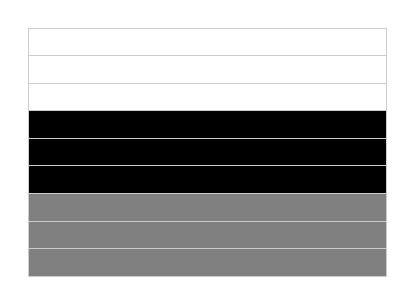
\begin{tikzpicture}[scale=0.35*\scalefactor]
\foreach \i in {0,...,2} {
  \draw[very thin,color=gray!40,fill=gray] (0, \i) rectangle (13, \i + 1);
}
\foreach \i in {3,...,5} {
  \draw[very thin,color=gray!40,fill=black] (0, \i) rectangle (13, \i + 1);
}
\foreach \i in {6,...,8} {
  \draw[very thin,color=gray!40,fill=white] (0, \i) rectangle (13, \i + 1);
}
\end{tikzpicture}
%
%epilight-skip-end
%epilight-replace dnf-c-color
}
\mycaption{Illustrating the Dutch national flag problem.\label{dnf-fig}}
\end{figure}



\p{dnf}%
Write a program that takes an \myindex{array}array $A$ and an index $i$ into $A$, and rearranges the elements such that all elements less than $A[i]$ (the ``pivot'') appear first, followed by elements equal to the pivot, followed by elements greater than the pivot.
%Your algorithm should have \myindex{$\mathcal{O}(1)$ space}$\mathcal{O}(1)$ space complexity and
%$\mathcal{O}(n)$ time complexity.




\autohint{LABELS_REMOVED}{Think about the partition step in quicksort.}

%dummy for rstrip
\ansbegin{dnf}
\label{solution-dnf}
The problem is trivial to solve with $\mathcal{O}(n)$ additional space, where $n$ is the length of $A$.
We form three lists, namely, elements less than the pivot, elements equal to the pivot, and elements greater than the pivot.
Consequently, we write these values into $A$.
The time complexity is $\mathcal{O}(n)$.

We can avoid using $\mathcal{O}(n)$ additional space at the cost of increased time complexity as follows.
%_TODO(THL): we can add "with extra run time" after "additional space" to give a heads up what is the algorithm here will be.
In the first stage, we iterate through $A$ starting from index $0$, then index $1$, etc.
In each iteration, we seek an element smaller than the pivot---as soon as we find it, we move it to the subarray of smaller elements via an exchange.
This moves all the elements less than the pivot to the start of the array. The second stage is similar to the first one, the difference being that we move elements greater than the pivot to the end of the array.
Code illustrating this approach is shown below.
%_TODO(AA): do you agree that we should show this?
%_TODO(AA): replace 0,1,2 with enum
\ifCpp
\begin{lstlisting}[language={[11]C++}]
typedef enum { RED, WHITE, BLUE } Color;

void DutchFlagPartition(int pivot_index, vector<Color>* A_ptr) {
  vector<Color>& A = *A_ptr;
  Color pivot = A[pivot_index];
  // First pass: group elements smaller than pivot.
  for (int i = 0; i < A.size(); ++i) {
    // Look for a smaller element.
    for (int j = i + 1; j < A.size(); ++j) {
      if (A[j] < pivot) {
        swap(A[i], A[j]);
        break;
      }
    }
  }
  // Second pass: group elements larger than pivot.
  for (int i = A.size() - 1; i >= 0 && A[i] >= pivot; --i) {
    // Look for a larger element. Stop when we reach an element less
    // than pivot, since first pass has moved them to the start of A.
    for (int j = i - 1; j >= 0 && A[j] >= pivot; --j) {
      if (A[j] > pivot) {
        swap(A[i], A[j]);
        break;
      }
    }
  }
}
\end{lstlisting}
\fi%ifCpp
\ifJava
\begin{lstlisting}[language=Java]
public static enum Color { RED, WHITE, BLUE }

public static void dutchFlagPartition(int pivotIndex, List<Color> A) {
  Color pivot = A.get(pivotIndex);
  // First pass: group elements smaller than pivot.
  for (int i = 0; i < A.size(); ++i) {
    // Look for a smaller element.
    for (int j = i + 1; j < A.size(); ++j) {
      if (A.get(j).ordinal() < pivot.ordinal()) {
        Collections.swap(A, i, j);
        break;
      }
    }
  }
  // Second pass: group elements larger than pivot.
  for (int i = A.size() - 1; i >= 0 && A.get(i).ordinal() >= pivot.ordinal();
       --i) {
    // Look for a larger element. Stop when we reach an element less
    // than pivot, since first pass has moved them to the start of A.
    for (int j = i - 1; j >= 0 && A.get(j).ordinal() >= pivot.ordinal();
         --j) {
      if (A.get(j).ordinal() > pivot.ordinal()) {
        Collections.swap(A, i, j);
        break;
      }
    }
  }
}
\end{lstlisting}
\fi%ifJava
\ifPython
\begin{lstlisting}[language=Python]
RED, WHITE, BLUE = range(3)


def dutch_flag_partition(pivot_index, A):
    pivot = A[pivot_index]
    # First pass: group elements smaller than pivot.
    for i in range(len(A)):
        # Look for a smaller element.
        for j in range(i + 1, len(A)):
            if A[j] < pivot:
                A[i], A[j] = A[j], A[i]
                break
    # Second pass: group elements larger than pivot.
    for i in reversed(range(len(A))):
        if A[i] < pivot:
            break
        # Look for a larger element. Stop when we reach an element less than
        # pivot, since first pass has moved them to the start of A.
        for j in reversed(range(i)):
            if A[j] > pivot:
                A[i], A[j] = A[j], A[i]
                break
\end{lstlisting}
\fi%ifPython

%_TODO(THL): improve description of two-pass solution based on Chris Zeng's email.
The additional space complexity is now $\mathcal{O}(1)$, but the time complexity is $\mathcal{O}(n^2)$, e.g., if $i = n/2$ and all elements before $i$ are greater than $A[i]$, and all elements after $i$ are less than $A[i]$.
%_TODO(THL): I am a little confused about the time complexity here as it seems 3 * O(n)?  The additional O(n) is due to the elements shifting in array?
%AA: it's because we keep scanning for the next element less than i, starting from 0, 1, 2, 3 etc.
%THL: I see the reason I confused, as your algorithm keeps scanning from the "begining" of the array, and the improved algorithm will scan from "last" location.  Do you want to emphysize that?
%AA: i have tried to emphasize this. it also makes me think that
% it's more natural to solve this in two passes--- first move elements less than key to beginning
% which is easy to do in O(n) using the trick of advancing from where you left off.
% second pass is identical to first with < replaced by ==.
% the single pass algo is less natural, more corner cases
%AA: can do in two passes but faster to do in one pass...
Intuitively, this approach has bad time complexity because in the first pass when searching for each additional element smaller than the pivot we start from the beginning.
However, there is no reason to start from so far back---we can begin from the last location we advanced to.
(Similar comments hold for the second pass.)
%To improve runtime, we should move elements to their correct locations immediately.

To improve time complexity, we make a single pass and move all the elements less than the pivot to the beginning.
In the second pass we move the larger elements to the end.
It is easy to perform each pass in a single iteration, moving out-of-place elements as soon as they are discovered.
%THL: code are added, and please use following \codefileinclude.
%AA: i've added a little more text. didnt see what you meant wrt the \codefileinclude, it's already present?
%THL: The above sentence of moving backward seems a little redundant.  Because moving larger one is the key we don't need to record where the smaller elements end.  Moving backwardly is just code optimization.
\ifCpp
\begin{lstlisting}[language={[11]C++}]
typedef enum { RED, WHITE, BLUE } Color;

void DutchFlagPartition(int pivot_index, vector<Color>* A_ptr) {
  vector<Color>& A = *A_ptr;
  Color pivot = A[pivot_index];
  // First pass: group elements smaller than pivot.
  int smaller = 0;
  for (int i = 0; i < A.size(); ++i) {
    if (A[i] < pivot) {
      swap(A[i], A[smaller++]);
    }
  }
  // Second pass: group elements larger than pivot.
  int larger = A.size() - 1;
  for (int i = A.size() - 1; i >= 0 && A[i] >= pivot; --i) {
    if (A[i] > pivot) {
      swap(A[i], A[larger--]);
    }
  }
}
\end{lstlisting}
\fi%ifCpp
\ifJava
\begin{lstlisting}[language=Java]
public static enum Color { RED, WHITE, BLUE }

public static void dutchFlagPartition(int pivotIndex, List<Color> A) {
  Color pivot = A.get(pivotIndex);
  // First pass: group elements smaller than pivot.
  int smaller = 0;
  for (int i = 0; i < A.size(); ++i) {
    if (A.get(i).ordinal() < pivot.ordinal()) {
      Collections.swap(A, smaller++, i);
    }
  }
  // Second pass: group elements larger than pivot.
  int larger = A.size() - 1;
  for (int i = A.size() - 1; i >= 0 && A.get(i).ordinal() >= pivot.ordinal();
       --i) {
    if (A.get(i).ordinal() > pivot.ordinal()) {
      Collections.swap(A, larger--, i);
    }
  }
}
\end{lstlisting}
\fi%ifJava
\ifPython
\begin{lstlisting}[language=Python]
RED, WHITE, BLUE = range(3)


def dutch_flag_partition(pivot_index, A):
    pivot = A[pivot_index]
    # First pass: group elements smaller than pivot.
    smaller = 0
    for i in range(len(A)):
        if A[i] < pivot:
            A[i], A[smaller] = A[smaller], A[i]
            smaller += 1
    # Second pass: group elements larger than pivot.
    larger = len(A) - 1
    for i in reversed(range(len(A))):
        if A[i] < pivot:
            break
        elif A[i] > pivot:
            A[i], A[larger] = A[larger], A[i]
            larger -= 1
\end{lstlisting}
\fi%ifPython
The time complexity is $\mathcal{O}(n)$ and the space complexity  is $\mathcal{O}(1)$.

The algorithm we now present is similar to the one sketched above.
The main difference is that it performs classification into elements less than, equal to, and greater than the pivot in a single pass.
This reduces runtime, at the cost of a trickier implementation.
%_TODO(THL): store the lists?  why list, I think it is more like the elements.
%AA: ok, i was thinking that the subarrays are like the lists, but have updated to elements to avoid confusion
We do this by maintaining four subarrays:
{\em bottom} (elements less than pivot), {\em middle} (elements equal to pivot), {\em unclassified}, and {\em top} (elements greater than pivot).
Initially, all elements are in {\em unclassified}.
%We use variables {\em smaller}, {\em equal}, and {\em larger} to
%track these groups.
%\begin{itemize}
%\item {\em bottom} is stored in \myindex{subarray}subarray $A[0,\mbox{\em smaller}-1]$.
%\item {\em middle} is stored in \myindex{subarray}subarray $A[\mbox{\em smaller},\mbox{\em equal}-1]$.
%\item {\em unclassified} is stored in \myindex{subarray}subarray $A[\mbox{\em equal},\mbox{\em larger}]$.
%\item {\em top} is stored in \myindex{subarray}subarray $A[\mbox{\em larger}+1,n-1]$.
%\end{itemize}
We iterate through elements in {\em unclassified}, and move elements into one of {\em bottom}, {\em middle}, and {\em top} groups according to the relative order between the incoming unclassified element and the pivot.

As a concrete example, suppose the array is currently $A = \langle -3, 0, -1, 1, 1, ?, ?, ?, 4, 2\rangle$, where the pivot is $1$ and $?$ denotes unclassified elements. There are three possibilities for the first unclassified element, $A[5]$.
\begin{itemize}
\item $A[5]$ is less than the pivot, e.g., $A[5] = -5$.
We exchange it with the first $1$, i.e., the new array is $\langle -3, 0, -1, -5, 1, 1, ?, ?, 4, 2\rangle$.
\item $A[5]$ is equal to the pivot, i.e., $A[5] = 1$.
We do not need to move it, we just advance to the next unclassified element, i.e., the array is $\langle -3, 0, -1, 1, 1, 1, ?, ?, 4, 2\rangle$.
\item $A[5]$ is greater than the pivot, e.g., $A[5] = 3$.
We exchange it with the last unclassified element, i.e., the new array is $\langle -3, 0, -1, 1, 1, ?, ?, 3, 4, 2\rangle$.
\end{itemize}
Note how the number of unclassified elements reduces by one in each case.
\ifCpp
\begin{lstlisting}[language={[11]C++}]
typedef enum { RED, WHITE, BLUE } Color;

void DutchFlagPartition(int pivot_index, vector<Color>* A_ptr) {
  vector<Color>& A = *A_ptr;
  Color pivot = A[pivot_index];
  /**
   * Keep the following invariants during partitioning:
   * bottom group: A[0, smaller - 1].
   * middle group: A[smaller, equal - 1].
   * unclassified group: A[equal, larger - 1].
   * top group: A[larger, A.size() - 1].
   */
  int smaller = 0, equal = 0, larger = A.size();
  // Keep iterating as long as there is an unclassified element.
  while (equal < larger) {
    // A[equal] is the incoming unclassified element.
    if (A[equal] < pivot) {
      swap(A[smaller++], A[equal++]);
    } else if (A[equal] == pivot) {
      ++equal;
    } else {  // A[equal] > pivot.
      swap(A[equal], A[--larger]);
    }
  }
}
\end{lstlisting}
\fi%ifCpp
\ifJava
\begin{lstlisting}[language=Java]
public static enum Color { RED, WHITE, BLUE }

public static void dutchFlagPartition(int pivotIndex, List<Color> A) {
  Color pivot = A.get(pivotIndex);
  /**
   * Keep the following invariants during partitioning:
   * bottom group: A.subList(0, smaller).
   * middle group: A.subList(smaller, equal).
   * unclassified group: A.subList(equal, larger).
   * top group: A.subList(larger, A.size()).
   */
  int smaller = 0, equal = 0, larger = A.size();
  // Keep iterating as long as there is an unclassified element.
  while (equal < larger) {
    // A.get(equal) is the incoming unclassified element.
    if (A.get(equal).ordinal() < pivot.ordinal()) {
      Collections.swap(A, smaller++, equal++);
    } else if (A.get(equal).ordinal() == pivot.ordinal()) {
      ++equal;
    } else { // A.get(equal) > pivot.
      Collections.swap(A, equal, --larger);
    }
  }
}
\end{lstlisting}
\fi%ifJava
\ifPython
\begin{lstlisting}[language=Python]
RED, WHITE, BLUE = range(3)


def dutch_flag_partition(pivot_index, A):
    pivot = A[pivot_index]
    # Keep the following invariants during partitioning:
    # bottom group: A[:smaller].
    # middle group: A[smaller:equal].
    # unclassified group: A[equal:larger].
    # top group: A[larger:].
    smaller, equal, larger = 0, 0, len(A)
    # Keep iterating as long as there is an unclassified element.,
    while equal < larger:
        # A[equal] is the incoming unclassified element.
        if A[equal] < pivot:
            A[smaller], A[equal] = A[equal], A[smaller]
            smaller, equal = smaller + 1, equal + 1
        elif A[equal] == pivot:
            equal += 1
        else:  # A[equal] > pivot.
            larger -= 1
            A[equal], A[larger] = A[larger], A[equal]
\end{lstlisting}
\fi%ifPython
Each iteration decreases the size of {\em unclassified} by $1$, and the time spent within each iteration is $\mathcal{O}(1)$, implying the time complexity is $\mathcal{O}(n)$.
The space complexity is clearly $\mathcal{O}(1)$.
%TODO(THL,2.0): We are still explaining the code..
% use this figure: http://www.csse.monash.edu.au/~lloyd/tildeAlgDS/Sort/Flag/

%_TODO(AA): how much of this is relevant? eg do we need BST reference?
% When an array consists of entries from a small set of keys, e.g., $\{0,1,2\}$, one
% way to sort it is to count the number of occurrences of each key. Consequently,
% enumerate the keys in sorted order and write the corresponding number of keys
% to the array. If a \myindex{BST}BST is used for counting, the time complexity
% of this approach is $\mathcal{O}(n\log k)$, where $n$ is the array length
% and $k$ is the number of keys.
% This is known as \myindex{sorting!counting sort}\myindex{counting sort|textbf}counting sort.
%
% \myindex{sorting!counting sort}\myindex{counting sort}Counting sort, as
% just described, does not differentiate among different
% objects with the same key value.
% The current problem is concerned with a special case of \myindex{sorting!counting sort}\myindex{counting sort}counting sort
% when entries are objects rather than keys.
% %epilight-skip-begin
% Problem~\vref{counting-sort} addresses the general problem.
% %epilight-skip-end
% %Problems~\vref{dnf} and~\vref{counting-sort} are concerned with
% %implementing counting sort for arrays holding general
% %objects using \myindex{$\mathcal{O}(1)$ space}$\mathcal{O}(1)$ additional space.
% %To make \myindex{sorting!counting sort}\myindex{counting sort}counting sort work when the array
% %entries are objects and the keys are a specific field, it is necessary to
% %have another array to write the original entries to.
% %Consequently, the sort does not run in \myindex{$\mathcal{O}(1)$ space}$\mathcal{O}(1)$ space.
% %In contrast, the Dutch national flag partitioning problem calls for an algorithm
% %that runs in \myindex{$\mathcal{O}(1)$ space}$\mathcal{O}(1)$ space.

%following renewcommand is for the referencing two figures, the original default one is "\ref{#1} to~\ref{#2}
\renewcommand{\reftextlabelrange}[2]{\ref{#1} and~\ref{#2}}%

\variant{Assuming that keys take one of three values, reorder the array so that all objects with the same key appear together.
The order of the \myindex{subarray}subarrays is not important.
For example, both Figures \myvrefrange{dnf-fig-b}{dnf-fig-c}are valid answers for Figure~\vref{dnf-fig-a}.
Use \myindex{$\mathcal{O}(1)$ space}$\mathcal{O}(1)$ additional space and $\mathcal{O}(n)$ time.}

\variant{Given an array $A$ of $n$ objects with keys that takes one of four values,
reorder the array so that all objects that have the same key appear together.
Use \myindex{$\mathcal{O}(1)$ space}$\mathcal{O}(1)$ additional space and $\mathcal{O}(n)$ time.}

\variant{Given an array $A$ of $n$ objects with Boolean-valued keys,
reorder the array so that objects that have the key false appear first.
Use \myindex{$\mathcal{O}(1)$ space}$\mathcal{O}(1)$ additional space and $\mathcal{O}(n)$ time.}

\variant{Given an array $A$ of $n$ objects with Boolean-valued keys,
reorder the array so that objects that have the key false appear first.
The relative ordering of objects with key true should not change.
Use \myindex{$\mathcal{O}(1)$ space}$\mathcal{O}(1)$ additional space and $\mathcal{O}(n)$ time.}

\ansend

% %coffin
% %TODO(AA): remove
% \skullindexsection{Lazy initialization}
% \label{lazy-init}
% You have some code which allocates a Boolean-valued \myindex{array}array $A$.
% The memory manager allocates this \myindex{array}array in $\mathcal{O}(1)$ time,
% but the contents of the allocated \myindex{array}array are arbitrary. You
% would like to initialize all the entries to $0$.
% The length $n$ of $A$ is potentially huge and
% you want to avoid the $\mathcal{O}(n)$ time complexity of initialization.
%
% One way to check if an \myindex{array}array entry has been written to is to store the indices
% that have been written to in a \myindex{hash table}hash table. Suppose the drawbacks of a \myindex{hash table}hash table---poor performance
% if the \myindex{hash code}hash codes are not spread out, and
% the need for \myindex{rehashing}rehashing---are not acceptable.
%


% \p{lazy-init}%
% Design a deterministic scheme by which reads and writes
% to an uninitialized \myindex{array}array can be made in $\mathcal{O}(1)$ time. You may
% use $\mathcal{O}(n)$ additional storage; reads to uninitialized
% entry should return false.
%
% \hint{First use another array to track the initialization status of each entry of $A$.
% Improve on this solution if you know the number of writes to uninitialized entries.}
%
% \ansbegin{lazy-init}
% Create an (uninitialized) \myindex{array}array $P$ of $n$ pointers.
% The \myindex{array}array $P$ will maintain a pointer for each initialized entry
% of $A$ to a back pointer on another array~$S$,
% itself an (uninitialized) array of $n$ integers. An integer-valued
% variable $t$ indicates the first empty entry in $S$; initially, $t = 0$.
%
% Each time entry $i$ from $A$ is to be read,
% we can check if that entry has been written to before by examining $P[i]$.
% If $P[i]$ is outside $[0,t-1]$, $A[i]$ is uninitialized.
% However, even if $P[i]$ is uninitialized, it may lie in $[0,t-1]$.
% We look at the ``back pointer'' stored in $S[P[i]]$ and confirm that it is indeed $i$.
% Critically, we know if $S[P[i]]$ is initialized by checking $0 \leq P[i] < t-1$.
%
% The first time entry $i$ is written in $A$, we set $S[t]$ to $i$,
% $P[i]$ to $t$ and increment $t$. (We can check
% that the write is the first write to $A[i]$ by first performing a read
% and checking if the entry is uninitialized.)
%
% The approach is illustrated in Figure~\vref{lazy-init-fig}.
% The first three entries written are at indices $7$, $2$, and $1$,
% in that order. Checking if the entry at index $6$ is initialized entails
% examining $P[6]$. If the value in $P[6]$ is not in $[0,2]$,
% $A[6]$ is uninitialized. If it is a valid index, e.g., $1$,
% we check if $S[1]$ is $6$. For this example,
% $P[6] = 1 \mbox{ and } S[P[6]] = 2 \neq 6$, so $A[6]$ is uninitialized.
%
% \begin{figure}[htb]
% \centering
% \input{graphics/uninit_array}
% \mycaption{ \label{lazy-init-fig} Initializing an array in $\mathcal{O}(1)$ time.}
% \end{figure}
%
% \codefileinclude{lazy-init.cc}
%
% \ansend

%_TODO(THL): check example
%\indexsection{Compute the max difference}
%epilight-skip-begin
\ds{Multidimensional arrays}

Thus far we have focused our attention in this chapter on one-dimensional arrays.  We now
turn our attention to multidimensional arrays.
A $2$D~array in an array whose
entries are themselves arrays; the concept generalizes naturally to $k$ dimensional arrays.

Multidimensional
arrays arise in image processing, board games, graphs,
modeling spatial phenomenon, etc. Often, but not always,
the arrays that constitute the entries of a $2$D~array $A$ have the same length, in which
case we refer to $A$ as being an $m \times n$ rectangular array (or sometimes just
an $m \times n$ array), where $m$ is the number
of entries in $A$, and $n$ the number of entries in $A[0]$.
The elements within a $2$D~array $A$ are often referred to by their {\em row} and {\em column}
indices $i$ and $j$, and written as $A[i][j]$.
%epilight-skip-end

\indexsection{The Sudoku checker problem}
\label{sudoku-checker}
\myindex{Sudoku|textbf}Sudoku is a popular logic-based combinatorial number placement puzzle.
The objective is to fill a $9\times 9$ grid with digits subject to the constraint that each column,
each row, and each of the nine $3 \times 3$ sub-grids that compose the grid
contains unique integers in $[1,9]$. The grid is initialized with a partial
assignment as shown in Figure~\vref{sudoku-checker-fig-a};
a complete solution is shown in Figure~\vref{sudoku-checker-fig-b}.

\begin{figure}[htb]
\doscalesixnine
\centering
\mysubbottom{Partial assignment.}{sudoku-checker-fig-a}{graphics/sudoku}
\hspace{10pt} % increase the space between subfigures
\mysubbottom{A complete solution.}{sudoku-checker-fig-b}{graphics/sudoku-solved}
\mycaption{\myindex{Sudoku}Sudoku configurations.\label{sudoku-checker-fig}}
\end{figure}



\p{sudoku-checker}%
Check whether a $9 \times 9$ \myindex{$2$D array}$2$D array representing a partially
completed \myindex{Sudoku}Sudoku is valid. Specifically, check that
no row, column, or $3\times3$ \myindex{$2$D subarray}$2$D subarray contains duplicates.
A $0$-value in the \myindex{$2$D array}$2$D array indicates that entry is blank; every
other entry is in $[1,9]$.
\s{bbs forum}




\autohint{LABELS_REMOVED}{Directly test the constraints.  Use an array to encode sets.}

%dummy for rstrip
\ansbegin{sudoku-checker}
\label{solution-sudoku-checker}
There is no real scope for algorithm optimization in this problem---it's all about writing clean code.

We need to check nine \myindex{row constraint}\myindex{constraint!row}row constraints, nine \myindex{column constraint}\myindex{constraint!column}column constraints, and nine \myindex{sub-grid constraint}\myindex{constraint!sub-grid}sub-grid constraints.
It is convenient to use \myindex{bit array}bit arrays to test for constraint violations, that is to ensure no
number in $[1,9]$ appears more than once.
%_TODO(AA,THL): reference effective C++ book for use of deque<bool> instead of vetor<bool>q. same for
%pointer and reference (why arguments are sent, because we dont want to have reader look at signature)
%_TODO(THL): Need test for this file.
\ifCpp
\begin{lstlisting}[language={[11]C++}]
// Check if a partially filled matrix has any conflicts.
bool IsValidSudoku(const vector<vector<int>>& partial_assignment) {
  // Check row constraints.
  for (int i = 0; i < partial_assignment.size(); ++i) {
    if (HasDuplicate(partial_assignment, i, i + 1, 0,
                     partial_assignment.size())) {
      return false;
    }
  }

  // Check column constraints.
  for (int j = 0; j < partial_assignment.size(); ++j) {
    if (HasDuplicate(partial_assignment, 0, partial_assignment.size(), j,
                     j + 1)) {
      return false;
    }
  }

  // Check region constraints.
  int region_size = sqrt(partial_assignment.size());
  for (int I = 0; I < region_size; ++I) {
    for (int J = 0; J < region_size; ++J) {
      if (HasDuplicate(partial_assignment, region_size * I,
                       region_size * (I + 1), region_size * J,
                       region_size * (J + 1))) {
        return false;
      }
    }
  }
  return true;
}

// Return true if subarray partial_assignment[start_row, end_row -
// 1][start_col, end_col - 1] contains any duplicates in {1, 2, ...,
// partial_assignment.size()}; otherwise return false.
bool HasDuplicate(const vector<vector<int>>& partial_assignment,
                  int start_row, int end_row, int start_col, int end_col) {
  deque<bool> is_present(partial_assignment.size() + 1, false);
  for (int i = start_row; i < end_row; ++i) {
    for (int j = start_col; j < end_col; ++j) {
      if (partial_assignment[i][j] != 0 &&
          is_present[partial_assignment[i][j]]) {
        return true;
      }
      is_present[partial_assignment[i][j]] = true;
    }
  }
  return false;
}
\end{lstlisting}
\fi%ifCpp
\ifJava
\begin{lstlisting}[language=Java]
// Check if a partially filled matrix has any conflicts.
public static boolean isValidSudoku(List<List<Integer>> partialAssignment) {
  // Check row constraints.
  for (int i = 0; i < partialAssignment.size(); ++i) {
    if (hasDuplicate(partialAssignment, i, i + 1, 0,
                     partialAssignment.size())) {
      return false;
    }
  }

  // Check column constraints.
  for (int j = 0; j < partialAssignment.size(); ++j) {
    if (hasDuplicate(partialAssignment, 0, partialAssignment.size(), j,
                     j + 1)) {
      return false;
    }
  }

  // Check region constraints.
  int regionSize = (int)Math.sqrt(partialAssignment.size());
  for (int I = 0; I < regionSize; ++I) {
    for (int J = 0; J < regionSize; ++J) {
      if (hasDuplicate(partialAssignment, regionSize * I,
                       regionSize * (I + 1), regionSize * J,
                       regionSize * (J + 1))) {
        return false;
      }
    }
  }
  return true;
}

// Return true if subarray
// partialAssignment[startRow, endRow][startCol, endCol] contains any
// duplicates in {1, 2, ..., partialAssignment.size()}; otherwise return
// false.
private static boolean hasDuplicate(List<List<Integer>> partialAssignment,
                                    int startRow, int endRow, int startCol,
                                    int endCol) {
  List<Boolean> isPresent = new ArrayList<>(
      Collections.nCopies(partialAssignment.size() + 1, false));
  for (int i = startRow; i < endRow; ++i) {
    for (int j = startCol; j < endCol; ++j) {
      if (partialAssignment.get(i).get(j) != 0
          && isPresent.get(partialAssignment.get(i).get(j))) {
        return true;
      }
      isPresent.set(partialAssignment.get(i).get(j), true);
    }
  }
  return false;
}
\end{lstlisting}
\fi%ifJava
\ifPython
\begin{lstlisting}[language=Python]
# Check if a partially filled matrix has any conflicts.
def is_valid_sudoku(partial_assignment):
    # Return True if subarray
    # partial_assignment[start_row:end_row][start_col:end_col] contains any
    # duplicates in {1, 2, ..., len(partial_assignment)}; otherwise return
    # False.
    def has_duplicate(block):
        block = list(filter(lambda x: x != 0, block))
        return len(block) != len(set(block))

    n = len(partial_assignment)
    # Check row and column constraints.
    if any(
            has_duplicate([partial_assignment[i][j] for j in range(n)]) or
            has_duplicate([partial_assignment[j][i] for j in range(n)])
            for i in range(n)):
        return False

    # Check region constraints.
    region_size = int(math.sqrt(n))
    return all(not has_duplicate([
        partial_assignment[a][b]
        for a in range(region_size * I, region_size * (I + 1))
        for b in range(region_size * J, region_size * (J + 1))
    ]) for I in range(region_size) for J in range(region_size))


# Pythonic solution that exploits the power of list comprehension.
def is_valid_sudoku_pythonic(partial_assignment):
    region_size = int(math.sqrt(len(partial_assignment)))
    return max(collections.Counter(
        k for i, row in enumerate(partial_assignment) for j, c in enumerate(row)
        if c != 0
        for k in ((i, str(c)), (str(c), j
                                ), (i / region_size, j / region_size, str(c))))
               .values(),
               default=0) <= 1


\end{lstlisting}
\fi%ifPython
The time complexity of this algorithm for an $n \times n$ Sudoku grid with
$\sqrt n \times \sqrt n$ subgrids is $\mathcal{O}(n^2) + \mathcal{O}(n^2) + \mathcal{O}(n^2/(\sqrt n)^2 \times (\sqrt n)^2)
= \mathcal{O}(n^2)$; the terms correspond to the complexity to check
$n$ \myindex{row constraint}\myindex{constraint!row}row constraints, the $n$ \myindex{column constraint}\myindex{constraint!column}column constraints, and the $n$ subgrid constraints, respectively.
The memory usage is dominated by the \myindex{bit array}bit array used
to check the constraints, so the  space complexity is $\mathcal{O}(n)$.

Solution~\vref{solution-sudoku-solver} describes how to solve \myindex{Sudoku}Sudoku instances.

\ansend

\indexsection{Compute the spiral ordering of a $2$D array}
\label{spiral-matrix}
%_TODO(AA): use C0, R1, etc. to label and columns
A \myindex{$2$D array}$2$D array can be written as a sequence
in several orders---the most natural ones being row-by-row or column-by-column.
In this problem we explore the problem of writing the \myindex{$2$D array}$2$D array in spiral order.
For example, the spiral ordering for the \myindex{$2$D array}$2$D array in
%_TODO(THL): I think we should use < > with comma separated value for the following example.
Figure~\vref{spiral-matrix-fig-a} is
$\langle 1, 2, 3, 6, 9, 8, 7, 4, 5\rangle$.
For Figure~\vref{spiral-matrix-fig-b}, the spiral ordering is
$\langle 1, 2, 3,  4,  8,  12,  16,  15,  14,  13,  9,  5,  6,  7,  11,  10\rangle$.

\begin{figure}[htb]
\doscalesixnine
\centering
\subbottom[\textsf{Spiral ordering for a $3 \times 3$ array.}]{\label{spiral-matrix-fig-a}%
%epilight-skip-begin
\tikzstyle{edge} = [draw,line width=0.3pt,arrows={-latex'},black!100]
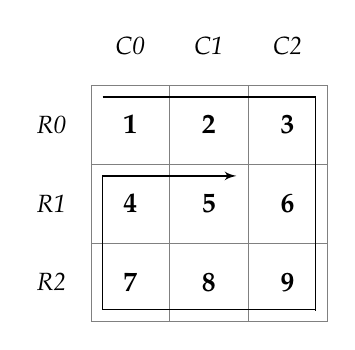
\begin{tikzpicture}[scale=1.0*\scalefactor,auto,swap]
\newcommand{\segmentrightdown}[4]{
  \draw[edge] (#1+0.85,#2-0.15) -- (#3+0.85,#4-0.15);
  \draw[fill] (#1+0.85,#2-0-0.15) circle (0.05);
}

\newcommand{\lineshift}{0.011}
\draw[help lines,step=1] (0,0) grid (3,3);

\draw[line width=0.5pt, arrows={-},black!100] (0.15,2.85) -- (2.85+\lineshift,2.85);
\draw[line width=0.5pt, arrows={-},black!100] (2.85,2.85) -- (2.85,0.15-\lineshift);
\draw[line width=0.5pt, arrows={-},black!100] (2.85,0.15) -- (0.15-\lineshift,0.15);
\draw[line width=0.5pt, arrows={-},black!100] (0.15,0.15) -- (0.15,1.85+\lineshift);
\draw[line width=0.5pt, arrows={-latex'},black!100] (0.15,1.85) -- (1.85,1.85);
\node at (0.5,2.5) {\textbf{1}};
\node at (1.5,2.5) {\textbf{2}};
\node at (2.5,2.5) {\textbf{3}};
\node at (0.5,1.5) {\textbf{4}};
\node at (1.5,1.5) {\textbf{5}};
\node at (2.5,1.5) {\textbf{6}};
\node at (0.5,0.5) {\textbf{7}};
\node at (1.5,0.5) {\textbf{8}};
\node at (2.5,0.5) {\textbf{9}};

\node at (0.5,3.5) {\emph{\small C0}};
\node at (1.5,3.5) {\emph{\small C1}};
\node at (2.5,3.5) {\emph{\small C2}};

\node at (-0.5,2.5) {\emph{\small R0}};
\node at (-0.5,1.5) {\emph{\small R1}};
\node at (-0.5,0.5) {\emph{\small R2}};


\end{tikzpicture}
%
%epilight-skip-end
%epilight-replace dnf-a-color
}
\hspace{16pt} % incrase the space betweeen subfigures
\subbottom[\textsf{Spiral ordering for a $4 \times 4$ array.}]{\label{spiral-matrix-fig-b}%
%epilight-skip-begin
\tikzstyle{edge} = [draw,line width=0.3pt,arrows={-latex'},black!100]
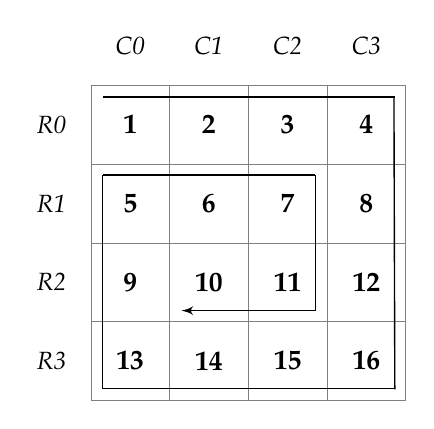
\begin{tikzpicture}[scale=1.0*\scalefactor,auto,swap]
\newcommand{\segmentrightdown}[4]{
  \draw[edge] (#1+0.85,#2-0.15) -- (#3+0.85,#4-0.15);
  \draw[fill] (#1+0.85,#2-0-0.15) circle (0.05);
}

\newcommand{\lineshift}{0.011}
\draw[help lines,step=1] (0,0) grid (4,4);

\draw[line width=0.5pt, arrows={-},black!100] (0.15,3.85) -- (3.85+\lineshift,3.85);
\draw[line width=0.5pt, arrows={-},black!100] (3.85,3.85) -- (3.85+\lineshift,0.15-\lineshift);
\draw[line width=0.5pt, arrows={-},black!100] (3.85,0.15) -- (0.15-\lineshift,0.15);
\draw[line width=0.5pt, arrows={-},black!100] (0.15,0.15) -- (0.15,2.85+\lineshift);

\draw[line width=0.5pt, arrows={-},black!100] (0.15,2.85+\lineshift) -- (2.85,2.85+\lineshift);
\draw[line width=0.5pt, arrows={-},black!100] (2.85,2.85+\lineshift) -- (2.85,1.15-\lineshift);

\draw[line width=0.5pt, arrows={-latex'},black!100] (2.85,1.15-\lineshift) -- (1.15,1.15-\lineshift);

\node at (0.5,3.5) {\textbf{1}};
\node at (1.5,3.5) {\textbf{2}};
\node at (2.5,3.5) {\textbf{3}};
\node at (3.5,3.5) {\textbf{4}};

\node at (0.5,2.5) {\textbf{5}};
\node at (1.5,2.5) {\textbf{6}};
\node at (2.5,2.5) {\textbf{7}};
\node at (3.5,2.5) {\textbf{8}};

\node at (0.5,1.5) {\textbf{9}};
\node at (1.5,1.5) {\textbf{10}};
\node at (2.5,1.5) {\textbf{11}};
\node at (3.5,1.5) {\textbf{12}};

\node at (0.5,0.5) {\textbf{13}};
\node at (1.5,0.5) {\textbf{14}};
\node at (2.5,0.5) {\textbf{15}};
\node at (3.5,0.5) {\textbf{16}};

\node at (0.5,4.5) {\emph{\small C0}};
\node at (1.5,4.5) {\emph{\small C1}};
\node at (2.5,4.5) {\emph{\small C2}};
\node at (3.5,4.5) {\emph{\small C3}};

\node at (-0.5,3.5) {\emph{\small R0}};
\node at (-0.5,2.5) {\emph{\small R1}};
\node at (-0.5,1.5) {\emph{\small R2}};
\node at (-0.5,0.5) {\emph{\small R3}};


\end{tikzpicture}
%
%epilight-skip-end
%epilight-replace dnf-b-color
}
\mycaption{Spiral orderings. Column and row ids are specified above
and to the left of the matrix, i.e., $1$ is at entry $(0,0)$. \label{spiral-matrix-fig}}
\end{figure}



\p{spiral-matrix}%
Write a program which takes an $n \times n$ \myindex{$2$D array}$2$D array and returns the spiral
ordering of the array.
%_TODO(THL): I will say remove the following sentence and use n * n in the above setence.  Besides, I would like to remove the n * n in the introduction part probably.




\autohint{LABELS_REMOVED}{Use \myindex{case analysis}case analysis and divide-and-conquer.}

%dummy for rstrip
\ansbegin{spiral-matrix}
\label{solution-spiral-matrix}
It is natural to solve this problem starting from the outside, and working to the center.
The naive approach begins by adding the first row, which consists of $n$ elements. Next we add the
$n-1$ remaining elements of the last column, then the $n-1$ remaining elements of the last row,
and then the $n-2$ remaining elements of the first column.
The lack of uniformity makes it hard to get the code right.

Here is a uniform way of adding the boundary. Add the first $n-1$ elements of the first row.
Then add the first $n-1$ elements of the last column. Then add the last $n-1$ elements of the last row
in reverse order. Finally, add the last $n-1$ elements of the first column in reverse order.
%The outermost elements of an $n \times n$ \myindex{$2$D array}$2$D array can be written in spiral order using four iterations: elements $(0,0)$ to
%(0,n-2)$, then elements $(0,n-1)$ to $(n-2,n-1)$, followed by elements $(n-1,n-1)$ to $(n-1,1)$, and finally
%lements $(n-1,0)$ to $(1,0)$.

After this, we are left with the problem of adding the elements of an
$(n-2) \times (n-2)$ \myindex{$2$D array}$2$D array in spiral order.
This leads to an iterative algorithm that adds
the outermost elements of $n\times n, (n-2) \times (n - 2),(n-4)\times (n-4),\dots$ \myindex{$2$D array}$2$D arrays.
Note that a matrix of odd dimension has a corner-case, namely when we reach its center.
%This algorithm is implemented below in Java:
% the variable \texttt{offset} is used to
%AA: done


As an example, for the $3 \times 3$ array in Figure~\vref{spiral-matrix-fig-a},
%_TODO(THL): first 2 or first two?  Similarly for the paragraph below, first three?
we would add $1,2$ (first two elements of the first row), then
$3,6$ (first two elements of the last column), then
$9,8$ (last two elements of the last row), then
$7,4$ (last two elements of the first column). We are now left
with the $1 \times 1$ array, whose sole element is $5$. After processing it, all elements are processed.

For the $4\times 4$ array  in Figure~\vref{spiral-matrix-fig-b},
we would add $1,2,3$ (first three elements of the first row), then
$4,8,12$ (first three elements of the last column), then
$16,15,14$ (last three elements of the last row), then
$13,9,5$ (last three elements of the first column). We are now left
with a $2 \times 2$ matrix, which we process similarly in the order $6,7,11,10$, after which
all elements are processed.
\ifCpp
\begin{lstlisting}[language={[11]C++}]
vector<int> MatrixInSpiralOrder(const vector<vector<int>>& square_matrix) {
  vector<int> spiral_ordering;
  for (int offset = 0; offset < ceil(0.5 * square_matrix.size()); ++offset) {
    MatrixLayerInClockwise(square_matrix, offset, &spiral_ordering);
  }
  return spiral_ordering;
}

void MatrixLayerInClockwise(const vector<vector<int>>& square_matrix,
                            int offset, vector<int>* spiral_ordering) {
  if (offset == square_matrix.size() - offset - 1) {
    // square_matrix has odd dimension, and we are at the center of
    // square_matrix.
    spiral_ordering->emplace_back(square_matrix[offset][offset]);
    return;
  }

  for (int j = offset; j < square_matrix.size() - offset - 1; ++j) {
    spiral_ordering->emplace_back(square_matrix[offset][j]);
  }
  for (int i = offset; i < square_matrix.size() - offset - 1; ++i) {
    spiral_ordering->emplace_back(
        square_matrix[i][square_matrix.size() - offset - 1]);
  }
  for (int j = square_matrix.size() - offset - 1; j > offset; --j) {
    spiral_ordering->emplace_back(
        square_matrix[square_matrix.size() - offset - 1][j]);
  }
  for (int i = square_matrix.size() - offset - 1; i > offset; --i) {
    spiral_ordering->emplace_back(square_matrix[i][offset]);
  }
}
\end{lstlisting}
\fi%ifCpp
\ifJava
\begin{lstlisting}[language=Java]
public static List<Integer> matrixInSpiralOrder(
    List<List<Integer>> squareMatrix) {
  List<Integer> spiralOrdering = new ArrayList<>();
  for (int offset = 0; offset < Math.ceil(0.5 * squareMatrix.size());
       ++offset) {
    matrixLayerInClockwise(squareMatrix, offset, spiralOrdering);
  }
  return spiralOrdering;
}

private static void matrixLayerInClockwise(List<List<Integer>> squareMatrix,
                                           int offset,
                                           List<Integer> spiralOrdering) {
  if (offset == squareMatrix.size() - offset - 1) {
    // squareMatrix has odd dimension, and we are at its center.
    spiralOrdering.add(squareMatrix.get(offset).get(offset));
    return;
  }

  for (int j = offset; j < squareMatrix.size() - offset - 1; ++j) {
    spiralOrdering.add(squareMatrix.get(offset).get(j));
  }
  for (int i = offset; i < squareMatrix.size() - offset - 1; ++i) {
    spiralOrdering.add(
        squareMatrix.get(i).get(squareMatrix.size() - offset - 1));
  }
  for (int j = squareMatrix.size() - offset - 1; j > offset; --j) {
    spiralOrdering.add(
        squareMatrix.get(squareMatrix.size() - offset - 1).get(j));
  }
  for (int i = squareMatrix.size() - offset - 1; i > offset; --i) {
    spiralOrdering.add(squareMatrix.get(i).get(offset));
  }
}
\end{lstlisting}
\fi%ifJava
\ifPython
\begin{lstlisting}[language=Python]
def matrix_in_spiral_order(square_matrix):
    def matrix_layer_in_clockwise(offset):
        if offset == len(square_matrix) - offset - 1:
            # square_matrix has odd dimension, and we are at the center of the
            # matrix square_matrix.
            spiral_ordering.append(square_matrix[offset][offset])
            return

        spiral_ordering.extend(square_matrix[offset][offset:-1 - offset])
        spiral_ordering.extend(
            list(zip(*square_matrix))[-1 - offset][offset:-1 - offset])
        spiral_ordering.extend(
            square_matrix[-1 - offset][-1 - offset:offset:-1])
        spiral_ordering.extend(
            list(zip(*square_matrix))[offset][-1 - offset:offset:-1])

    spiral_ordering = []
    for offset in range((len(square_matrix) + 1) // 2):
        matrix_layer_in_clockwise(offset)
    return spiral_ordering
\end{lstlisting}
\fi%ifPython

\ifPython
The time complexity is $\mathcal{O}(n^2)$.
\else
The time complexity is $\mathcal{O}(n^2)$ and the space complexity is \myindex{$\mathcal{O}(1)$ space}$\mathcal{O}(1)$.
\fi

%An alternate solution writes $0$ into \myindex{array}array entries to indicate they have been processed,
%_TODO(AA, texttt): following needs some works
%AA: please check my wording
%THL: your text looks like explaining code implementation.  We can try to use some other way to explain this.
The above solution uses four iterations which are almost identical.
Now we present a solution that uses a single
iteration that tracks the next element to process
and the direction---left,right,up,down---to advance in.
Think of the matrix as laid out on a $2D$ grid with
$X$- and $Y$-axes.  The pair $(i,j)$ denotes the entry in Column~$i$ and Row~$j$.
Let $(x,y)$ be the next element to process.
Initially we move to the right (incrementing $x$ until $(n-1,0)$ is processed).
Then we move down (incrementing $y$ until $(n-1,n-1)$ is processed).
Then we move left (decrementing $x$ until $(0,n-1)$ is processed).
Then we move up (decrementing $y$ until $(0,1)$ is processed).
Note that we stop at $1$, not $0$, since $(0,0)$ was already processed.
We record that an element has already been processed by setting it to $0$, which is
assumed to be a value that is not already present in the array. (Any value not in the
array works too.)
After processing $(0,1)$ we move to the right till we get to $(n-2,1)$ (since $(n-2,0)$ was
already processed). This method is applied until all elements are processed.
\ifCpp
\begin{lstlisting}[language={[11]C++}]
vector<int> MatrixInSpiralOrder(vector<vector<int>> square_matrix) {
  const array<array<int, 2>, 4> kShift = {{{0, 1}, {1, 0}, {0, -1}, {-1, 0}}};
  int dir = 0, x = 0, y = 0;
  vector<int> spiral_ordering;

  for (int i = 0; i < square_matrix.size() * square_matrix.size(); ++i) {
    spiral_ordering.emplace_back(square_matrix[x][y]);
    square_matrix[x][y] = 0;
    int next_x = x + kShift[dir][0], next_y = y + kShift[dir][1];
    if (next_x < 0 || next_x >= square_matrix.size() || next_y < 0 ||
        next_y >= square_matrix.size() ||
        square_matrix[next_x][next_y] == 0) {
      dir = (dir + 1) % 4;
      next_x = x + kShift[dir][0], next_y = y + kShift[dir][1];
    }
    x = next_x, y = next_y;
  }
  return spiral_ordering;
}
\end{lstlisting}
\fi%ifCpp
\ifJava
\begin{lstlisting}[language=Java]
public static List<Integer> matrixInSpiralOrder(
    List<List<Integer>> squareMatrix) {
  final int[][] SHIFT = {{0, 1}, {1, 0}, {0, -1}, {-1, 0}};
  int dir = 0, x = 0, y = 0;
  List<Integer> spiralOrdering = new ArrayList<>();

  for (int i = 0; i < squareMatrix.size() * squareMatrix.size(); ++i) {
    spiralOrdering.add(squareMatrix.get(x).get(y));
    squareMatrix.get(x).set(y, 0);
    int nextX = x + SHIFT[dir][0], nextY = y + SHIFT[dir][1];
    if (nextX < 0 || nextX >= squareMatrix.size() || nextY < 0
        || nextY >= squareMatrix.size()
        || squareMatrix.get(nextX).get(nextY) == 0) {
      dir = (dir + 1) % 4;
      nextX = x + SHIFT[dir][0];
      nextY = y + SHIFT[dir][1];
    }
    x = nextX;
    y = nextY;
  }
  return spiralOrdering;
}
\end{lstlisting}
\fi%ifJava
\ifPython
\begin{lstlisting}[language=Python]
def matrix_in_spiral_order(square_matrix):
    SHIFT = ((0, 1), (1, 0), (0, -1), (-1, 0))
    direction = x = y = 0
    spiral_ordering = []

    for _ in range(len(square_matrix)**2):
        spiral_ordering.append(square_matrix[x][y])
        square_matrix[x][y] = 0
        next_x, next_y = x + SHIFT[direction][0], y + SHIFT[direction][1]
        if (next_x not in range(len(square_matrix)) or next_y not in range(
                len(square_matrix)) or square_matrix[next_x][next_y] == 0):
            direction = (direction + 1) & 3
            next_x, next_y = x + SHIFT[direction][0], y + SHIFT[direction][1]
        x, y = next_x, next_y
    return spiral_ordering
\end{lstlisting}
\fi%ifPython
The time complexity is $\mathcal{O}(n^2)$ and the space complexity is \myindex{$\mathcal{O}(1)$ space}$\mathcal{O}(1)$.

\variant{Given a dimension $d$, write a program to generate
a $d \times d$ \myindex{$2$D array}$2$D array which in spiral order is
$\langle 1,2,3,\dots,d^2\rangle$.  For example, if $d = 3$, the result should be
\begin{equation}
A =
\begin{bmatrix}
1  & 2 & 3\\
8  & 9 & 4\\
7 & 6 & 5 \\
\end{bmatrix}. \nonumber
\end{equation}}

\variant{Given a sequence of integers $P$, compute a \myindex{$2$D array}$2$D array $A$
whose spiral order is $P$. (Assume the size of $P$ is $n^2$ for some integer $n$.)
}

\variant{Write a program to enumerate the first $n$
pairs of integers $(a,b)$ in spiral order, starting from
$(0,0)$ followed by $(1,0)$. For example, if $n=10$, your output
should be $(0,0), (1,0), (1,-1),(0,-1),(-1,-1),
(-1,0), (-1,1), (0,1), (1,1), (2,1)$.
}

\variant{Compute the spiral order
for an $m \times n$ \myindex{$2$D array}$2$D array $A$.
}

\variant{Compute the last element in spiral order
for an $m \times n$ \myindex{$2$D array}$2$D array $A$ in $\mathcal{O}(1)$ time.
}

\variant{Compute the $k$th element in spiral order
for an $m \times n$ \myindex{$2$D array}$2$D array $A$ in $\mathcal{O}(1)$ time.
}

\ansend

\indexsection{Rotate a $2$D array}
\label{matrix-rotate}

Image rotation is a fundamental operation in computer graphics.
Figure~\vref{matrix-rotate-fig} illustrates the rotation
operation on a \myindex{$2$D array}$2$D array representing a bit-map of an image.
Specifically, the image is rotated by $90$~degrees clockwise.

\begin{figure}[htb]
\doscalesixnine
\centering
\mysubbottom{Initial $4 \times 4$ $2$D array.}{matrix-rotate-fig-a}{graphics/array_rotation-a}
\hspace{10pt}
\mysubbottom{Array rotated by $90$~degrees clockwise.}{matrix-rotate-fig-b}{graphics/array_rotation-b}
\mycaption{Example of \myindex{$2$D array}$2$D array rotation.\label{matrix-rotate-fig}}
\end{figure}



\p{matrix-rotate}%
Write a function that takes as input an $n \times n$ \myindex{$2$D array}$2$D array,
and rotates the array by $90$~degrees clockwise.%  Assume that $n = 2^k$ for some positive integer $k$.
% What is the time complexity of your algorithm?




\autohint{LABELS_REMOVED}{Focus on the boundary elements.} %AA: this is not the natural way. at most i would say after above hint: Alternately, consider wrapping the matrix in an object which implements lookups via delegation. %Use an object to compose the original matrix to circumvent the need of rotation.}

%dummy for rstrip
\ansbegin{matrix-rotate}
\label{solution-matrix-rotate}
%TODO(THL,FUTURE): swap along diagonal, and swap along vertical middle line.
%_TODO(AA,FUTURE): write to jeff to figure out the time complexity for blits?
With a little experimentation, it is easy to see that $i$th column of the rotated matrix
is the $i$th row of the original matrix. For example, the first row, $\langle 13, 14, 15, 16\rangle$
of the initial array in~\vref{matrix-rotate-fig} becomes the first column in the rotated version.
Therefore, a brute-force approach is to
allocate a new $n \times n$ $2$D array, write the rotation to it (writing rows of the original
matrix into the columns of the new matrix), and then
copying the new array back to the original one. The last step is needed since the problem says
to update the original array. The time and additional space complexity are both
$\mathcal{O}(n^2)$.

%_TODO(THL): I remember someone refering this process as "peeling" an onion, where each layer is independent with other layers.  We might provide such insight to let readers don't overcomplicate this problem that each layer overlap with others.
Since we are not explicitly required to allocate a new array, it is natural to ask if we can perform
the rotation in-place, i.e., with $\mathcal{O}(1)$ additional storage.
The first insight is that we can perform the rotation in a layer-by-layer fashion---different
layers can be processed independently. Furthermore, within a layer,
we can exchange groups of four elements at a time to
perform the rotation, e.g., send $1$ to $4$'s location, $4$ to $16$'s location,
$16$ to $13$'s location, and $13$ to $1$'s location, then
send $2$ to $8$'s location, $8$ to $15$'s location,
$15$ to $9$'s location, and $9$ to $2$'s location, etc.
The program below works its way into the center of the array
from the outermost layers, performing  exchanges within a layer iteratively using the four-way
swap just described.
%Generalizing, we can perform the rotation using \myindex{$\mathcal{O}(1)$ space}$\mathcal{O}(1)$ additional memory
%and $\mathcal{O}(N)$ time, where $N = n^2 = 2^{2k}$, by iterating through the first $\lfloor n/2 \rfloor$ rows.
%Moving the elements in Row $i$ entails moving some of the elements in Row $n-1-i$ and in Columns $i$
%and $n-1-i$.
%_TODO(AA): role of A_ref? some attempt to avoid passing copy of array on stack? * operation is cheap, right?
%_TODO(AA): THL to write function for 4-way exchange
%THL: I think there is little advantange of doing this. Should we consider adding comments instead?
%AA: ok, i have added a comment too about the exchange.
%_TODO(AA): better way to perform exchange, more readable, e.g., 4 tmp vars
\ifCpp
\begin{lstlisting}[language={[11]C++}]
void RotateMatrix(vector<vector<int>>* square_matrix_ptr) {
  vector<vector<int>>& square_matrix = *square_matrix_ptr;
  const int matrix_size = square_matrix.size() - 1;
  for (int i = 0; i < (square_matrix.size() / 2); ++i) {
    for (int j = i; j < matrix_size - i; ++j) {
      // Perform a 4-way exchange.
      int temp1 = square_matrix[matrix_size - j][i];
      int temp2 = square_matrix[matrix_size - i][matrix_size - j];
      int temp3 = square_matrix[j][matrix_size - i];
      int temp4 = square_matrix[i][j];
      square_matrix[i][j] = temp1;
      square_matrix[matrix_size - j][i] = temp2;
      square_matrix[matrix_size - i][matrix_size - j] = temp3;
      square_matrix[j][matrix_size - i] = temp4;
    }
  }
}
\end{lstlisting}
\fi%ifCpp
\ifJava
\begin{lstlisting}[language=Java]
public static void rotateMatrix(List<List<Integer>> squareMatrix) {
  final int matrixSize = squareMatrix.size() - 1;
  for (int i = 0; i < (squareMatrix.size() / 2); ++i) {
    for (int j = i; j < matrixSize - i; ++j) {
      // Perform a 4-way exchange.
      int temp1 = squareMatrix.get(matrixSize - j).get(i);
      int temp2 = squareMatrix.get(matrixSize - i).get(matrixSize - j);
      int temp3 = squareMatrix.get(j).get(matrixSize - i);
      int temp4 = squareMatrix.get(i).get(j);
      squareMatrix.get(i).set(j, temp1);
      squareMatrix.get(matrixSize - j).set(i, temp2);
      squareMatrix.get(matrixSize - i).set(matrixSize - j, temp3);
      squareMatrix.get(j).set(matrixSize - i, temp4);
    }
  }
}
\end{lstlisting}
\fi%ifJava
\ifPython
\begin{lstlisting}[language=Python]
def rotate_matrix(square_matrix):
    matrix_size = len(square_matrix) - 1
    for i in range(len(square_matrix) // 2):
        for j in range(i, matrix_size - i):
            # Perform a 4-way exchange. Note that A[~i] for i in [0, len(A) - 1]
            # is A[-(i + 1)].
            (square_matrix[i][j],
             square_matrix[~j][i],
             square_matrix[~i][~j],
             square_matrix[j][~i]) = (square_matrix[~j][i],
                                      square_matrix[~i][~j],
                                      square_matrix[j][~i],
                                      square_matrix[i][j])
\end{lstlisting}
\fi%ifPython
The time complexity is $\mathcal{O}(n^2)$ and the additional space complexity is
\myindex{$\mathcal{O}(1)$ space}$\mathcal{O}(1)$.
%_TODO(THL): It seems not necessary to have a divide-and-conquer algorithm which performs worse than direct rotating algorithm.

%_TODO(THL): Let's remove this solution since it makes little sense to waste space on such sophiscated solution.
% A more sophisticated approach
% is to use \myindex{recursion}recursion: divide $A$ array into four equal-sized
% \myindex{subarray}subarrays $A_0, A_1, A_2, A_3$
% %$A[0,\frac{n}{2}-1][0,\frac{n}{2}-1]$, $A[0,\frac{n}{2}-1][\frac{n}{2},n-1]$, $A[\frac{n}{2},n-1][0,\frac{n}{2}-1]$, and $A[\frac{n}{2},n-1][\frac{n}{2},n-1]$,
% and recursively rotate each of these.
% Consequently, make a copy $C$ of
% $A_0$ and write $A_1$'s contents into $A_0$, $A_2$'s contents into $A_1$, $A_3$'s contents into $A_2$, and $C$'s contents into $A_3$.
% %$A[0,\frac{n}{2}-1][0,\frac{n}{2}-1]$,
% %$A[0,\frac{n}{2}-1][\frac{n}{2},n-1]$ into $A[0,\frac{n}{2}-1][0,\frac{n}{2}-1]$,
% %$A[\frac{n}{2},n-1][\frac{n}{2},n-1]$ into $A[0,\frac{n}{2}-1][\frac{n}{2},n-1]$, $A[\frac{n}{2},n-1][0,\frac{n}{2}-1]$ into $A[\frac{n}{2},n-1][\frac{n}{2},n-1]$
% %and $C$ into $A[\frac{n}{2},n-1][0,\frac{n}{2}-1]$.
% \codefileinclude{Matrix_rotation.cc}{MatrixRotation.java}
% The run time satisfies the recurrence $T(N) = 4T(\frac{N}{4}) + \mathcal{O}(N)$,
% which solves to $\mathcal{O}(N\log N)$.
% Interestingly, the naive algorithm both outperforms the sophisticated one, and
% is considerably easier to implement.

Interestingly, we can get the effect of a rotation with \myindex{$\mathcal{O}(1)$ space}$\mathcal{O}(1)$
space and time complexity, albeit with some limitations.
Specifically, we return an object $r$ that composes the original \myindex{matrix}matrix $A$.
A read of the element at indices $i$ and $j$ in $r$ is converted into a read
from $A$ at index $[n-1-j][i]$. Writes are handled similarly.
The time to create $r$ is constant, since it simply consists of a reference to $A$.
The time to perform reads and writes is unchanged. This approach breaks when
there are clients of the original $A$ object, since writes to $r$ change $A$.
Even if $A$ is not written to, if methods on the stored objects change their state,
the system gets corrupted. Copy-on-write can be used to solve these issues.
%_TODO(AA): does not meet the spec, doesnt change A itself...
%THL: That is the reason we achieve constant time.
%_TODO(THL): Java has some problems on member fields namings.
\ifCpp
\begin{lstlisting}[language={[11]C++}]
class RotatedMatrix {
 public:
  explicit RotatedMatrix(vector<vector<int>>* square_matrix)
      : square_matrix_(*square_matrix) {}

  int ReadEntry(int i, int j) const {
    return square_matrix_[square_matrix_.size() - 1 - j][i];
  }

  void WriteEntry(int i, int j, int v) {
    square_matrix_[square_matrix_.size() - 1 - j][i] = v;
  }

 private:
  vector<vector<int>>& square_matrix_;
};
\end{lstlisting}
\fi%ifCpp
\ifJava
\begin{lstlisting}[language=Java]
class RotatedMatrix {
  private List<List<Integer>> wrappedSquareMatrix;

  public RotatedMatrix(List<List<Integer>> squareMatrix) {
    this.wrappedSquareMatrix = squareMatrix;
  }

  public int readEntry(int i, int j) {
    return wrappedSquareMatrix.get(wrappedSquareMatrix.size() - 1 - j).get(i);
  }

  public void writeEntry(int i, int j, int v) {
    wrappedSquareMatrix.get(wrappedSquareMatrix.size() - 1 - j).set(i, v);
  }
}
\end{lstlisting}
\fi%ifJava
\ifPython
\begin{lstlisting}[language=Python]
class RotatedMatrix:

    def __init__(self, square_matrix):
        self._square_matrix = square_matrix

    def read_entry(self, i, j):
        # Note that A[~i] for i in [0, len(A) - 1] is A[~(i + 1)].
        return self._square_matrix[~j][i]

    def write_entry(self, i, j, v):
        self._square_matrix[~j][i] = v
\end{lstlisting}
\fi%ifPython

%\variant{Suppose the underlying hardware has support for fast $2$D block
%copies. Specifically, you can copy an $m\times m$ \myindex{$2$D array}$2$D array in $\mathcal{O}(m)$ time.
%How can you exploit the hardware to reduce the time complexity?}

\variant{Implement an algorithm to reflect $A$, assumed to be an $n \times n$ \myindex{$2$D array}$2$D array, about the horizontal axis of symmetry.
Repeat the same for reflections about
the vertical axis, the diagonal from top-left to bottom-right,
and the diagonal from top-right to bottom-left.
%Assume that $n = 2^k$ for some positive integer $k$.
}
%_TODO(THL): what this variant means? I did not get the horizontally, vertically, and both diagonals mean?

\ansend

%star
% %TODO(AA):remove candidate
% \starindexsection{Symmetric-Whack-a-Mole}
% \label{whack-a-mole}
%
% In the game of Symmetric-Whack-a-Mole, moles are in one
% of two states---{\em up} or {\em down}. The player has a hammer which he can use to
% ``whack'' a mole on the \myindex{head!of a mole}head, and thereby flip its state.
% %(The game we describe differs from the conventional Whack-a-Mole
% %because we can whack moles that are in the down state too.)
%


% \p{whack-a-mole}%
% Moles are numbered from $0$ to $n-1$. Mole $m$ has a
% set of neighboring moles. % ${n^m_0, n^m_1, \dots, n^m_{m_{k-1}}}$.
% Whacking  $m$ when it is up results in it and all of its neighbors flipping state.
% Given a set of moles, the neighbors for each mole, and an initial
% assignment of up/down states for each mole, compute a sequence of whacks
% (if one exists) that results in each mole being in the down state.
% % If such a sequence is not possible, you should indicate that.
%
% \hint{Does the order in which whacks are performed matter?}
%
% \ansbegin{whack-a-mole}
% First we make the observation that any pair of whacks commute,
% that is that the state resulting from a whack to mole $m_i$
% followed by a whack to mole $m_j$ is the same as the state
% resulting from whacking $m_j$ followed by $m_i$. This generalizes
% to arbitrary sequences of whacks, which in turn implies that a state
% can be achieved from an initial state $s_0$ if and only if it can be achieved
% by whacking each mole at most once.
%
% Introduce a Boolean variable $x_i$ for Mole~$i$---this variable
% indicates whether the mole is to be whacked.
% Let $S_i$ denote the initial state of Mole~$i$, where $S_i=1$ if and only if Mole~$i$ is up.
% Observe that the state of Mole~$i$ after
% the whacks encoded by the $x_i$s is $S_i \oplus x_i \oplus x_{n^i_0}
% \oplus x_{n^i_{1}} \dots \oplus x_{n^i_{{i_{k-1}}}}$. Therefore, the problem
% reduces to computing an assignment to the $x_i$s that sets each $y_i$ to $0$.
%
% The standard approach to solving \myindex{linear equation}linear equations of the form $y = A x$
% %where $A$ is a \myindex{matrix}matrix of real numbers, $y$ is a vector of real numbers, and $x$ is
% %a vector of unknowns
% is \myindex{Gaussian elimination}Gaussian elimination. Iteratively remove variable
% $x_i$ from all equations after the $i$th one. This results in an equation in
% one unknown, which is then solved, and iteratively substituted back into the previous equations.
% \codefileinclude{Gaussian_elimination.cc}
%
% \ansend

% \indexsection{BigInteger add}
% \label{big-int-add}
%


% \p{big-int-add}%
% Write a program which takes
% as input two strings $s$ and $t$ of bits
% encoding binary number $D_s$ and $D_t$,
% and returns a new strings of bits representing
% the number $D_s + D_t$.
%
% For example, if $s=$ ``101'' and $t=$ ``1100''
% then you should return ``10001''.
%
% \ansbegin{big-int-add}
% We use the grade school algorithm for adding numbers in a positional number system,
% which entails adding digits starting
% from the least significant digit, and propagate carries.
% The direct implementation is awkward when the  strings are of unequal
% length, or there is a carry-out of the final add. The solution is to reverse the strings
% and process from left to right, with a final reverse yielding the desired result.
% \codefileinclude{add-binary.cc}
% %TODO: orig problem is binary, make that a variant
% %THL: What this TODO is for? I don't get it.
% \ansend


\indexsection{Compute rows in Pascal's Triangle}
\label{pascal-1}

%Let $(1+x)^n = \sum_{i=0}^{n-1} a(n,i) x^i$.
%Define $A^n$ to be the array $\langle a(n,0),a(n,1),\dots,a(n,{n-1}) \rangle$.
%The arrays $A_0,A_1,\dots$ are often represented by a graphic known as Pascal's triangle.
Figure~\vref{triangle} shows the first five rows of a graphic that is known as Pascal's triangle.
Each row contains one more entry than
the previous one. Except for entries in the last row, each entry
is adjacent to one or two numbers in the row below it.
The first row holds $1$.
Each entry holds the sum of the numbers in the adjacent entries
above it.

\begin{figure}
\doscalesixnine
\centering
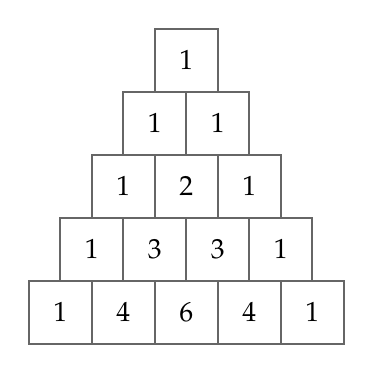
\begin{tikzpicture}[scale=0.8*\scalefactor]

\newcommand{\trisquare}[3]{

  \draw[align=flush center,text=black!100] (#1+0.5,#2+0.5) node {{\textsc{#3}}};
%  \draw[align=flush center,text=black!50] (#1+0.5,#2+0.5) node {\small #1 #2};

  \draw[black!60,thick] (#1, #2) rectangle (#1+1,#2+1);

%  \begin{scope}
%  \clip (#1+0.5,#2-1.0) rectangle (#1+2.0, #2+1.0+1.0);
%  \draw[black!60,very thick] (#1+0.5,#2+0.5) circle (0.5);
%  \end{scope}
}

\trisquare{0}{0}{1}

\trisquare{-0.5}{-1}{1}
\trisquare{0.5}{-1}{1}

\trisquare{-1.0}{-2}{1}
\trisquare{-0.0}{-2}{2}
\trisquare{1.0}{-2}{1}

\trisquare{-1.5}{-3}{1}
\trisquare{-0.5}{-3}{3}
\trisquare{0.5}{-3}{3}
\trisquare{1.5}{-3}{1}

\trisquare{-2.0}{-4}{1}
\trisquare{-1.0}{-4}{4}
\trisquare{-0.0}{-4}{6}
\trisquare{1.0}{-4}{4}
\trisquare{2.0}{-4}{1}



\end{tikzpicture}

\mycaption{A Pascal triangle.\label{triangle}}
\end{figure}




\p{pascal-1}%
Write a program which takes as input a nonnegative
integer $n$ and returns the first $n$ rows of Pascal's triangle.
%Your solution must use $\mathcal{O}(n)$ space.




\autohint{LABELS_REMOVED}{Write the given fact as an equation.}

%dummy for rstrip
\ansbegin{pascal-1}
\label{solution-pascal-1}
%_TODO(THL): Instead of saying following sentence, how about we say something like case analysis which starting from small examples to match the beginning of the next paragraph.
%There is not much scope for algorithm design in this problem---it is predominantly
%about a clean implementation.
A brute-force approach might be to organize the arrays in memory similar
to how they appear in the figure. The challenge is to determine the
correct indices to range over and to read from.

A better approach is to keep the arrays left-aligned, that is
the first entry is at location~$0$. Now it is simple: the $j$th
entry in the $i$th row is $1$ if $j=0$ or $j=i$, otherwise it is
the sum of the $(j-1)$th and $j$th entries in the $(i-1)$th row.
%Since after we complete computing $A^j$, we do not need the results
%for $A^{j-1}$ and earlier to compute $A^{j}$, we can recycle storage.
The first row $R_0$ is $\langle 1\rangle$. The second row $R_1$
is $\langle 1, 1\rangle$.  The third row $R_2$ is $\langle 1, R_1[0] + R_1[1] = 2, 1\rangle$.
The fourth row $R_3$ is $\langle 1, R_2[0] + R_2[1] = 3, R_2[1] + R_2[2] = 3, 1\rangle$.
%_TODO(THL): rewrite this code to make more understandable
\ifCpp
\begin{lstlisting}[language={[11]C++}]
vector<vector<int>> GeneratePascalTriangle(int num_rows) {
  vector<vector<int>> pascal_triangle;
  for (int i = 0; i < num_rows; ++i) {
    vector<int> curr_row;
    for (int j = 0; j <= i; ++j) {
      // Sets this entry to the sum of the two above adjacent entries if they
      // exist.
      curr_row.emplace_back(0 < j && j < i
                                ? pascal_triangle.back()[j - 1] +
                                      pascal_triangle.back()[j]
                                : 1);
    }
    pascal_triangle.emplace_back(curr_row);
  }
  return pascal_triangle;
}
\end{lstlisting}
\fi%ifCpp
\ifJava
\begin{lstlisting}[language=Java]
public static List<List<Integer>> generatePascalTriangle(int numRows) {
  List<List<Integer>> pascalTriangle = new ArrayList<>();
  for (int i = 0; i < numRows; ++i) {
    List<Integer> currRow = new ArrayList<>();
    for (int j = 0; j <= i; ++j) {
      // Set this entry to the sum of the two above adjacent entries if they
      // exist.
      currRow.add((0 < j && j < i)
                      ? pascalTriangle.get(i - 1).get(j - 1)
                            + pascalTriangle.get(i - 1).get(j)
                      : 1);
    }
    pascalTriangle.add(currRow);
  }
  return pascalTriangle;
}
\end{lstlisting}
\fi%ifJava
\ifPython
\begin{lstlisting}[language=Python]
def generate_pascal_triangle(n):
    result = [[1] * (i + 1) for i in range(n)]
    for i in range(n):
        for j in range(1, i):
            # Sets this entry to the sum of the two above adjacent entries.
            result[i][j] = result[i - 1][j - 1] + result[i - 1][j]
    return result
\end{lstlisting}
\fi%ifPython
Since each element takes $\mathcal{O}(1)$
time to compute, the time complexity is $\mathcal{O}(1 + 2 + \dots + n)
= \mathcal{O}(n(n+1)/2) = \mathcal{O}(n^2)$.
Similarly, the space complexity is $\mathcal{O}(n^2)$.

%_TODO(AA): do we need this?
It is a fact that the $i$th entry in the $n$th row of Pascal's triangle
is $\binom{n}{i}$. This in itself does not trivialize the
problem, since computing $\binom{n}{i}$ itself is tricky.
(In fact, Pascal's triangle can be used to compute $\binom{n}{i}$.)

\variant{Compute the $n$th row of Pascal's triangle using $\mathcal{O}(n)$ space.}

\ansend

%_TODO(THL, 1.5): decides the location of this problem in graph chapter.  Check my move of this problem.  Rewrite is probably needed.
%AA: challenging, since it's not graph search, which all but 2 of following are (remaining 2 are shortest path).
%THL: That is the reason I put this before graph search.
%AA: but it's a bad problem to lead off with, since it's not very representative. maybe keep right before adv graph algos?
%_TODO(AA,blocking): i dont like this to lead off graphs, it's not common problem, not a nice problem either. i would
% move to the back of the graph search, maybe mention graph seach is linear, but you can do better. or we can move to end of
% 2D array, since it really has nothing to do with graphs...
%THL: I think I would like to remove this problem even though you draw a picture for this.
%\indexsection{Identify the celebrity}
%\label{identify-celebrity}
%
%For any two distinct people $a$ and $b$, $a$ may or may not know $b$.
%In the context of this problem, the ``knows'' relation is not necessarily symmetric:
%$a$ may know $b$, but $b$ may not know $a$.
%%The knows relation is anti-reflexive, i.e., $a$ does not know $a$.
%At a party, everyone knows someone else. Now a celebrity joins the party---everyone
%knows him, but he knows no one.
%
%\begin{figure}[thb]
%\centering
%\input{graphics/celebrity}
%\mycaption{\label{celebrity-fig}
%In this example, $A$ knows $B$, $B$ knows $C$, $C$ knows $E$, $E$ knows $A$,
%and $A,B,C,E$ all know $D$, and $D$ knows nobody. Then $D$ is the celebrity, and
%the ``knows'' matrix is as shown, with $0$ denoting false and $1$ denoting true.}
%\end{figure}
%


%\p{identify-celebrity}%
%Let $F$ be an $n \times n$ Boolean \myindex{$2$D array}$2$D array
%representing the ``knows'' relation for $n$ people---$F[a][b]$ is true
%if and only if $a$ knows $b$.  See Figure~\vref{celebrity-fig} for an example.
%It is given that there is a celebrity in the relationships described by $F$.
%Design an algorithm to find the celebrity.
%
%\hint{Iteratively eliminate noncelebrities.}
%
%\ansbegin{identify-celebrity}
%\s{bbs forum}
%The brute-force approach  is to teach for each $i$ if $F[i][j]$ is false
%for all $j$ and $F[j][i]$ is true for all $j$ not equal to $i$.
%Each check takes time $\mathcal{O}(n)$, so the time complexity
%of this approach is $\mathcal{O}(n^2)$.
%
%The key to achieving time efficiency is to
%avoid having to look at all of $F$, which will
%always lead to an $\mathcal{O}(n^2)$ (or worse) time complexity.
%%We can do this by process people in order,
%%and eliminate at least one person from the set with each lookup into $F$.
%To do this we can use the following observation.
%Suppose we check $F[i][j]$ where $i < j$. The problem statement guarantees
%that if $F[i][j]$ is false, $j$ is not the celebrity and $i$ is still a possible celebrity candidate.
%Hence we eliminate $j$ from the set of celebrity candidates and move to $F[i][j+1]$.
%If $F[i][j]$ is true, $i$ cannot be the celebrity, and for all $j' < j$,
%$j'$ is not a celebrity because $F[i][j']$ must be false. We then move to
%$F[j][j+1]$ since $i < j$.
%In essence, we eliminate at least one person from the set with each lookup into $F$.
%We begin by checking $F[0][1]$.
%
%For the given example, we start by looking at $F[A][B]$.
%Since it is true, we know $A$ is not the celebrity. We turn to $F[B][C]$.
%Since it is true, we know $B$ is not the celebrity. We turn to $F[C][D]$.
%Since it is true, we know $C$ is not the celebrity.
%Now we look at $F[D][E]$. Since it's false, it means $D$ does not know anybody.
%Therefore $D$ is the celebrity.
%\codefileinclude{Celebrity_finding.cc}{CelebrityFinding.java}
%Since we eliminate one candidate each step in $\mathcal{O}(1)$
%time the overall algorithm runs in $\mathcal{O}(n)$ time.
%
%%\variant{Solve the same problem when the knows relation is not reflexive, nor anti-reflexive, i.e., some people may know themselves, and others may not.}
%%_TODO(THL): remove this variant since we don't count on reflexive property here.
%
%\ansend

\end{Spacing}


\part{Domain Specific Problems}

\renewcommand{\blueboxheight}{16}
\setlength{\epigraphwidth}{0.48\textwidth}
\renewcommand{\epioffset}{-55mm}
\sixnineEpi{16}{0.48}{-54mm}
\chapter{Common Tools}
\label{chap-tools}
\myepigraph{%
UNIX is a general-purpose, multi-user, interactive
operating system for the Digital Equipment Corporation
PDP-11/40 and 11/45 computers. It offers a number
of features seldom found even in larger operating systems,
including: (1) a hierarchical file system incorporating
demountable volumes; (2) compatible file, device,
and inter-process I/O; (3) the ability to initiate asynchronous
processes; (4) system command language selectable
on a per-user basis; and (5) over 100 subsystems
including a dozen languages.
}
{---~``\textit{The UNIX TimeSharing System},''\\ \textsc{D.~Ritchie and K.~Thompson}, 1974}{\epioffset}

\begin{Spacing}{\commonToolsSpacing}

The problems in this chapter are concerned with tools:
version control systems, scripting languages, build systems,
databases, and the networking stack.
Such problems are not commonly asked---expect them only if you are interviewing for a specialized
role, or
%_TODO(THL): for example of?  This English looks weird to me.
%AA: updated
if you claim specialized knowledge, e.g., network security or databases.
We emphasize these are vast subjects, e.g., networking is taught
as a sequence of courses in a university curriculum. Our goal here
is to give you a flavor of what you might encounter.
Adnan's Advanced Programming Tools course material, available freely
online, contains lecture notes, homeworks, and labs  that may serve
as a good resource on the material in this chapter.

%_TODO(THL): should we call it "Version control system" instead of initial here?
%AA: ok updated, as per wiki
%THL: I am talking about \ds here.
\ds{Version control}

Version control systems are a cornerstone of software development---every developer should understand how to use them in an optimal way.

\indexsection{Merging in a version control system}
\label{semantic-syntax}


\pnovs{semantic-syntax}%
What is merging in a version control system?
Specifically, describe the limitations of line-based merging
and ways in which they can be overcome.


\ansbegin{semantic-syntax}
\label{solution-semantic-syntax}
% List pros and cons for textual, syntactical and semantical integration.
% How can disadvantages of textual integration be avoided?
% (For example, think of comments in source code, or different formatting styles.)
%
% %TODO(THL): it would be great if we can show three concrete examples here of different integrations.
% %TODO(AA): from keith, wrote asking for permission
% \ansbegin{semantic-syntax}
% \begin{itemize}
% \item Textual integration
% \begin{itemize}
% \item Pros: This is the easiest approach.  It is easy to implement since it has stock algorithms.  It is also the fastest in the three approaches since it treats source code as texts.
% \item Cons: It does the least amount of work since it does not consider syntax or program behaviors.  It cannot tell if a change affects the program behaviors or not, e.g. a change in a comment vs. a change in a
% class definition.  Also, if a conflict occurs, the user needs to check every detail to resolve the conflict.
% In this case, this approach does not offer useful information other than textual differences.
% \end{itemize}
% \item Syntactical integration:
% \begin{itemize}
% \item Pros: It is not too hard to implement compared to the semanical integration below.  For example, one possible implementation is to construct two parse trees and compare them by tree traversals.  Also, the user now does not need to worry about conflict caused by simple syntax changes like whitespaces or moving comments around.
% %TODO(THL): space linear? should it be linear space?
% %AA: it's ok
% %TODO(THL): Why you said it is "VC system" instead of "VCS"?
% \item Cons: It is still harder to implement than textual integration, since now the parser comes into play.  It also takes more time since parsing the source code may need several passes.  The comparison of the parse trees also may take space linear in the size of the source code.  If the language specification changes, then the VC must be changed accordingly.  The VC system also needs detailed knowledge of those languages used, e.g. projects using more than one programming languages.  The user still needs to check by hand if a change affects the program behavior.
% \end{itemize}
% \item Semantical integration:
% \begin{itemize}
% \item Pros: The amount of work by the user is greatly reduced.  This approach automates the changes that does not affect program behaviors, i.e. same semantics.
% %TODO(THL): what is PSPACE-complete, should we mention it is like Go?
% %AA: just said it's hard
% \item Cons: It is the hardest approach to implement.  To ensure the semantics are still the same, the VC system may need program validation or software testing to ensure two sematics are equivalent.  This takes huge amount of time and space.  For example, it is known that deciding the equivalence of two regular expressions
% has very high complexity.
% % is PSPACE-complete.
% So the VC system needs huge resources for a simple change in the pattern matching, even if the two patterns can be checked equivalent by human eye.  Also, in a centralized VC system, the server may need to simultaneously perform several program validation or software testing for multiple clients, which is not practical if the team has more than a dozen of developers.  Furthermore, if a project uses more than one programming languages, the VC system needs knowledge of the specifications of several programming language.
% \end{itemize}
% \end{itemize}
% To avoid the disadvantages of textual integration, the VC system may consider the specifications of the languages of the source code.  For example, in C++ or Java, it can safely skip multiple adjacent semicolons, or skip whitespaces between the last semicolon and the start of next line.  The VC system may also utilize annotations (e.g. Javadoc).  For example, it may use annotations to identify method signatures.  So when a user changes the parameter names of a method, the VC will utilize this information to resolve conflicts (if there is one).

%AA: from chrome-extension://mloajfnmjckfjbeeofcdaecbelnblden/https://hiper.cis.udel.edu/lp/lib/exe/fetch.php/courses/cisc879/survey_software_merging.pdf, completely rewritten

Modern version control systems allow developers to work concurrently
on a personal copy of the entire codebase. This allows
software developers to work
independently. The price for this merging: periodically, the personal copies
need to be integrated to create a new shared version.
There is the possibility that parallel changes are conflicting,
and these must be resolved during the merge.


By far, the most common approach to merging is text-based.
Text-based merge tools view software as text. Line-based
merging is a kind of text-based merging, specifically
one in which each line is treated as an indivisible unit.
The merging is ``three-way'': the lowest common ancestor in the revision history
is used in conjunction with the two versions.
With line-based merging of text files, common text lines
can be detected in parallel modifications, as well as text
lines that have been inserted, deleted, modified, or moved.
Figure~\vref{integration-vcs} shows an example of such a line-based merge.

One issue with line-based merging is that
it cannot handle two parallel modifications to the same line:
the two modifications cannot be combined,
only one of the two modifications must be selected.
A bigger issue is that a line-based merge may succeed, but the resulting
program is broken because of syntactic or semantic conflicts.
In the scenario in Figure~\vref{integration-vcs} the changes
made by the two developers are made to independent lines, so the line-based
merge shows no conflicts. However, the program will not compile because a function
is called incorrectly.

In spite of this, line-based merging is widely used
because of its efficiency, scalability,and accuracy.
A three-way, line-based merge tool in practice will merge
90\% of the changed files without any issues. The challenge is to automate
the remaining 10\% of the situations that cannot be merged automatically.

Text-based merging fails
because it does not
consider any syntactic or semantic information.

Syntactic merging takes the syntax of the programming language
into account. Text-based merge often
yields unimportant conflicts such as a code comment
that has been changed by different developers or
conflicts caused by  code reformatting.
A syntactic merge can ignore all these:
it displays a merge conflict when the merged result is not syntactically correct.

We illustrate syntactic merging with a small example:
\begin{lstlisting}
if (n%2 == 0) then m = n/2;
\end{lstlisting}
Two developers change this code in a different ways,
but with the same overall effect. The first updates it to
\begin{lstlisting}
if (n%2 == 0) then m = n/2 else m = (n-1)/2;
\end{lstlisting}
and the second developer's update is
\begin{lstlisting}
m = n/2;
\end{lstlisting}
Both changes to the same thing. However, a textual-merge will likely result in
\begin{lstlisting}
m := n div 2 else m := (n-1)/2
\end{lstlisting}
which is syntactically incorrect. Syntactic merge identifies the conflict; it is the
integrator's responsibility to manually resolve it, e.g., by
removing the \verb+else+ portion.

Syntactic merge tools are unable to detect some frequently occurring conflicts. For example, in
the merge of Versions {\em 1a} and {\em 1b} in Figure~\vref{integration-vcs}
will not compile, since  the call to \verb+sum(10)+ has the wrong signature.
Syntactic merge will not detect this conflict
since the program is still syntactically correct. The conflict is
a semantic conflict, specifically, a static semantic conflict, since
it is detectable at compile-time. (The compile will return something like
``function argument mismatch error''.)

% Observe that the merge of Versions {\em 1a} and {\em 1b} contains a second semantic problem.
% Line 15 contains a procedure call \verb+fac(5,R);+
% while the procedure definition has been replaced by a
% function definition \verb+func fac(arg:int):int+ on Line 4.
% Obviously, these two changes at different locations in the code are incompatible and give
% rise to an error when the merged program is compiled.
% Tree-based merge approaches based on parse trees cannot detect
% this kind of conflict because the relationship
% between procedure (or function) definition and procedure(or function) invocation
% is not made explicit in a parse tree or abstract syntax tree.
% Graph-based merge approaches can detect this conflict because a graph representation
% maintains an explicit link between a definition and its
% invocations, thus making it easy to detect incompatibilitiesbetween them.

Technically, syntactic merge algorithms operate on the parse trees of the programs
to be merged. More powerful static semantic merge algorithms have been proposed that
operate on a graph representation of the programs, wherein definitions and usage are
linked, making it easier to identify mismatched usage.

Static semantic merging also has shortcomings.  For example, suppose \texttt{Point}
is a class representing $2D$-points using Cartesian coordinates,
and that this class has a distance function that returns $\sqrt{x^2 + y^2}$.
Suppose Alice checks out the project, and subclasses \texttt{Point} to create a class that supports polar coordinates,
and uses \texttt{Points}'s distance function to return the radius.
Concurrently, Bob checks out the project and changes \texttt{Point}'s distance function to return $|x| + |y|$.
Static semantic merging reports no conflicts: the merged program compiles without any trouble.
However the behavior is not what was expected.
%because independent changes by parallel developers may
%still give rise to unexpected behavior in the merged result.
%Indeed, one has no guarantees about how the execution
%behavior of the merged program relates to the behavior of
%the programs being merged. The resulting
%behavioral conflictscan only be countered by resorting to even
%more sophisticated semantic merge techniques that rely on the runtime semantics of the code.

Both syntactic merging and semantic merging greatly increase runtimes, and
are very limiting since they are tightly coupled to specific programming languages.
In practice, line-based merging is used in conjunction with
a small set of unit tests (a ``smoke suite'') invoked with
a pre-commit hook script. Compilation finds syntax and static semantics
errors, and the tests (hopefully) identify deeper semantic issues.


%\begin{figure}
%\centering
%\includegraphics[width=0.6\textwidth]{graphics/integration-vcs.png}
%\mycaption{Integration in a VCS.\label{integration-vcs}}
%\end{figure}

\begin{figure}[hbt]
\centering
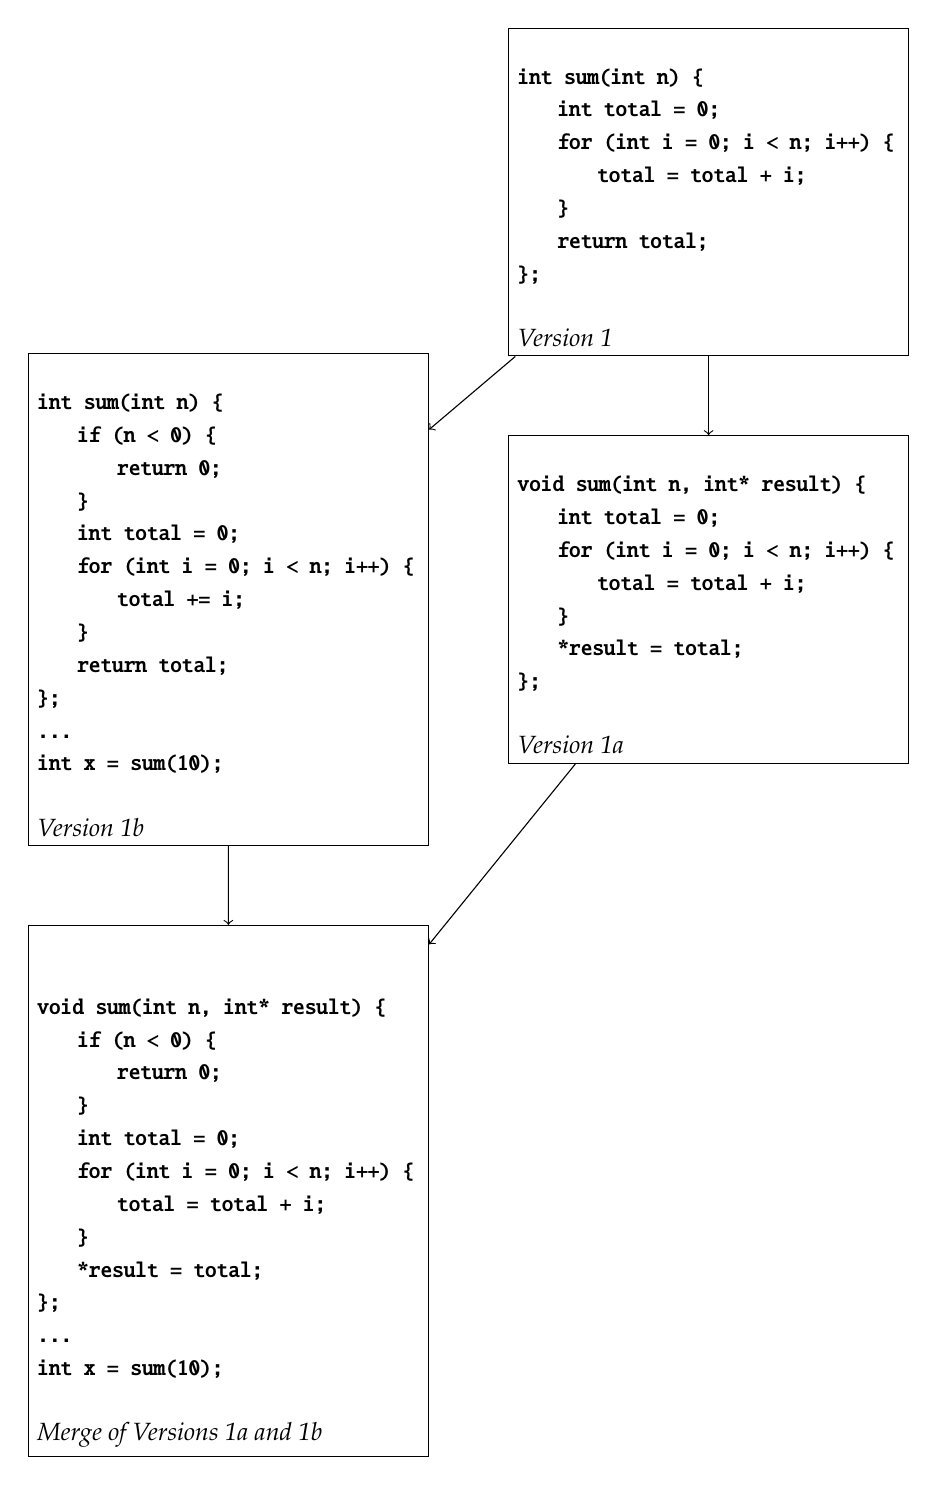
\begin{tikzpicture}[scale=0.3]
{
\lstset{
%frame=tb,
  language=C++,
  aboveskip=3mm,
  belowskip=3mm,
  showstringspaces=false,
  columns=flexible,
  %basicstyle={\small\ttfamily},
  basicstyle=\ttfamily\footnotesize\bfseries,
  numbers=none,
  numberstyle=\tiny\color{gray},
  %keywordstyle=\color{blue},
  commentstyle=\color{dkgreen},
  %stringstyle=\color{mauve},
  breaklines=true,
  breakatwhitespace=true,
  tabsize=3
}

\usetikzlibrary{positioning}

\tikzset{
  big blue arrow/.style={
    decoration={markings,mark=at position 1 with {\arrow[scale=4,blue]{>}}},
    postaction={decorate},
    shorten >=0.4pt}
}


\node(listing1)[draw]{%
\begin{minipage}{.40\linewidth}
\begin{lstlisting}
int sum(int n) {
    int total = 0;
    for (int i = 0; i < n; i++) {
        total = total + i;
    }
    return total;
};
\end{lstlisting}
{\small \em Version 1}
\end{minipage}
}
node(listing3)[draw,below=of listing1]{%
\begin{minipage}{.40\linewidth}
\begin{lstlisting}
void sum(int n, int* result) {
    int total = 0;
    for (int i = 0; i < n; i++) {
        total = total + i;
    }
    *result = total;
};
\end{lstlisting}
{\small \em Version 1a}
\end{minipage}
}
node(listing2)[draw,below=of listing1,left=of listing3]{%
\begin{minipage}{.40\linewidth}
\begin{lstlisting}
int sum(int n) {
    if (n < 0) {
        return 0;
    }
    int total = 0;
    for (int i = 0; i < n; i++) {
        total += i;
    }
    return total;
};
...
int x = sum(10);
\end{lstlisting}
{\small \em Version 1b}
\end{minipage}
}
node(listing4)[draw,below=of listing2]{%
\begin{minipage}{.40\linewidth}
\begin{lstlisting}

void sum(int n, int* result) {
    if (n < 0) {
        return 0;
    }
    int total = 0;
    for (int i = 0; i < n; i++) {
        total = total + i;
    }
    *result = total;
};
...
int x = sum(10);
\end{lstlisting}
{\small \em Merge of Versions 1a and 1b}
\end{minipage}
};

\draw[->] (listing1)--(listing2);
\draw[->] (listing1)--(listing3);
\draw[->] (listing2)--(listing4);
\draw[->] (listing3)--(listing4);
}

\end{tikzpicture}

\mycaption{An example of a 3-way line based merge. \label{integration-vcs}}
\end{figure}
\ansend

\indexsection{Hooks}
\label{commit-hooks}



\pnovs{commit-hooks}%
What are hooks in a version control system? Describe their applications.


\ansbegin{commit-hooks}
\label{solution-commit-hooks}
%Version control systems such as git and SVN expose a number of integration points
%called hooks into the transaction lifecycles.
Version control systems such as git and SVN allow users to define actions to take around events such as commits,
locking and unlocking files, and altering revision properties.
These actions are specified as executable programs known as hook scripts.
When the version control system gets to these events, it
will check for the existence of a corresponding hook
script, and execute it if it exists.

Hook scripts have access to the action as it is taking place,
and are passed corresponding command-line arguments.
For example, the pre-commit hook is passed the
repository path and the transaction ID for the currently executing commit.
If a hook script returns a nonzero exit code, the version control system aborts
the action, returning the script's standard error output to the user.

The following hook scripts are used most often:
\begin{itemize}
\item {\em pre-commit:} Executed before a change is committed to the repository.
Often used to check log messages, to format files, run a test suite, and to
perform custom security or policy checking.
\item {\em post-commit:} Executed once the commit has completed. Often used to
inform users about a completed commit, for example by sending an email to
the team, or update the bug tracking system.
\end{itemize}
As a rule, hooks should never  alter the content of the transaction. At the very
least, it can surprise a new developer; in the worst-case, the change can result
in buggy code.
\ansend

\ds{Database}

Most software systems today interact with databases, and it's important
for developers to have basic knowledge of databases.

%_TODO(THL): Change the name to SQL vs. NoSQL?
\indexsection{SQL vs.~NoSQL}
\label{nosql}


\pnovs{nosql}%
Contrast SQL and NoSQL databases.


\ansbegin{nosql}
\label{solution-nosql}
A relational database is a set of tables (also known as relations).
Each table consists of rows.
A row is a set of columns (also known as fields or attributes), which
could be of various types (integer, float, date, fixed-size string, variable-size string, etc.).
SQL is the language used to create and manipulate such databases.
MySQL is a popular relational database.

A NoSQL database provides a mechanism for storage and retrieval of
data which is modeled by means other than
the tabular relations used in relational databases.
MongoDB is a popular NoSQL database.
The analog of a table in MongoDB is a collection, which consists of documents.
Collections do not enforce a schema. Documents can be viewed as
hash maps from fields to values. Documents within a collection can have different fields.

A key benefit of NoSQL databases is simplicity of design: a field
can trivially be added to new documents in a collection without this affecting
documents already in the database. This makes NoSQL a popular choice
for startups which have an agile development environment.

The data structures used by NoSQL databases,
e.g., key-value pairs in MongoDB,
are different from those used by default in relational databases, making
some operations faster in NoSQL.
NoSQL databases are typically much simpler to scale
horizontally, i.e., to spread documents from a collection across a cluster of machines.

A key benefit of relational databases include support for ACID transactions. ACID
(Atomicity, Consistency, Isolation, Durability) is a
set of properties that guarantee that database transactions are processed reliably.
For example, there is no way in MongoDB to remove an
item from inventory and add it to a customer's order as an atomic operation.

Another benefit of relational database is that their query language, SQL, is
declarative, and relatively simple. In contrast, complex queries
in a NoSQL database have to be implemented programmatically. (It's often
the case that the NoSQL database will have some support for translating
SQL into the equivalent NoSQL program.)
\ansend

\indexsection{Normalization}
\label{db-normalization}



\pnovs{db-normalization}%
What is database normalization? What are its advantages and disadvantages?


\ansbegin{db-normalization}
\label{solution-db-normalization}
Database normalization is the process of organizing the columns and
tables of a relational database to minimize data redundancy.
Specifically, normalization involves decomposing a table into less redundant
tables without losing information,
thereby enforcing integrity and saving space.

The central idea is the use of ``foreign keys''.
\label{foreign-key}
A foreign key is a field (or collection of fields) in one table that
uniquely identifies a row of another table.
In simpler words, the foreign key is defined in a second table, but it refers to the unique
key in the first table.
For example, a table called Employee may use a unique
key called employee\_id. Another table called Employee Details has a foreign key
which references employee\_id in order to uniquely identify the relationship
between both the tables.
The objective is to
isolate data so that additions, deletions, and modifications of an
attribute can be made in just one table and then propagated through
the rest of the database using the defined foreign keys.

The primary drawback of normalization is performance---often, a
large number of joins are required
to recover the records the application needs to function.
\ansend

\indexsection{SQL design}
\label{sql-design}

%You have to create a database for student grades.
%Specifically, write a SQL query
%that returns the top $k$ students averaged over their $h$ highest test scores?
%A student who has fewer than $h$ test scores should not be included
%in the calculation. All tests are on 100.
%How would you optimize the database for such queries?
%How would you have this result continuously updated as new scores are added? (Trigger)



\pnovs{sql-design}%
Write SQL commands to create a table appropriate for
representing students as well as SQL commands that
illustrate how to add, delete, and update students, as well
as search for students by
GPA with results sorted by GPA.

Then add a table of faculty advisors, and describe how to
model adding an advisor to each student. Write a SQL query that
returns the students who have an advisor with a specific name.

%_TODO(THL): Why called it gpa instead of GPA?

\ansbegin{sql-design}
\label{solution-sql-design}
Natural fields for a student are name, birthday, GPA, and graduating
year. In addition, we would like a unique key to serve as an identifier.
A SQL statement to create a student table would look like the following:
\texttt{CREATE TABLE students (id INT AUTO\_INCREMENT, name VARCHAR(30), birthday DATE, gpa FLOAT, graduate\_year INT, PRIMARY KEY(id));}.
Here are examples of SQL statements for updating the students table.
\begin{itemize}
\item Add a student
\begin{itemize}
%_TODO(THL): is following command correct that fields do not match exactly?  birth vs. birthday and grad vs. graduate_year.  We need carful check of this problem.
\item \texttt{INSERT INTO students(name, birthday, gpa, graduate\_year) VALUES ('Cantor', '1987-10-22', 3.9, 2009);}
\end{itemize}
\item Delete students  who graduated before 1985.
\begin{itemize}
\item \texttt{DELETE FROM students WHERE graduate\_year < 1985;}
\end{itemize}
%_TODO(THL): add respectively to the end?
\item Update the GPA and graduating year of the student with id 28 to 3.14 and 2015, respectively.
\begin{itemize}
\item \texttt{UPDATE students SET gpa = 3.14, graduate\_year = 2015 WHERE id = 28;}
\end{itemize}
\end{itemize}

The following query returns students with a GPA greater than $3.5$, sorted by GPA.
It includes each student's name, GPA, and graduating year.
\texttt{SELECT gpa, name, graduate\_year FROM students WHERE gpa > 3.5 ORDER BY gpa DESC;}

Now we turn to the second part
of the problem. Here is a sample table for faculty advisers.
%_TODO(THL): let' try to centralzie verbatim figures as it looks a little weird in 7 * 10 setting.
\begin{center}
\begin{tabular}{|lll|} \hline
{\em id} &  {\em name} & {\em title} \\
1 & Church & Dean \\
2 & Tarski & Professor \\
\hline
\end{tabular}
\end{center}
%\end{tabular}
%\begin{verbatim}
%+----+----------+-----------+
%| id | name     | title     |
%+----+----------+-----------+
%|  1 | Fujimura | assocprof |
%|  2 | Bolosky  | prof      |
%+----+----------+-----------+
%\end{verbatim}

We add a new column advisor\_id to the students table. This is the foreign key~\vpageref{foreign-key}.
As an example, here's how to return students with GPA whose advisor is Church:
\texttt{SELECT s.name, s.gpa FROM students s, advisors p WHERE s.advisor\_id = p.id AND p.name = 'Church';}.

\variant{What is a SQL join? Suppose you have a table of courses
and a table of students. How might a SQL join arise naturally in such a database?}

\ansend

\end{Spacing}

%_TODO(THL, 1.5): chapter title and epitgraph.
%The path to greatness
% what doesnt kill you makes you stronger
% these are all asked
% all quite challenging
% make you very very strong if you solve them (but not essential to sucess)
% specialized knowledge/background: prob, graphs
% just challenging yourself
% quote from darwin or from nietzche
% study guide: 10 favorites, start with these
% bounce around
% asked nina -> you are very good, can have huge payoff
% mention keep positive in strategies for a great interview
\part{The Honors Class}

\renewcommand{\blueboxheight}{12}
\setlength{\epigraphwidth}{0.42\textwidth}
\sixninepigraphwidth{0.50}
\renewcommand{\epioffset}{-34.5mm}
\sixnineEpi{12}{0.42}{-34.5mm}
\chapter{Honors Class}
\label{chap-ninja}

\myepigraph{%
The supply of problems in mathematics is inexhaustible, and as soon as one problem
is solved numerous others come forth in its place.
}
{---~``\textit{Mathematical Problems},''\\ \textsc{D.~Hilbert}, 1900}{\epioffset}
%_TODO(THL): where the paper and came from, just curious?  BTW, how about drop "The"?

\begin{Spacing}{\honorsSpacing}

\noindent
This chapter contains problems that are more difficult to solve than the ones presented earlier.
Many of them are commonly asked at interviews, albeit with the
expectation that the candidate will not deliver the best solution.

There are several reasons why we included these problems:
\begin{itemize}
\item Although mastering these problems is not essential
to your success, if you do solve them, you will have put yourself into a very strong
position, similar to training for a race with ankle weights.
\item If you are asked one of these questions or a variant thereof, and you successfully derive the best
solution, you will have strongly impressed your interviewer.
The implications of this go beyond being made
an offer---your salary, position, and status will all go up.
%\item You are more likely to encounter them if you have a graduate degree.
\item Some of the problems
are appropriate for candidates interviewing for specialized positions, e.g., optimizing large scale distributed systems,
machine learning for computational finance, etc. They are also commonly asked of
candidates with advanced degrees.
\item Finally, if you love a good challenge, these problems will provide it!
\end{itemize}
You should be happy if your interviewer asks you a hard question---it implies high expectations, and
is an opportunity to shine, compared, for example,
to being asked to write a program that tests if a string is palindromic.

%epilight-skip-begin
Problems roughly follow the sequence of topics of the previous chapters, i.e., we begin with primitive
types, and end with graphs.
We recommend you solve these problems in a randomized order.
%TODO(AA): demath/deitorialize these first
The following problems are a good place to begin with:~Problems \ref{gcd}, \ref{rotate-string}, \ref{format-text}, \ref{reorder-list}, \ref{moving-window}, \ref{bt-traversal}, \ref{max-line}, \ref{sorted-list-2-BST}, \ref{2d-render}, \ref{grep}, \ref{max-boolean-submatrix}.
White ninja (\ninjawhite{0.08}) problems are though challenging, should be solvable
by a good candidate given enough time.
Black ninja (\ninjablack{0.08}) problems are exceptionally difficult, and
are suitable for testing a candidate's response to stress, as described on~Page\pageref{stress-interview}.
%THL's choice: rotate-string,justify text, copy-postings-list,maximum-sliding-window,preorder and postorder without recursions, line through most points,sorted doubly linked list to bst,grep, view from above,minimum delay and unlimited resources.
%epilight-skip-end

%common: rotate-string, list to BST, grep
%agree: gcd, max-sliding-window, preorder and postorder without recursions, minimum delay and unlimited resources, view from above,
% line through most points, rw-3, justify-text, max-2d-subarray, list-zipping

\section*{Intractability}
Coding problems asked in interviews almost always have one (or more)
solutions that are fast, e.g., $\mathcal{O}(n)$ time complexity.
Sometimes, you may be asked a problem that is computationally intractable---there may
not exist an efficient algorithm for it. (Such problems are common
in the real world.)
%Complexity theory
%addresses these problems. Some have been proved to not have an efficient solution
%%(such as checking the validity of a certain class of formulas expressing relationships
%% involving $\exists, +,<, \Rightarrow$ on the integers)
%but the vast majority are only
%conjectured to be intractable.
%The \myindex{conjunctive normal form satisfiability|see{CNF-SAT}}conjunctive normal form satisfiability (\myindex{CNF-SAT|textbf}CNF-SAT) problem is an example of a
%problem that is conjectured to be intractable.
%Specifically, the \myindex{CNF-SAT}CNF-SAT problem belongs to the
%complexity class \myindex{NP|textbf}NP---problems for which a candidate solution
%can be efficiently checked---and is conjectured to be the hardest problem in this class.
%When faced with a problem $P$ that appears to be intractable,
%the first thing to do is to prove \myindex{intractability}intractability.
%This is usually done by taking a problem which is known to be intractable and showing how it can be efficiently reduced to $P$.
%Often this reduction gives insight into the cause of \myindex{intractability}intractability.
%
%Unless you are a complexity theorist,
%proving a problem to be intractable is only the starting point.
%Remember something is a problem only if it has a solution.
There are a number of approaches to solving intractable problems:
\label{coping-with-intractability}
\begin{itemize}
%\itemsep 1pt
\item brute-force solutions, including dynamic programming,
which have exponential time complexity, may be acceptable, if the instances encountered are small,
or if the specific parameter that the complexity is exponential in is small;
\item search algorithms, such as backtracking, branch-and-bound, and hill-climbing,
which prune much of the complexity of a brute-force search;
\item \myindex{approximation algorithm}approximation algorithms which return a solution that is provably close to optimum;
\item heuristics based on insight, common \myindex{case analysis}case analysis, and careful tuning that may solve the problem reasonably well;
\item \myindex{parallel algorithm}parallel algorithms, wherein a large number of computers can work on subparts simultaneously.
\end{itemize}
%_TODO(AA): reorder in right sequence
%Solutions
%\vref{solution-string-dictionary},
%\vref{solution-collatz},
%%\vref{solution-facility-location},
%\vref{solution-sudoku-solver},
%\vref{solution-operators-string},
%\vref{solution-01knapsack},
%\vref{solution-three-jugs}, and
% \vref{solution-min-subarray-difference},
%\vref{solution-tsp},
%\vref{solution-big-sort}
%illustrate the use of some of these techniques.

%---ninja storm
\starindexsection{Compute the greatest common divisor}
\label{gcd}
\myindex{divisor!greatest common divisor}

The \myindex{greatest common divisor|see{GCD}}greatest common divisor (\myindex{GCD|textbf}GCD) of nonnegative integers $x$ and $y$ is the largest integer $d$ such that
$d$ divides $x$ evenly, and $d$ divides $y$ evenly, i.e., $x \bmod d = 0$ and $y \bmod d = 0$. (When
both $x$ and $y$ are $0$, take their GCD to be $0$.)

\widowpenalty=10000


\p{gcd}%
Design an efficient algorithm for computing the \myindex{GCD}GCD of two nonnegative integers
without using multiplication, division or the modulus operators.




\autohint{LABELS_REMOVED}{Use \myindex{case analysis}case analysis: both even; both odd; one even and one odd.}

%dummy for rstrip
\ansbegin{gcd}
\label{solution-gcd}
The straightforward algorithm is based on recursion.
If $x=y$, $\mbox{GCD}(x,y) = x$; otherwise, assume without loss of generality,
that $x > y$. Then $\mbox{GCD}(x,y)$ is the $\mbox{GCD}(x-y,y)$.

The recursive algorithm based on the above does not use multiplication, division or modulus,
but for some inputs it is very slow. %---its time complexity is $\mathcal{O}(\max(x,y))$, which is exponential
%in the size of the input. (Expressed in binary, the numbers $x$ and $y$,
%require $\lceil \log x\rceil$ and $\lceil \log y\rceil$ bits respectively.)
As an example, if the input is $x=2^n$, $y=2$, the algorithm makes
$2^{n-1}$ recursive calls.
The time complexity can be improved by observing
that the repeated subtraction amounts to division, i.e.,
when $x>y$, $\mbox{GCD}(x,y)$ = $\mbox{GCD}(y, x \bmod y)$, but this approach uses integer division
which was explicitly disallowed in the problem statement.

Here is a fast solution, which is also based on \myindex{recursion}recursion, but
does not use general multiplication or division. Instead it uses case-analysis,
specifically, the cases of one, two, or none of the numbers being even.
\myindex{case analysis}

An example is illustrative. Suppose we were to compute the GCD of
$24$ and $300$. Instead of repeatedly subtracting $24$ from $300$, we
can observe that since both are even, the result is $2\times \mbox{GCD}(12,150)$.
Dividing by $2$ is a right shift by $1$, so
we do not need a general division operation. Since $12$ and $150$ are both
even, $\mbox{GCD}(12,150)= 2\times \mbox{GCD}(6,75)$.
Since $75$ is odd, the GCD of $6$ and $75$ is the same as
the GCD of $3$ and $75$, since $2$ cannot divide $75$.
The GCD of $3$ and $75$ is the GCD of $3$ and $75-3  = 72$.
Repeatedly applying the
same logic, $\mbox{GCD}(3,72) = \mbox{GCD}(3,36) = \mbox{GCD}(3,18) = \mbox{GCD}(3,9) = \mbox{GCD}(3,6) = \mbox{GCD}(3,3) = 3$.
This implies $\mbox{GCD}(24,300) = 2 \times 2 \times 3 = 12$.

More generally, the base case is when the two arguments
are equal, in which case the GCD is
that value, e.g., $\mbox{GCD}(12,12) = 12$,
or one of the arguments is zero, in which case the other is the GCD,
e.g., $\mbox{GCD}(0,6) = 6$.

Otherwise, we check if none, one, or both numbers are even. If both
are even, we compute the \myindex{GCD}GCD of the halves of the original numbers, and return
that result times $2$; if exactly one is even, we half it, and return the \myindex{GCD}GCD of
the resulting pair; if both are odd, we subtract the smaller from the larger
and return the \myindex{GCD}GCD of the resulting pair.
Multiplication by $2$ is trivially implemented with a single left shift.
Division by $2$ is done with a single right shift.


%_TODO(THL): remove biginteger to simplify the code.
%Languages such as Java and Python include libraries for manipulating integers
%of arbitrary length, making them ideally suited for our application.
%_TODO(THL, blocking): should we discuss the case if x == 0 or y == 0.
\ifCpp
\begin{lstlisting}[language={[11]C++}]
long long GCD(long long x, long long y) {
  if (x > y) {
    return GCD(y, x);
  }
  if (x == y) {
    return x;
  } else if (x == 0) {
    return y;
  } else if (!(x & 1) && !(y & 1)) {  // x and y are even.
    return GCD(x >> 1, y >> 1) << 1;
  } else if (!(x & 1) && y & 1) {  // x is even, and y is odd.
    return GCD(x >> 1, y);
  } else if (x & 1 && !(y & 1)) {  // x is odd, and y is even.
    return GCD(x, y >> 1);
  }
  return GCD(x, y - x);  // Both x and y are odd.
}
\end{lstlisting}
\fi%ifCpp
\ifJava
\begin{lstlisting}[language=Java]
public static long GCD(long x, long y) {
  if (x > y) {
    return GCD(y, x);
  } else if (x == 0) {
    return y;
  } else if ((x & 1) == 0 && (y & 1) == 0) { // x and y are even.
    return GCD(x >>> 1, y >>> 1) << 1;
  } else if ((x & 1) == 0 && (y & 1) != 0) { // x is even, y is odd.
    return GCD(x >>> 1, y);
  } else if ((x & 1) != 0 && (y & 1) == 0) { // x is odd, y is even.
    return GCD(x, y >>> 1);
  }
  return GCD(x, y - x); // Both x and y are odd.
}
\end{lstlisting}
\fi%ifJava
\ifPython
\begin{lstlisting}[language=Python]
def gcd(x, y):
    if x > y:
        return gcd(y, x)
    elif x == 0:
        return y
    elif not x & 1 and not y & 1:  # x and y are even.
        return gcd(x >> 1, y >> 1) << 1
    elif not x & 1 and y & 1:  # x is even, y is odd.
        return gcd(x >> 1, y)
    elif x & 1 and not y & 1:  # x is odd, y is even.
        return gcd(x, y >> 1)
    return gcd(x, y - x)  # Both x and y are odd.
\end{lstlisting}
\fi%ifPython
Note that the last step leads to a recursive call with one even and one odd number.
Consequently, in every two calls, we reduce the combined bit length of the two numbers by
at least one, meaning that the time complexity is proportional to the sum of
the number of bits in $x$ and $y$, i.e., $\mathcal{O}(\log x + \log y ))$.
%_TODO(AA): should we include the 2 in the base? also, is this clearer than max?
%THL: We don't include 2 in the base for complexity since it makes no difference, but for noncomplexity usage, we explicitly denote the base. Personally I am find with log x + log y.

\ansend

\starindexsection{Find the first missing positive entry}
\label{first-missing-positive}



\pnovs{first-missing-positive}%
Let $A$ be an array of length $n$.
Design an algorithm to find the smallest positive integer which is not present in $A$.
You do not need to preserve the contents of $A$.
For example, if $A = \langle 3,5,4,-1,5,1,-1\rangle$, the smallest positive integer not present in $A$ is $2$.
%_TODO(AA): example, and replace \neq with english
%_TODO(THL): I don't know it is O(1) space or not..




\autohint{LABELS_REMOVED}{First, find an upper bound for $x$.}

%dummy for rstrip
\ansbegin{first-missing-positive}
\label{solution-first-missing-positive}
A brute-force approach is to sort $A$ and iterate through it looking for the first gap in the entries after we see an entry equal to $0$.
The time complexity is that of sorting, i.e., $\mathcal{O}(n \log n)$.

%_TODO(AA): make it nonnegative, not positive. consider drawing the figure.

Since all we want is the smallest positive number in $A$, we explore
other algorithms that do not rely on sorting. We could store
the entries in $A$ in a hash table $S$ (Chapter~\ref{hash}),
and then iterate through the positive integers $1,2,3,\dots$ looking for the
first one that is not in $S$. The time complexity is $\mathcal{O}(n)$
to create $S$, and then $\mathcal{O}(n)$ to perform the lookups, since we must
find a missing entry by the time we get to $n+1$ as there are only $n$ entries.
Therefore the time complexity is $\mathcal{O}(n)$. The space complexity
is $\mathcal{O}(n)$, e.g., if the entries from $A$ are all distinct positive
integers.

The problem statement gives us a hint which we can use to reduce the space complexity.
Instead of using an external hash table to store the set of positive integers,
we can use $A$ itself. Specifically, if $A$ contains $k$ between $1$ and $n$,
we set $A[k-1]$ to $k$. (We use $k-1$ because we need to use all $n$ entries, including the entry at index $0$, which
will be used to record the presence of $1$.)
Note that we need to save the presence of the existing entry in $A[k-1]$ if it is between $1$ and $n$.
Because $A$ contains $n$ entries,
the smallest positive number that is missing in $A$ cannot be greater than $n+1$.

For example, let $A = \langle 3,4,0,2\rangle$, $n=4$.
we begin by recording the presence of $3$ by writing it in $A[3-1]$; we save the
current entry at index $2$ by writing it to $A[0]$. Now $A = \langle 0,4,3,2\rangle$.
Since $0$ is outside the range of interest, we advance to $A[1]$, i.e., $4$, which is
within the range of interest. We write $4$ in $A[4-1]$, and save the value at that location
to index $1$, and $A$ becomes $\langle 0,2,3,4\rangle$. The value at $A[1]$ already
indicates that a $2$ is present, so we advance. The same holds for $A[2]$ and $A[3]$.

Now we make a pass through $A$ looking for the first index $i$ such that $A[i] \not= i+1$;
this is the smallest missing positive entry, which is $1$ for our example.

%Therefore we can iterate through $A$, and record which
%values from $1$ to $n$ are present by
%writing $A[i]$ to index $A[i]-1$ if $A[i]$ is between $1$ and $n$, inclusive.
%We save the value at index $A[i]-1$ by
%swapping it with the entry at $i$.
%%_TODO(AA): should we say something about how we advance through i?
%If $A[i]$ is negative or greater than $n$, we simply advance $i$.
%We then make a second pass through $A$ searching for the first index $i$ such that $A[i] \not= i+1$,
%which indicates that $i+1$ is absent.
%If all numbers between $1$ and $n$ are present, the smallest missing positive is $n+1$.

%For example, if $A = \langle 3,0,5,-1,1,3\rangle$, $A$ is updated to $\langle
\ifCpp
\begin{lstlisting}[language={[11]C++}]
// A is passed by value argument, since we change it.
int FindFirstMissingPositive(vector<int> A) {
  // Record which values are present by writing A[i] to index A[i] - 1 if A[i]
  // is between 1 and A.size(), inclusive. We save the value at index
  // A[i] - 1 by swapping it with the entry at i. If A[i] is negative or
  // greater than n, we just advance i.
  for (int i = 0; i < A.size(); ++i) {
    while (0 < A[i] && A[i] <= A.size() && A[i] != A[A[i] - 1]) {
      swap(A[i], A[A[i] - 1]);
    }
  }

  // Second pass through A to search for the first index i such that
  // A[i] != i+1, indicating that i + 1 is absent. If all numbers between 1
  // and A.size() are present, the smallest missing positive is A.size() + 1.
  for (int i = 0; i < A.size(); ++i) {
    if (A[i] != i + 1) {
      return i + 1;
    }
  }
  return A.size() + 1;
}
\end{lstlisting}
\fi%ifCpp
\ifJava
\begin{lstlisting}[language=Java]
public static int findFirstMissingPositive(List<Integer> A) {
  // Record which values are present by writing A.get(i) to index A.get(i) - 1
  // if A.get(i) is between 1 and A.size(), inclusive. We save the value at
  // index A.get(i) - 1 by swapping it with the entry at i. If A.get(i) is
  // negative or greater than n, we just advance i.
  for (int i = 0; i < A.size(); ++i) {
    while (0 < A.get(i) && A.get(i) <= A.size()
           && A.get(A.get(i) - 1) != A.get(i)) {
      Collections.swap(A, i, A.get(i) - 1);
    }
  }

  // Second pass through A to search for the first index i such that A.get(i)
  // != i + 1, indicating that i + 1 is absent. If all numbers between 1 and
  // A.size() are present, the smallest missing positive is A.size() + 1.
  for (int i = 0; i < A.size(); ++i) {
    if (A.get(i) != i + 1) {
      return i + 1;
    }
  }
  return A.size() + 1;
}
\end{lstlisting}
\fi%ifJava
\ifPython
\begin{lstlisting}[language=Python]
def find_first_missing_positive(A):
    # Record which values are present by writing A[i] to index A[i] - 1 if
    # A[i] is between 1 and len(A), inclusive. We save the value at index A[i]
    # - 1 by swapping it with the entry at i. If A[i] is negative or greater
    # than n, we just advance i.
    for i in range(len(A)):
        while 1 <= A[i] <= len(A) and A[i] != A[A[i] - 1]:
            A[A[i] - 1], A[i] = A[i], A[A[i] - 1]

    # Second pass through A to search for the first index i such that A[i] !=
    # i+1, indicating that i + 1 is absent. If all numbers between 1 and
    # len(A) are present, the smallest missing positive is len(A) + 1.
    return next((i + 1 for i, a in enumerate(A) if a != i + 1), len(A) + 1)
\end{lstlisting}
\fi%ifPython
The time complexity is $\mathcal{O}(n)$, since we perform a constant amount of work
per entry. Because we reuse $A$, the space complexity is \myindex{$\mathcal{O}(1)$ space}$\mathcal{O}(1)$.
\ansend


\skullindexsection{Buy and sell a stock $k$ times}
\label{max-difference-k}
This problem generalizes the buy and sell problem introduced~\vref{max-difference-intro}.



\p{max-difference-k}%
Write a program to compute the maximum profit that can be made by buying and selling a share $k$ times over a given day range.
Your program takes $k$ and an array of daily stock prices as input.



%\p{max-difference-k}%
%Formally, \vref{max-difference-2} is to compute the maximum value of $(A[j_0] - A[i_0]) + (A[j_1] - A[i_1]) + \dots + (A[j_{k-1}] - A[i_{k-1}])$ subject to $i_0 < j_0 < i_1 < j_1 < \cdots < i_{k-1} < j_{k-1}$.


\ansbegin{max-difference-k}
\label{solution-max-difference-k}
Here is a straightforward algorithm.
Iterate over $j$ from $1$ to $k$ and iterate
through $A$, recording
for each index $i$ the best solution for $A[0,i]$ with $j$ pairs. We store these
solutions in an auxiliary \myindex{array}array of length $n$. The overall time complexity will be $\mathcal{O}(kn^2)$;
by reusing the \myindex{array}arrays, we can reduce the additional space complexity to $\mathcal{O}(n)$.

We can improve the time complexity to $\mathcal{O}(kn)$, and the
additional space complexity to $\mathcal{O}(k)$ as follows.
%Let $T^j_i$ be the maximum profit achievable with $j$ buys and sells before or at $i$.
Define $B^j_i$ to be the most money you can have if you must make $j-1$ buy-sell transactions
prior to $i$ and buy at $i$.
Define $S^j_i$ to be the maximum profit achievable with $j$ buys and sells with the $j$th
sell taking place at $i$. Then the following mutual recurrence holds:
\begin{eqnarray*}
S^j_i & = & A[i] + \max_{i'<i}{B^{j}_{i'}} \\
B^j_i & = & \max_{i'<i}{S^{j-1}_{i'}} - A[i]
\end{eqnarray*}
%Furthermore, $T^j_i = \max{i'\leq i} S^j_i'$.

The key to achieving an $\mathcal{O}(kn)$ time
bound is the observation that computing $B$ and $S$
requires computing $\max_{i'<i}B^{j-1}_{i'}$ and $\max_{i'<i}S^{j-1}_{i'}$. These two
quantities can be computed in constant time for each $i$ and $j$ with a conditional update.
In code:
%_TODO(THL, 1.5): This code is still problematic if I change it to double. Need investigate on that.
%TODO(AA): THL rewrote the program to a easy to understand way, lets rewrite this problem.
\ifCpp
\begin{lstlisting}[language={[11]C++}]
double MaxKPairsProfits(const vector<double> &prices, int k) {
  if (!k) {
    return 0.0;
  } else if (2 * k >= prices.size()) {
    return UnlimitedPairsProfits(prices);
  }
  vector<double> min_prices(k, numeric_limits<double>::max()),
      max_profits(k, 0.0);
  for (const double &price : prices) {
    for (int i = k - 1; i >= 0; --i) {
      max_profits[i] = max(max_profits[i], price - min_prices[i]);
      min_prices[i] =
          min(min_prices[i], price - (i ? max_profits[i - 1] : 0.0));
    }
  }
  return max_profits.back();
}

double UnlimitedPairsProfits(const vector<double> &prices) {
  double profit = 0.0;
  for (int i = 1; i < prices.size(); ++i) {
    profit += max(0.0, prices[i] - prices[i - 1]);
  }
  return profit;
}
\end{lstlisting}
\fi%ifCpp
\ifJava
\begin{lstlisting}[language=Java]
public static double maxKPairsProfits(List<Double> prices, int k) {
  if (k == 0) {
    return 0.0;
  } else if (2 * k >= prices.size()) {
    return unlimitedPairsProfits(prices);
  }
  List<Double> minPrices
      = new ArrayList(Collections.nCopies(k, Double.MAX_VALUE)),
      maxProfits = new ArrayList<>(Collections.nCopies(k, 0.0));
  for (Double price : prices) {
    for (int i = k - 1; i >= 0; --i) {
      maxProfits.set(i,
                     Math.max(maxProfits.get(i), price - minPrices.get(i)));
      minPrices.set(i,
                    Math.min(minPrices.get(i),
                             price - (i > 0 ? maxProfits.get(i - 1) : 0.0)));
    }
  }
  return maxProfits.get(maxProfits.size() - 1);
}

private static double unlimitedPairsProfits(List<Double> prices) {
  double profit = 0.0;
  for (int i = 1; i < prices.size(); ++i) {
    profit += Math.max(0.0, prices.get(i) - prices.get(i - 1));
  }
  return profit;
}
\end{lstlisting}
\fi%ifJava
\ifPython
\begin{lstlisting}[language=Python]
def max_k_pairs_profits(prices, k):
    if not k:
        return 0.0
    elif 2 * k >= len(prices):
        return sum(max(0, b - a) for a, b in zip(prices[:-1], prices[1:]))
    min_prices, max_profits = [float('inf')] * k, [0] * k
    for price in prices:
        for i in reversed(list(range(k))):
            max_profits[i] = max(max_profits[i], price - min_prices[i])
            min_prices[i] = min(min_prices[i], price -
                                (0 if i == 0 else max_profits[i - 1]))
    return max_profits[-1]
\end{lstlisting}
\fi%ifPython
%_TODO(THL,2.0): I think the answer in check is more clear so I use that now.  Check that we should rewrite the solution or not.
%_TODO(THL,FUTURE): Matthieu wants to a clear answer about how to merge two tables computation into one.
%THL: I think it is not going to happen and we will rewrite this later.

\variant{Write a program that determines the maximum profit that can be obtained when you can buy and sell a single share an unlimited number of times, subject to the constraint that a buy must occur more than one day after the previous sell.}
\ansend

%Note that the improved solution to \vref{max-difference-2} specialized to $k=2$
%strictly subsumes the solution to \vref{max-difference-1}.
\end{Spacing}

\part{\partpadding Notation and Index}
%\makeevenhead {myruled}{\thepage}{}{\small\itshape\bfseries\leftmark}
%\makeoddhead  {myruled}{\small\itshape\bfseries\rightmark}{}{\thepage}
%\makeevenhead {myruled}{\thepage}{}{\small\itshape\bfseries Notation, Language, Index}
%\makeoddhead  {myruled}{\small\itshape\bfseries Notation, Language, Index }{}{\thepage}

\renewcommand{\blueboxheight}{8}
\renewcommand{\indexname}{Notation}
\addcontentsline{toc}{chapter}{Notation}
\chapter*{Notation}
\renewcommand{\blueboxheight}{10}

\setlength{\epigraphwidth}{0.46\textwidth}
\sixninepigraphwidth{0.52}
\myepigraph{%
To speak about notation as the only way that you can guarantee structure of course is already very suspect.}
{
---~\textsc{E.~S.~Parker}
}{-27.1mm}

\begin{Spacing}{\notationSpacing}

\label{notation-start}
We use the following convention for symbols, unless the surrounding text
specifies otherwise:

\begin{tabular}{{l@{\extracolsep{0.2in}}p{0.6\columnwidth}}}
%$i,j,k$ & nonnegative array indices \\
%$f,g,h$ & function \\
$A$ & $k$-dimensional array \\
$L$ & linked list\myindex{linked list} or doubly linked list\myindex{doubly linked list} \\
$S$ & set \\
$T$ & tree \\
$G$ & graph \\
$V$ & set of \myindex{vertex}vertices of a graph \\
$E$ & set of edges of a graph \\
%$\mathcal{E}$ & an event from a probability space\\
%$u,v$ & vertex-valued variables\myindex{vertex} \\
%$e$ & edge-valued variable\myindex{edge} \\
%$m,n$ & number of elements in a collection  \\
%$x,y$ & real-valued variables \\
%$\sigma$ & a permutation, i.e., a 1-to-1 function from $\{0,1,\dots,n-1\}$  to itself
%$\sigma$ & a permutation
\end{tabular}

%TODO(FUTURE): complete examples, like with base-2; bad break now with new column
%TODO(FUTURE): had to keep label for notation-end here to get the page referenced right
%THL: I think it is \langle 1, 3, 5 \rangle.
\label{notation-end}
\setlength\LTleft{0pt}
\setlength\LTright{0pt}
\begin{longtable}{l@{\extracolsep{0.4in}}p{0.67\columnwidth}}
\rowcolor[gray]{.9} {\textbf{Symbolism}} & {\textbf{Meaning}}  \\
%_TODO(FUTURE): ask knuth for money for lack of binary notation in TAOCP vol 1
$(d_{k-1} \dots d_0)_r$ & radix-$r$ representation of a number, e.g., $(1011)_2$ \\
%_TODO(AA): what about just \log? (update): check the english here.
$\log_b x$ & logarithm of $x$ to the base $b$; if $b$ is not specified, $b = 2$\\
$|S|$ & cardinality of set $S$  \\
$S\setminus T$ & set difference, i.e., $S \cap T'$, sometimes written as $S-T$ \\
$|x|$ & absolute value of $x$ \\
%don't need to say floor, never use that word. save some space without it.
$\lfloor x \rfloor$ & greatest integer less than or equal to $x$  \\
$\lceil x \rceil$ & smallest integer greater than or equal to $x$  \\
$\langle a_0, a_1, \dots, a_{n-1} \rangle$ & sequence of  $n$ elements \\
% a^k is used for grep
%$a^k$, $a=\langle a_0, \dots, a_{n-1} \rangle$ & the sequence $\langle a_k, a_{k+1},\dots,a_{n-1}\rangle$ \\
$\sum_{R(k)}f(k)$ & sum of all $f(k)$ such that relation $R(k)$ is true \\
% not used, but needed for product over a range
%$\prod_{R(k)}f(k)$ & product of all $f(k)$ such that relation $R(k)$ is true \\
$\min_{R(k)}f(k)$ & minimum of all $f(k)$ such that relation $R(k)$ is true \\
$\max_{R(k)}f(k)$ & maximum of all $f(k)$ such that relation $R(k)$ is true \\
$\sum_{k=a}^bf(k)$ & shorthand for $\sum_{a\leq k\leq b}f(k)$ \\
%$\prod_{k=a}^bf(k)$ & shorthand for $\prod_{a\leq k\leq b}f(k)$ \\
% $\log_b x$ & logarithm of $x$ to the base $b$ & Solution~\ref{queue-integer}\\
% $\lg x$ & logarithm of $x$ to the base $2$ &  Solution~\ref{powerset}\\
% $|S|$ & cardinality of set $S$  & Solution~\ref{array-near-median}\\
% $S\setminus T$ & set difference, i.e., $S \cap T'$, sometimes written as $S-T$ & Solution~\ref{previous-next-bit-1}\\
% $|x|$ & absolute value of $x$ & Solution~\ref{paint} \\
% $\lfloor x \rfloor$ & floor value of $x$, i.e., greatest integer less than or equal to $x$  & Solution~\ref{median-sorted-list} \\
% $\lceil x \rceil$ & ceiling value of $x$, i.e., smallest integer greater than or equal to $x$  & Problem~\ref{min-max}\\
% $\langle a_0, a_1, \dots, a_{n-1} \rangle$ & sequence of  $n$ elements & Problem~\ref{offline-min}\\
% $a^k$, $a=\langle a_0, \dots, a_{n-1} \rangle$ & the sequence $\langle a_k, a_{k+1},\dots,a_{n-1}\rangle$ & Solution~\ref{grep}\\
% $\sum_{R(k)}f(k)$ & sum of all $f(k)$ such that relation $R(k)$ is true & Problem~\ref{task-assignment}\\
% $\prod_{R(k)}f(k)$ & product of all $f(k)$ such that relation $R(k)$ is true & \\
% $\min_{R(k)}f(k)$ & minimum of all $f(k)$ such that relation $R(k)$ is true & Solution~\ref{pair-users-2}\\
% $\max_{R(k)}f(k)$ & maximum of all $f(k)$ such that relation $R(k)$ is true & Solution~\ref{longest-nondecreasing} \\
% $\sum_{k=a}^bf(k)$ & shorthand for $\sum_{a\leq k\leq b}f(k)$ & Solution~\ref{longest-subarray-sum} \\
$\{a\mid R(a)\}$ & set of all $a$ such that the relation $R(a) = \mbox{true} $  \\
$[l,r]$ & \myindex{closed interval|textbf}closed interval: $\{x\mid l \leq x \leq r\}$   \\
%$(l,r)$ & \myindex{open interval|textbf}open interval: $\{x \mid l < x < r\}$  \\
$[l,r)$ & \myindex{left-closed, right-open interval|textbf}left-closed, right-open interval: $\{x \mid l \leq x < r\}$  \\
%$(l,r]$ & \myindex{left-open, right-closed interval|textbf}left-open, right-closed interval: $\{x \mid l < x \leq r\}$   \\
%$(f,s)$ & an ordered pair  \\
$\{a,b,\dots\}$ & well-defined collection of elements, i.e., a set  \\
$A_i$ or $A[i]$ & the $i$th element of one-dimensional array $A$   \\
$A[i,j]$ & subarray of one-dimensional array $A$ consisting of elements at indices $i$ to $j$ inclusive  \\
$A[i][j]$ & the element in $i$th row and $j$th column of \myindex{$2$D array}$2$D array $A$  \\
$A[i_1,i_2][j_1,j_2]$ & \myindex{$2$D subarray}$2$D subarray of \myindex{$2$D array}$2$D array $A$ consisting of elements from $i_1$th to $i_2$th rows and from $j_1$th to $j_2$th column, inclusive  \\
$\binom{n}{k}$ & \myindex{binomial coefficient}binomial coefficient: number of ways of choosing $k$ elements from a set of $n$ items  \\
$n!$ & $n$-factorial, the product of the integers from $1$ to $n$, inclusive  \\
$\mathcal{O}\big(f(n)\big)$ & big-oh complexity of $f(n)$, asymptotic upper bound  \\
%$\Theta(f(n))$  & big-theta complexity of $f(n)$, asymptotically tight bound  \\
%$\Omega(f(n))$  & big-Omega complexity of $f(n)$, asymptotic lower bound  \\
% $a \cdot b$ & the product of $a$ and $b$  \\
$x \mbox{ mod } y$ & mod function \\
$x \oplus y$ & bitwise-XOR function  \\ %_TODO(THL): new one, help me check this
%AA: potential confusion with operator synthesis, have changed that
%AA: otherwise it seems fine, enough usage to justify
$x \approx y$ & $x$ is approximately equal to $y$  \\
\texttt{null} & pointer value reserved for indicating that the pointer does not refer to a valid address  \\
$\emptyset$ & empty set  \\
$\infty$ & infinity: Informally, a number larger than any number. \\
%$\mathcal{Z}$ & the set of integers $\{\dots,-2,-1,0,1,2,3,\dots\}$  \\
%$\mathcal{Z}^+$ & the set of nonnegative integers $\{0,1,2,3,\dots\}$  \\
%$\mathcal{Z}_n$ & the set $\{0,1,2,3,\dots,n-1\}$  \\
$x\ll y$ & much less than  \\
$x\gg y$ & much greater than  \\
%$A \mapsto B$ & function mapping from domain $A$ to range $B$  \\
$\Rightarrow$ & logical implication   \\
%iff & if and only if \\
%$\mbox{Pr}(\mathcal{E})$ & probability of event $\mathcal{E}$
\end{longtable}

\newpage

\end{Spacing}

%_TODO(THL, blocking): check the index of terms is reasonable due to the removal of early chapter.
\renewcommand{\indexname}{Index of Terms}

\footnotesize
\renewcommand{\blueboxheight}{6}
\label{terms-begin}
\printindex[terms]
\label{terms-end}


\renewcommand{\blueboxheight}{10}

\newpage
\thispagestyle{empty}

\normalsize
\begin{center}{\large \textbf{Acknowledgments}}\end{center}
\noindent
%The problems in this book come from diverse sources, such as our own experiences,
%colleagues, friends, papers, books, and Internet bulletin boards.
%As Paul Halmos put it:
%``I do not give credits---who discovered what? Who was first? Whose solution is the best?
%It would not be fair to give credit in some cases and not in others.
%No one knows who discovered the theorem that bears Pythagoras' name
%and it does not matter. The beauty of the subject speaks for itself and so be it.''

%Java contribs:
%Alexander Blazheev, Haris Osmanagic, and Ivan Sharov for
%their incredible efforts in developing Java equivalents for all
%the original C++ programs in our book. Islaam Alaraag, Mostafa Ali, and Nodir Yuldashev

\noindent
Several of our friends, colleagues, and readers gave feedback.
We would like to thank
Taras Bobrovytsky,
Senthil Chellappan,
Yi-Ting Chen,
Monica Farkash,
Dongbo Hu,
Jing-Tang Keith Jang,
Matthieu Jeanson,
Gerson Kurz,
Danyu Liu,
Hari Mony,
Shaun Phillips,
Gayatri Ramachandran,
Ulises Reyes,
Kumud Sanwal,
Tom Shiple,
Ian Varley,
Shaohua Wan,
Don Wong, and
Xiang Wu for their input.

I, Adnan Aziz, thank my teachers, friends, and students
from IIT Kanpur, UC Berkeley, and UT Austin for having nurtured my
passion for programming. I especially thank
my friends Vineet Gupta, Tom Shiple, and Vigyan Singhal, and
my teachers Robert Solovay, Robert Brayton, Richard Karp, Raimund Seidel, and
Somenath Biswas, for all that they taught me.
My coauthor, Tsung-Hsien Lee, brought a passion that
was infectious and inspirational.
My coauthor, Amit Prakash, has been a
wonderful collaborator for many years---this book is a testament
to his intellect, creativity, and enthusiasm.
I look forward to a lifelong collaboration with both of them.

I, Tsung-Hsien Lee, would like to thank my coauthors, Adnan Aziz and Amit Prakash,
who give me this once-in-a-life-time opportunity. I also
thank my teachers
Wen-Lian Hsu, Ren-Song Tsay, Biing-Feng Wang, and Ting-Chi Wang
for having initiated and nurtured my passion for computer science
in general, and algorithms in particular.
I would like to
thank my friends Cheng-Yi He, Da-Cheng Juan, Chien-Hsin Lin, and Chih-Chiang Yu, who
accompanied me on the road of savoring the joy of programming contests; and
Kuan-Chieh Chen, Chun-Cheng Chou, Ray Chuang, Wilson Hong, Wei-Lun Hung, Nigel Liang,
and Huan-Kai Peng, who give me valuable feedback on this book.
%my teachers for everything that they taught me.
Last, I would like to thank all my friends and colleagues at Google, Facebook, National Tsing Hua University, and UT Austin for the brain-storming on
puzzles; it is indeed my greatest honor to have known all of you.

I, Amit Prakash, have my coauthor and mentor, Adnan Aziz, to thank the
most for this book. To a great extent, my problem solving skills have
been shaped by Adnan. There have been occasions in life when I would not
have made it through without his help. He is also the best possible
collaborator I can think of for any intellectual endeavor.
I have come to know Tsung-Hsien through working on this book.
He has been a great coauthor. His passion and commitment to excellence
can be seen everywhere in this book.
%I, Amit Prakash, have been fortunate to have had great teachers at IIT Kanpur and UT
Over the years, I have been fortunate to have had great teachers at IIT Kanpur and UT
Austin. I would especially like to thank my teachers
Scott Nettles, Vijaya Ramachandran, and Gustavo de Veciana.
I would also like to thank my friends and colleagues at Google,
Microsoft, IIT Kanpur, and UT Austin for many stimulating conversations and
problem solving sessions. Finally, and most importantly, I want to thank
my family who have been a constant source of support, excitement, and
joy all my life and especially during the process of writing this book.
% AA: lets use twitter/fb/quora/stackoverflow for interacting with our customers
% THL: An email account is used for reporting bugs since I think twitter/fb/quora/stackoverflow are not a good way to report bugs.

\vspace{0.12in}
\noindent {\large\textsc{Adnan Aziz} \hfill\hfill \textit{Palo Alto, California}}\\
\noindent {\large\textsc{Tsung-Hsien Lee} \hfill\hfill \textit{Mountain View, California}}\\
\noindent {\large\textsc{Amit Prakash} \hfill\hfill \textit{Saratoga, California}}\\
%%\noindent \hfill \mbox{\small \texttt{\href{mailto:authors@elementsofprogramminginterviews.com}{authors@elementsofprogramminginterviews.com}}}\\
%\noindent {\large\textit{October, 2012}}
\noindent {\large\textit{\today}}

\typeout{There are \arabic{prob_num} problems, \arabic{figure_num} figures, and \arabic{variant_num} variants.}

%\mbox{ }
%\newpage

\end{document}
% trivial change for demonstration
%\input{notes_and_comments} %comment this since we don't need this right now
